% Options for packages loaded elsewhere
\PassOptionsToPackage{unicode}{hyperref}
\PassOptionsToPackage{hyphens}{url}
\PassOptionsToPackage{dvipsnames,svgnames,x11names}{xcolor}
%
\documentclass[
  12pt,
  a4paper,
  table]{scrbook}

\usepackage{amsmath,amssymb}
\usepackage{iftex}
\ifPDFTeX
  \usepackage[T1]{fontenc}
  \usepackage[utf8]{inputenc}
  \usepackage{textcomp} % provide euro and other symbols
\else % if luatex or xetex
  \usepackage{unicode-math}
  \defaultfontfeatures{Scale=MatchLowercase}
  \defaultfontfeatures[\rmfamily]{Ligatures=TeX,Scale=1}
\fi
\usepackage{lmodern}
\ifPDFTeX\else  
    % xetex/luatex font selection
  \setmainfont[]{LinLibertineO}
  \setsansfont[]{Carlito}
  \setmonofont[]{DejaVuSansMono}
\fi
% Use upquote if available, for straight quotes in verbatim environments
\IfFileExists{upquote.sty}{\usepackage{upquote}}{}
\IfFileExists{microtype.sty}{% use microtype if available
  \usepackage[]{microtype}
  \UseMicrotypeSet[protrusion]{basicmath} % disable protrusion for tt fonts
}{}
\makeatletter
\@ifundefined{KOMAClassName}{% if non-KOMA class
  \IfFileExists{parskip.sty}{%
    \usepackage{parskip}
  }{% else
    \setlength{\parindent}{0pt}
    \setlength{\parskip}{6pt plus 2pt minus 1pt}}
}{% if KOMA class
  \KOMAoptions{parskip=half}}
\makeatother
\usepackage{xcolor}
\usepackage[top=30mm,bindingoffset=0mm,footskip=12mm,headsep=8mm,headheight=29pt,marginparwidth=0pt,left=20mm,right=20mm,bottom=30mm,foot=20mm]{geometry}
\usepackage{listings}
\newcommand{\passthrough}[1]{#1}
\lstset{defaultdialect=[5.3]Lua}
\lstset{defaultdialect=[x86masm]Assembler}
\setlength{\emergencystretch}{3em} % prevent overfull lines
\setcounter{secnumdepth}{5}
% Make \paragraph and \subparagraph free-standing
\ifx\paragraph\undefined\else
  \let\oldparagraph\paragraph
  \renewcommand{\paragraph}[1]{\oldparagraph{#1}\mbox{}}
\fi
\ifx\subparagraph\undefined\else
  \let\oldsubparagraph\subparagraph
  \renewcommand{\subparagraph}[1]{\oldsubparagraph{#1}\mbox{}}
\fi


\providecommand{\tightlist}{%
  \setlength{\itemsep}{0pt}\setlength{\parskip}{0pt}}\usepackage{longtable,booktabs,array}
\usepackage{calc} % for calculating minipage widths
% Correct order of tables after \paragraph or \subparagraph
\usepackage{etoolbox}
\makeatletter
\patchcmd\longtable{\par}{\if@noskipsec\mbox{}\fi\par}{}{}
\makeatother
% Allow footnotes in longtable head/foot
\IfFileExists{footnotehyper.sty}{\usepackage{footnotehyper}}{\usepackage{footnote}}
\makesavenoteenv{longtable}
\usepackage{graphicx}
\makeatletter
\def\maxwidth{\ifdim\Gin@nat@width>\linewidth\linewidth\else\Gin@nat@width\fi}
\def\maxheight{\ifdim\Gin@nat@height>\textheight\textheight\else\Gin@nat@height\fi}
\makeatother
% Scale images if necessary, so that they will not overflow the page
% margins by default, and it is still possible to overwrite the defaults
% using explicit options in \includegraphics[width, height, ...]{}
\setkeys{Gin}{width=\maxwidth,height=\maxheight,keepaspectratio}
% Set default figure placement to htbp
\makeatletter
\def\fps@figure{htbp}
\makeatother
\newlength{\cslhangindent}
\setlength{\cslhangindent}{1.5em}
\newlength{\csllabelwidth}
\setlength{\csllabelwidth}{3em}
\newlength{\cslentryspacingunit} % times entry-spacing
\setlength{\cslentryspacingunit}{\parskip}
\newenvironment{CSLReferences}[2] % #1 hanging-ident, #2 entry spacing
 {% don't indent paragraphs
  \setlength{\parindent}{0pt}
  % turn on hanging indent if param 1 is 1
  \ifodd #1
  \let\oldpar\par
  \def\par{\hangindent=\cslhangindent\oldpar}
  \fi
  % set entry spacing
  \setlength{\parskip}{#2\cslentryspacingunit}
 }%
 {}
\usepackage{calc}
\newcommand{\CSLBlock}[1]{#1\hfill\break}
\newcommand{\CSLLeftMargin}[1]{\parbox[t]{\csllabelwidth}{#1}}
\newcommand{\CSLRightInline}[1]{\parbox[t]{\linewidth - \csllabelwidth}{#1}\break}
\newcommand{\CSLIndent}[1]{\hspace{\cslhangindent}#1}

% quotes with a bar in the left (like bootstrap)
\usepackage{mdframed}
\global\mdfdefinestyle{exampledefault}{linecolor=gray,linewidth=2pt,leftmargin=0.5cm,rightmargin=0.5cm,topline=false,bottomline=false,rightline=false}
\renewenvironment{quote}{\begin{mdframed}[style=exampledefault]}{\end{mdframed}}
%
\usepackage{lipsum}
\usepackage{bigints}
\makeatletter
\newlength{\manejeparacentrar}
\setlength{\manejeparacentrar}{\Gm@bindingoffset}
\makeatother

\makeatletter
\def\maketitle{%
\thispagestyle{empty}
\addtolength{\oddsidemargin}{-0.5\manejeparacentrar}
 \begin{center}

  \parbox{0.75\linewidth}{\centering\large{\textsc{Tesis~de~la~Carrera~de\\Doctorado~en~Ingeniería~Nuclear}}}

  \vspace{3.5cm}

  \parbox{0.5\linewidth}{\centering\large{\textbf{\@title}}}

  \vspace{1.2cm}

   \begin{center}
    \makebox{\@author} \\
    \makebox{\textbf{Doctorando}}
   \end{center}

  \vspace{2cm}

  \begin{minipage}{0.45\linewidth}
   \begin{center}
    \makebox{Dr.~Fabián~J.~Bonetto} \\
    \makebox{\textbf{Co-director}}
   \end{center}
  \end{minipage}
  \begin{minipage}{0.45\linewidth}
   \begin{center}
    \makebox{Dr.~Alejandro~Clausse} \\
    \makebox{\textbf{Co-director}}
   \end{center}
  \end{minipage}

  \vspace{\fill}

  \textbf{Miembros del Jurado} \\
  \makebox{Dra.~Graciela~Bertolino} \\
  \makebox{Dr.~Héctor~Lestani} \\
  \makebox{Dr.~Enzo~Dari} \\
  \makebox{Dr.~Santiago~Urquiza}

  
  \vspace{\fill}
  
  \@fecha
  
  \vspace{\fill}
  
  Centro de Innovación Tecnológica\\
  Empresarial y Social, Sunchales
  
  \vspace{\fill}

  Instituto Balseiro\\
  Universidad Nacional de Cuyo\\
  Comisión Nacional de Energía Atómica\\
  Argentina

\end{center}
\cleardoublepage
\addtolength{\oddsidemargin}{0.5\manejeparacentrar}
}

\def\englishtitle#1{\def\@englishtitle{#1}}
\def\fecha#1{\def\@fecha{#1}}


% -=-=-=-=-=-=-=-=-=-=-=-=-=-=-=-=-=-=-=-=-=-=-=-=
%  redefinicion del formato de los capitulos
%  borrar o cambiar a gusto
% -=-=-=-=-=-=-=-=-=-=-=-=-=-=-=-=-=-=-=-=-=-=-=-=
\makeatletter

\newlength{\izquierda}
\newlength{\capitulo}
\newlength{\derecha}
% 
% \def\@makechapterhead#1{%
%   {
%    % horrible maneje %
%    \setlength{\izquierda}{0.75cm}
% %    \settowidth{\capitulo}{\mbox{\,\large{\textsc{\@chapapp~\capituloromano}}\,}}
%    \settowidth{\capitulo}{\mbox{\,\large{\textsc{\@chapapp~\thechapter}}\,}}
% 
%    \setlength{\derecha}{\textwidth}
%    \addtolength{\derecha}{-\capitulo}
%    \addtolength{\derecha}{-\izquierda}
% 
% 
%    \noindent \parbox{\textwidth}{\rule[4pt]{\izquierda}{0.5pt}%
% %    \mbox{\,\large{\textsc{\@chapapp~\capituloromano}}\,}%
%    \mbox{\,\large{\textsc{\@chapapp~\thechapter}}\,}%
%    \rule[4pt]{\derecha}{0.5pt}}%
% 
%    \vspace{1.2cm}
% 
% % alineado a la izquierda
% %  \hspace{1.5cm}\parbox[c]{12cm}{\linespread{1.1}\raggedright\hspace{-0.5cm}\huge{\textsf{\bfseries{#1}}}}
% 
% %centrado
%    \linespread{1.1}\centering\huge{\textsf{\bfseries{#1}}}
% 
%    \vspace{2cm}
% 
% %  \noindent \rule{\textwidth}{0.5pt}
%    \nobreak
%    \vspace{0.25cm}
% 
%    % nada de headers
%    \thispagestyle{empty}
% 
%   }%
% }
% 
% \def\@makeschapterhead#1{%
%   {
%    ~
%    \vspace{1.5cm}
% 
%    \noindent \huge{\textsf{\bfseries{#1}}}
% 
%    \vspace{1.5cm}
% 
%    \thispagestyle{empty}
%   }%
% }

% \def\@part[#1]#2{%
%     \ifnum \c@secnumdepth >-2\relax
%       \refstepcounter{part}%
%       \addcontentsline{toc}{part}{\thepart\hspace{1em}#1}%
%     \else
%       \addcontentsline{toc}{part}{#1}%
%     \fi
%     \markboth{}{}%
%     {\vspace{3.5cm}
%      \centering
%      \interlinepenalty \@M
%      \normalfont
%      \ifnum \c@secnumdepth >-2\relax
%        \textsf\huge\bfseries  \partname\nobreakspace\thepart
%        \par
%        \vskip 20\p@
%      \fi
%      \thispagestyle{empty}
%      \Huge \bfseries #2\par}%
%     \vfill
%     \hfill\includegraphics{part\thepart}
%     \vspace{1.5cm}
%     \@endpart}


\makeatother

\newenvironment{chapterquote}[1][0.7\linewidth]{
\vspace{0.5 cm plus 0.25cm minus 0.25cm}
\hspace{\fill}\begin{minipage}{#1}
  \begin{raggedright}
%     \bgroup
%     \par
    \sffamily\selectfont%
}
{%
%     \par\egroup
  \end{raggedright}
\end{minipage}
\par\vspace{2cm plus 0.5cm minus 0.5cm}%
}


\usepackage{scrlayer-scrpage}
%\lehead{\leftmark}
%\rohead{\leftmark}
\cfoot{2023-07-09--a2f17da+dirty}
\fecha{Julio 2023}
\makeatletter
\makeatother
\makeatletter
\@ifpackageloaded{bookmark}{}{\usepackage{bookmark}}
\makeatother
\makeatletter
\@ifpackageloaded{caption}{}{\usepackage{caption}}
\AtBeginDocument{%
\ifdefined\contentsname
  \renewcommand*\contentsname{Tabla de contenidos}
\else
  \newcommand\contentsname{Tabla de contenidos}
\fi
\ifdefined\listfigurename
  \renewcommand*\listfigurename{Listado de Figuras}
\else
  \newcommand\listfigurename{Listado de Figuras}
\fi
\ifdefined\listtablename
  \renewcommand*\listtablename{Listado de Tablas}
\else
  \newcommand\listtablename{Listado de Tablas}
\fi
\ifdefined\figurename
  \renewcommand*\figurename{Figura}
\else
  \newcommand\figurename{Figura}
\fi
\ifdefined\tablename
  \renewcommand*\tablename{Tabla}
\else
  \newcommand\tablename{Tabla}
\fi
}
\newcommand*\listoflistings\lstlistoflistings
\AtBeginDocument{%
\renewcommand*\lstlistlistingname{Listado de Listados}
}
\usepackage{amsthm}
\theoremstyle{plain}
\newtheorem{proposition}{Proposición}[chapter]
\theoremstyle{definition}
\newtheorem{definition}{Definición}[chapter]
\theoremstyle{plain}
\newtheorem{theorem}{Teorema}[chapter]
\theoremstyle{plain}
\newtheorem{corollary}{Corolario}[chapter]
\theoremstyle{remark}
\AtBeginDocument{\renewcommand*{\proofname}{Prueba}}
\newtheorem*{remark}{Observación}
\newtheorem*{solution}{Solución}
\makeatother
\makeatletter
\@ifpackageloaded{caption}{}{\usepackage{caption}}
\@ifpackageloaded{subcaption}{}{\usepackage{subcaption}}
\makeatother
\makeatletter
\@ifpackageloaded{tcolorbox}{}{\usepackage[skins,breakable]{tcolorbox}}
\makeatother
\makeatletter
\@ifundefined{shadecolor}{\definecolor{shadecolor}{rgb}{.97, .97, .97}}
\makeatother
\makeatletter
\makeatother
\makeatletter
\makeatother
\ifLuaTeX
\usepackage[bidi=basic]{babel}
\else
\usepackage[bidi=default]{babel}
\fi
\babelprovide[main,import]{spanish}
\babelprovide[import]{american}
% get rid of language-specific shorthands (see #6817):
\let\LanguageShortHands\languageshorthands
\def\languageshorthands#1{}
\ifLuaTeX
  \usepackage{selnolig}  % disable illegal ligatures
\fi
\IfFileExists{bookmark.sty}{\usepackage{bookmark}}{\usepackage{hyperref}}
\IfFileExists{xurl.sty}{\usepackage{xurl}}{} % add URL line breaks if available
\urlstyle{same} % disable monospaced font for URLs
\hypersetup{
  pdftitle={Ecuaciones diferenciales en la nube: aplicación al transporte de neutrones},
  pdfauthor={Mg.~Ing.~Germán Theler},
  pdflang={es-AR},
  pdfkeywords={core-level neutron transport, neutron diffusion, cloud
computing, high-performance computing, finite elements, unstructured
grids},
  colorlinks=true,
  linkcolor={Maroon},
  filecolor={Maroon},
  citecolor={Blue},
  urlcolor={Blue},
  pdfcreator={LaTeX via pandoc}}

\title{Ecuaciones diferenciales en la nube: aplicación al transporte de
neutrones}
\author{Mg.~Ing.~Germán Theler}
\date{2023-07-09}

\begin{document}
\frontmatter
\maketitle
\lstdefinelanguage{feenox}{
morekeywords={
      ABORT,
      ALIAS,
      AS,
      ASCENDING,
      ASCENDING_ORDER,
      ASCII_FILE,
      ASCII_FILE_PATH,
      AXISYMMETRIC,
      BC,
      BINARY_FILE,
      BINARY_FILE_PATH,
      BOUNDARY_CONDITION,
      CELL,
      CELLS,
      CLOSE,
      COLS,
      COLUMNS,
      DATA,
      DEFAULT_ARGUMENT_VALUE,
      DESCENDING,
      DESCENDING_ORDER,
      DIM,
      DIMENSION,
      DIMENSIONS,
      DIRICHLET_SCALING,
      DUMP,
      EIGEN_FORMULATION,
      EIGEN_SOLVER,
      ELSE,
      ENDIF,
      EPS,
      EPSABS,
      EPSREL,
      EPS_TYPE,
      FILE,
      FILE_FORMAT,
      FILE_PATH,
      FIND_EXTREMA,
      FIT,
      FORMAT,
      FROM,
      FUNCTION,
      FUNCTION_DATA,
      GAUSS,
      GRADIENT,
      GUESS,
      HEADER,
      HISTORY,
      ID,
      IF,
      IGNORE_NULL,
      I_MAX,
      I_MIN,
      IMPLICIT,
      INCLUDE,
      INITIAL_CONDITIONS,
      INITIAL_CONDITIONS_MODE,
      INPUT,
      INPUT_FILE,
      INTEGRATE,
      INTEGRATION,
      INTERPOLATION,
      INTERPOLATION_THRESHOLD,
      IS,
      K,
      K_bc,
      KSP,
      KSP_TYPE,
      LINEAR,
      LINEAR_SOLVER,
      M,
      MAIN,
      MATERIAL,
      MATRIX,
      MAX,
      MAX_ITER,
      M_bc,
      MESH,
      METHOD,
      MIN,
      MODE,
      MODES,
      MOMENT,
      NODE,
      NODES,
      NO_MESH,
      NOMESH,
      NONEWLINE,
      NON_LINEAR,
      NON_LINEAR_SOLVER,
      NONLINEAR_SOLVER,
      NO_PHYSICAL_NAMES,
      NSTEPS,
      OFFSET,
      OPEN,
      OUTPUT,
      OUTPUT_FILE,
      OVER,
      PATH,
      PC,
      PC_TYPE,
      PHASE_SPACE,
      PHYSICAL_ENTITY,
      PHYSICAL_GROUP,
      PRECONDITIONER,
      PRINT,
      PRINT_FUNCTION,
      PRINT_VECTOR,
      PROBLEM,
      PROGRESS,
      PROGRESS_ASCII,
      QUASISTATIC,
      RANGE_MAX,
      RANGE_MIN,
      REACTION,
      READ,
      READ_FIELD,
      READ_FUNCTION,
      READ_MESH,
      READ_VECTOR,
      RE_READ,
      RESIDUALS,
      RESULT,
      ROWS,
      SCALAR_FORMAT,
      SCALE,
      SEM,
      SEMAPHORE,
      SEP,
      SEPARATOR,
      SHEPARD_EXPONENT,
      SHEPARD_RADIUS,
      SHM,
      SHM_OBJECT,
      SIZE,
      SIZES,
      SNES,
      SNES_TYPE,
      SOLVE,
      SOLVE_PROBLEM,
      SORT_VECTOR,
      SPECTRAL_TRANSFORMATION,
      ST,
      STEP,
      STRING,
      ST_TYPE,
      TEXT,
      TIME_ADAPTATION,
      TIME_PATH,
      TO,
      TOL_ABS,
      TOL_REL,
      TRANSIENT,
      TRANSIENT_SOLVER,
      TS,
      TS_ADAPT,
      TS_ADAPT_TYPE,
      TS_TYPE,
      UNKNOWNS,
      UPDATE_EACH_STEP,
      VAR,
      VARIABLE,
      VARIABLES,
      VARS,
      VECTOR,
      VECTORS,
      VECTOR_SORT,
      VERBOSE,
      VIA,
      WRITE,
      WRITE_MESH,
      X0,
      X_INCREASES_FIRST,
      X_MAX,
      X_MIN,
      Y0,
      Y_MAX,
      Y_MIN,
      Z0,
      Z_MAX,
      Z_MIN,
      ALLOWED,
      AS_PROVIDED,
      NONE,
      POST,
      SKIP_HEADER_STEP,
      SKIP_STATIC_STEP,
      SKIP_STEP,
      SKIP_TIME,
      WAIT,
},
morekeywords={[2]
},
morekeywords={[3]
      dae_rtol,
      dae_rtol_0,
      done,
      done_0,
      done_static,
      done_static_0,
      done_transient,
      done_transient_0,
      dont_quit,
      dont_quit_0,
      dont_report,
      dont_report_0,
      dt,
      dt_0,
      end_time,
      end_time_0,
      i,
      i_0,
      infinite,
      infinite_0,
      in_static,
      in_static_0,
      in_static_first,
      in_static_first_0,
      in_static_last,
      in_static_last_0,
      in_transient,
      in_transient_0,
      in_transient_first,
      in_transient_first_0,
      in_transient_last,
      in_transient_last_0,
      j,
      j_0,
      max_dt,
      max_dt_0,
      min_dt,
      min_dt_0,
      ncores,
      ncores_0,
      on_gsl_error,
      on_gsl_error_0,
      on_nan,
      on_nan_0,
      on_sundials_error,
      on_sundials_error_0,
      pi,
      pi_0,
      pid,
      pid_0,
      quit,
      quit_0,
      realtime_scale,
      realtime_scale_0,
      report,
      report_0,
      static_steps,
      static_steps_0,
      step_static,
      step_static_0,
      step_transient,
      step_transient_0,
      t,
      t_0,
      zero,
      zero_0,
},
morekeywords={[4]
      abs,
      acos,
      asin,
      atan,
      atan2,
      ceil,
      clock,
      cos,
      cosh,
      cpu_time,
      d_dt,
      deadband,
      derivative,
      equal,
      exp,
      expint1,
      expint2,
      expint3,
      expintn,
      floor,
      func_min,
      gauss_kronrod,
      gauss_legendre,
      heaviside,
      if,
      integral,
      integral_dt,
      integral_euler_dt,
      is_even,
      is_in_interval,
      is_odd,
      j0,
      lag,
      lag_bilinear,
      lag_euler,
      last,
      limit,
      limit_dt,
      log,
      mark_max,
      mark_min,
      max,
      memory,
      min,
      mod,
      not,
      prod,
      quasi_random,
      random,
      random_gauss,
      root,
      round,
      sawtooth_wave,
      sgn,
      sin,
      sinh,
      sqrt,
      square_wave,
      sum,
      tan,
      tanh,
      threshold_max,
      threshold_min,
      triangular_wave,
      vecdot,
      vecmax,
      vecmaxindex,
      vecmin,
      vecminindex,
      vecnorm,
      vecsize,
      vecsum,
      wall_time,
},
sensitive=true,
morecomment=[l]{\#},
morestring=[b]\",
}

\definecolor{was_keyword1}{rgb}{0.0,0.0,0.4}
\definecolor{was_keyword2}{rgb}{0.0,0.2,0.0}
\definecolor{was_variable}{rgb}{0.5,0.2,0.2}
\definecolor{was_function}{rgb}{0.2,0.5,0.2}
\definecolor{was_comment}{rgb}{0.5,0.5,0.5}

\definecolor{bash_keyword1}{rgb}{0.2,0.2,0.2}
\definecolor{bash_keyword2}{rgb}{0.7,0.7,0.7}
\definecolor{bash_comment}{rgb}{0.5,0.5,0.5}

\definecolor{python_keyword2}{rgb}{0.5,0.2,0.8}

\definecolor{was_fondo}{rgb}{0.95,0.95,0.90}
\definecolor{fino_fondo}{rgb}{0.90,0.95,0.90}
\definecolor{gmsh_fondo}{rgb}{0.90,0.90,0.95}
\definecolor{terminal_fondo}{rgb}{0.2,0.2,0.2}
\definecolor{awk_fondo}{rgb}{0.95,0.90,0.95}
\definecolor{bash_fondo}{rgb}{0.90,0.90,0.90}

\definecolor{terminal_fore}{rgb}{1.0,1.0,1.0}


\newcommand{\MyHookSign}{\hbox{\ensuremath{\hookleftarrow}}}

% default
\lstset{
  basicstyle=\ttfamily\footnotesize,
  backgroundcolor=\color{bash_fondo},
  breaklines=true,
  prebreak={\space\MyHookSign},
  xleftmargin=0.2cm,
  xrightmargin=0.2cm,
  framesep=0.2cm,
  frame=single,
}


\lstdefinestyle{feenox}{
  language=feenox,
  basicstyle=\ttfamily\footnotesize,
  commentstyle={\color{was_comment}\normalfont\textit},
  keywordstyle=[1]{\color{was_keyword1}\ttfamily\textbf},
  keywordstyle=[2]{\color{was_keyword2}\ttfamily\textbf},
  keywordstyle=[3]{\color{was_variable}\textit},
  keywordstyle=[4]{\color{was_function}\textbf},
  backgroundcolor=\color{was_fondo},
  showstringspaces=true,
  breaklines=true,
  breakatwhitespace=true,
  prebreak={\space\MyHookSign},
  lineskip=-1pt,
  captionpos=b,
%   numbers=left,
%   stepnumber=5,
  xleftmargin=0.2cm,
  xrightmargin=0.4cm,
  framesep=0.1cm,
  frame=single,
}


\lstdefinestyle{bash}{
  language=bash,
  basicstyle=\ttfamily\footnotesize,
  commentstyle={\color{bash_comment}\normalfont\textit},
  keywordstyle=[1]{\color{bash_keyword1}\ttfamily\textbf},
  keywordstyle=[2]{\color{bash_keyword2}\ttfamily\textbf},
  backgroundcolor=\color{bash_fondo},
  showstringspaces=true,
  breaklines=true,
  breakatwhitespace=true,
  prebreak={\space\MyHookSign},
  lineskip=-1pt,
  captionpos=b,
%   numbers=left,
%   stepnumber=5,
  xleftmargin=0.2cm,
  xrightmargin=0.2cm,
  framesep=0.2cm,
  frame=single,
}


\lstdefinestyle{terminal}{
  language=,
  basicstyle=\ttfamily\footnotesize\color{terminal_fore},
  backgroundcolor=\color{terminal_fondo},
  breaklines=true,
  prebreak={\space\MyHookSign},
  xleftmargin=0.2cm,
  xrightmargin=0.2cm,
  framesep=0.2cm,
  frame=single,
}

\lstdefinestyle{c}{
  language=C,
  basicstyle=\ttfamily\footnotesize,                                
  commentstyle={\color{was_comment}\normalfont\textit},     
  keywordstyle=[1]{\color{was_keyword1}\ttfamily\textbf},   
  keywordstyle=[2]{\color{was_keyword2}\ttfamily\textbf},   
  keywordstyle=[3]{\color{was_variable}\textit},            
  keywordstyle=[4]{\color{was_function}\textbf},            
  backgroundcolor=\color{gmsh_fondo},                       
  showstringspaces=true,                                    
  breaklines=true,                                          
  breakatwhitespace=true,                                   
  prebreak={\space\MyHookSign},                             
  lineskip=-1pt,                                            
  captionpos=b,
%   numbers=left,
%   stepnumber=5,
  xleftmargin=0.2cm,                                        
  xrightmargin=0.4cm,                                       
  framesep=0.1cm,                                           
  frame=single,                                             
}

\lstdefinestyle{cpp}{
  language=C++,
  basicstyle=\ttfamily\footnotesize,                                
  commentstyle={\color{was_comment}\normalfont\textit},     
  keywordstyle=[1]{\color{was_keyword1}\ttfamily\textbf},   
  keywordstyle=[2]{\color{was_keyword2}\ttfamily\textbf},   
  keywordstyle=[3]{\color{was_variable}\textit},            
  keywordstyle=[4]{\color{was_function}\textbf},            
  backgroundcolor=\color{gmsh_fondo},                       
  showstringspaces=true,                                    
  breaklines=true,                                          
  breakatwhitespace=true,                                   
  prebreak={\space\MyHookSign},                             
  lineskip=-1pt,                                            
  captionpos=b,
%   numbers=left,
%   stepnumber=5,
  xleftmargin=0.2cm,                                        
  xrightmargin=0.4cm,                                       
  framesep=0.1cm,                                           
  frame=single,                                             
}




\lstdefinestyle{awk}{
  language=awk,
  basicstyle=\ttfamily\footnotesize,                                
  commentstyle={\color{was_comment}\normalfont\textit},     
  keywordstyle=[1]{\color{was_keyword1}\ttfamily\textbf},   
  keywordstyle=[2]{\color{was_keyword2}\ttfamily\textbf},   
  keywordstyle=[3]{\color{was_variable}\textit},            
  keywordstyle=[4]{\color{was_function}\textbf},            
  backgroundcolor=\color{awk_fondo},                       
  showstringspaces=true,                                    
  breaklines=true,                                          
  breakatwhitespace=true,                                   
  prebreak={\space\MyHookSign},                             
  lineskip=-1pt,                                            
  captionpos=b,
%   numbers=left,
%   stepnumber=5,
  xleftmargin=0.2cm,                                        
  xrightmargin=0.4cm,                                       
  framesep=0.1cm,                                           
  frame=single,                                             
}

\lstdefinestyle{python}{
  language=python,
  basicstyle=\ttfamily\footnotesize,
  commentstyle={\color{bash_comment}\normalfont\textit},
  keywordstyle=[1]{\color{bash_keyword1}\ttfamily\textbf},
  keywordstyle=[2]{\color{python_keyword2}\ttfamily\textbf},
  backgroundcolor=\color{awk_fondo},
  showstringspaces=true,
  breaklines=true,
  breakatwhitespace=true,
  prebreak={\space\MyHookSign},
  lineskip=-1pt,
  captionpos=b,
%   numbers=left,
%   stepnumber=5,
  xleftmargin=0.1cm,
  xrightmargin=0.1cm,
  framesep=0.1cm,
  frame=single,
}


\ifdefined\Shaded\renewenvironment{Shaded}{\begin{tcolorbox}[interior hidden, breakable, enhanced, borderline west={3pt}{0pt}{shadecolor}, boxrule=0pt, frame hidden, sharp corners]}{\end{tcolorbox}}\fi

\mainmatter
\bookmarksetup{startatroot}

\hypertarget{section}{%
\chapter*{~}\label{section}}

\markboth{~}{~}

\hspace{\fill}\parbox{10cm}{\begin{flushright}

\emph{A mis increíbles hijos Tomás y Máximo.}\\
\emph{A mi compañera de montaña rusa Natalia}

\medskip

\emph{Y a todos los que entrenan laterales con sandías.}

\end{flushright}}\hspace{1cm}

\thispagestyle{empty}
\frontmatter

\bookmarksetup{startatroot}

\hypertarget{resumen}{%
\chapter*{Resumen}\label{resumen}}

\markboth{Resumen}{Resumen}

\vspace{1cm plus 0.5cm}

\hypertarget{meta-title}{%
\subsection*{Ecuaciones diferenciales en la nube: aplicación al
transporte de neutrones}\label{meta-title}}

\vspace{0.75cm plus 0.5cm}

\begin{itemize}
\tightlist
\item
  state the problem
\item
  say why it's an interesting problem
\item
  say what your solution achieves
\item
  say what follows from your solution
\end{itemize}

\vspace{\fill}

\begin{description}
\item[Palabras clave]
transporte de neutrones, difusión de neutrones, computación en la nube,
computación de alto rendimiento, elementos finitos, mallas no
estructuradas
\item[Revisión]
2023-07-09--a2f17da+dirty
\end{description}

\vspace{1.5cm plus 0.5cm minus 0.5cm}

\begin{centering}


\includegraphics{front/by.pdf}

Este trabajo se distribuye bajo licencia
\href{http://creativecommons.org/licenses/by/4.0/\%22}{Creative Commons
Attribution 4.0 International}

\end{centering}

\bookmarksetup{startatroot}

\hypertarget{abstract}{%
\chapter*{\texorpdfstring{\foreignlanguage{american}{Abstract}}{Abstract}}\label{abstract}}

\markboth{\foreignlanguage{american}{Abstract}}{\foreignlanguage{american}{Abstract}}

\vspace{1cm plus 0.5cm}

\hypertarget{meta-title-en}{%
\subsection*{\texorpdfstring{\foreignlanguage{american}{Differential
equations in the cloud: application to neutron
transport}}{Differential equations in the cloud: application to neutron transport}}\label{meta-title-en}}

\vspace{0.75cm plus 0.5cm}

\begin{otherlanguage}{american}

\begin{itemize}
\tightlist
\item
  state the problem
\item
  say why it's an interesting problem
\item
  say what your solution achieves
\item
  say what follows from your solution
\end{itemize}

\end{otherlanguage}

\vspace{\fill}

\begin{otherlanguage}{american}

\begin{description}
\item[Keywords]
core-level neutron transport, neutron diffusion, cloud computing,
high-performance computing, finite elements, unstructured grids
\item[Revision]
2023-07-09--a2f17da+dirty
\end{description}

\end{otherlanguage}

\vspace{1.5cm plus 0.5cm minus 0.5cm}

\begin{centering}


\includegraphics{front/by.pdf}

This work is licensed under a
\href{http://creativecommons.org/licenses/by/4.0/\%22}{Creative Commons
Attribution 4.0 International License}

\end{centering}

\newpage
\renewcommand*\contentsname{Tabla de contenidos}
\tableofcontents
\mainmatter

\bookmarksetup{startatroot}

\hypertarget{sec-esquemas}{%
\chapter{Esquemas de discretización numérica}\label{sec-esquemas}}

\newcommand{\omegaversor}{\hat{\symbf{\Omega}}}
\newcommand{\omegaprimaversor}{\hat{\symbf{\Omega}}^\prime}
\renewcommand{\vec}[1]{\mathbf{#1}}
\newcommand{\mat}[1]{\mathsf{#1}}

\begin{otherlanguage}{american}

\begin{chapterquote}

\begin{quote}
I don't believe in the idea that there are a few peculiar people capable
of understanding math and the rest of the world is normal. Math is a
human discovery, and it's no more complicated than humans can
understand. I had a calculus book once that said, `What one fool can do,
another can' There's a tendency to pomposity in all this, to make it all
{[}artificially{]} deep and profund.

\emph{Richard Feynmann}
\end{quote}

\begin{quote}
Boundary conditions tend to make the theory of PDEs difficult.

\emph{Jürgen Jost, Partial Differential Equations, 2013} {[}1{]}
\end{quote}

\end{chapterquote}

\end{otherlanguage}

En el capitulo anterior hemos arribado a formulaciones matemáticas que
modelan los procesos físicos de transporte y difusión de neutrones en
estado estacionario mediante ecuaciones integro-diferenciales. Bajo las
suposiciones que explicitamos al comienzo del
\textbf{?@sec-transporte-difusion} y asumiendo que las secciones
eficaces macroscópicas son funciones del espacio y de la energía
conocidas, estas ecuaciones son \emph{exactas}. Para la ecuación de
difusión, que es de segundo orden pero más sencilla de resolver,
llegamos a

\[ \tag{\ref{eq-difusion-ss}}
\begin{gathered}
 - \text{div} \Big[ D(\vec{x}, E) \cdot \text{grad} \left[ \phi(\vec{x}, E) \right] \Big]
 + \Sigma_t(\vec{x}, E) \cdot \phi(\vec{x}, E)
 = \\
\int_{0}^{\infty} \Sigma_{s_0}(\vec{x}, E^{\prime} \rightarrow E)  \cdot \phi(\vec{x}, E^\prime) \, dE^\prime +
\chi(E) \int_{0}^{\infty} \nu\Sigma_f(\vec{x}, E^\prime) \cdot \phi(\vec{x}, E^\prime) \, dE^\prime
+ s_0(\vec{x}, E)
\end{gathered}
\]

y para la ligeramente más compleja ecuación de transporte linealmente
anisotrópica obtuvimos

\[ \tag{\ref{eq-transporte-linealmente-anisotropica}}
\begin{gathered}
 \omegaversor \cdot \text{grad} \left[ \psi(\vec{x}, \omegaversor, E) \right]
 + \Sigma_t(\vec{x}, E) \cdot \psi(\vec{x}, \omegaversor, E) = \\
\frac{1}{4\pi} \cdot 
\int_{0}^{\infty} \Sigma_{s_0}(\vec{x}, E^{\prime} \rightarrow E) \cdot \int_{4\pi} \psi(\vec{x}, \omegaprimaversor, E^{\prime}) \, d\omegaprimaversor \, dE^\prime + \\
\frac{3 \cdot \omegaversor}{4\pi} \cdot
\int_{0}^{\infty} \Sigma_{s_1}(\vec{x}, E^{\prime} \rightarrow E) \cdot \int_{4\pi} \psi(\vec{x}, \omegaprimaversor, E^{\prime}) \cdot \omegaprimaversor \, d\omegaprimaversor \, dE^\prime  \\
+ \frac{\chi(E)}{4\pi} \int_{0}^{\infty} \nu\Sigma_f(\vec{x}, E^\prime) \cdot \int_{4\pi} \psi(\vec{x}, \omegaprimaversor, E^{\prime}) \, d\omegaprimaversor \, dE^\prime 
+ s(\vec{x}, \omegaversor, E)
\end{gathered}
\]

sobre un espacio de fases generado\footnote{Del ingés
  \foreignlanguage{american}{\emph{spanned}}.} por seis escalares
independientes:

\begin{itemize}
\tightlist
\item
  tres para el espacio~\(\vec{x}\),
\item
  dos para la dirección~\(\omegaversor\) y
\item
  uno para la energía~\(E\).
\end{itemize}

El objetivo de este capítulo es transformar estas dos ecuaciones
diferenciales en derivadas parciales en sistemas de ecuaciones
algebraicas de tamaño finito de forma tal que las podamos resolver con
una herramienta computacional, cuya implementación describimos en
el~\textbf{?@sec-implementacion}. Este proceso involucra inherentemente
aproximaciones relacionadas a la discretización de la energía~\(E\), la
dirección~\(\omegaversor\) y el espacio~\(\vec{x}\), por lo que las
soluciones a las ecuaciones diferenciales que podamos encontrar
numéricamente serán solamente aproximaciones a las soluciones
matemáticas reales. Según discutimos en la
sección~\ref{sec-metodos-numericos}, estas aproximaciones serán mejores
a medida que aumentemos la cantidad de entidades discretas. Pero al
mismo tiempo aumentan los recursos y costos de ingeniería asociados.

Comenzamos primero entonces introduciendo algunas propiedades
matemáticas de los métodos numéricos y discutiendo cuestiones a tener en
cuenta para analizarlos desde el punto de vista del gerenciamiento de
proyectos de ingeniería. Pasamos luego a la discretización de las
ecuaciones propiamente dicha. Primeramente discretizamos la dependencia
en energía aplicando la idea de grupos discretos de energías para
obtener las llamadas ``ecuaciones multigrupo''. Continuamos luego por la
dependencia angular de la ecuación de transporte aplicando el método de
ordenadas discretas~S\(_N\). Esencialmente la idea es transformar las
integrales sobre~\(E^\prime\) y sobre~\(\omegaprimaversor\) en las dos
ecuaciones~\textbf{?@eq-difusion-ss}
y~{[}-eq-transporte-linealmente-anisotropica{]} del principio del
capítulo por sumatorias finitas.

El grueso del capítulo lo dedicamos a la discretización espacial de
ambas ecuaciones, que es el aporte principal de esta tesis al problema
de la resolución de las ecuaciones de transporte de neutrones a nivel de
núcleo utilizando mallas no estructuradas y técnicas de descomposición
de dominio para permitir la resolución de problemas de tamaño
arbitrario. En la referencia~{[}2{]} se muestra, para la ecuación de
difusión, una derivación similar a la formulación propuesta en esta
tesis basada en elementos finitos. Pero también se incluye una
formulación espacial basada en volúmenes finitos. Por cuestiones de
longitud, hemos decidido enfocarnos solamente en elementos finitos en
esta tesis. Dejamos la extensión a volúmenes finitos y su comparación
con otros esquemas como trabajos futuros.

Finalmente analizamos la forma matricial/vectorial de los tres casos de
problemas de estado estacionario que resolvemos en esta tesis según el
medio se multiplicativo o no y según haya fuentes externas o no.

\hypertarget{sec-metodos-numericos}{%
\section{Métodos numéricos}\label{sec-metodos-numericos}}

En forma general, las ecuaciones~\textbf{?@eq-difusion-ss}
y~\textbf{?@eq-transporte-linealmente-anisotropica} que derivamos en el
capítulo anterior a partir de primeros principios están expresadas en
una formulación fuerte y exacta

\[
\mathcal{F}(\varphi, \Sigma) = 0
\] denotando con

\begin{itemize}
\tightlist
\item
  \(\varphi\) el flujo incógnita (\(\psi\) o \(\phi\))
  ``exacto''\footnote{En el sentido matemático de satisfacer exactamente
    la ecuación diferencial. El análisis de la exactitud física queda
    fuera del alcance de esta tesis.} que depende continuamente
  de~\(\vec{x}\), \(E\) y \(\omegaversor\),
\item
  \(\Sigma\) todos los datos de entrada, incluyendo el dominio espacial
  continuo~\(U\) y las secciones eficaces con sus dependencias continuas
  de~\(\vec{x}\), \(E\) y \(\omegaversor\),
\item
  \(\mathcal{F}\) un operador integral sobre~\(E^\prime\)
  y~\(\omegaprimaversor\) y diferencial sobre~\(\vec{x}\)
\end{itemize}

Esencialmente, en este capítulo aplicamos métodos numéricos {[}3{]} para
obtener una formulación débil y aproximada

\begin{equation}\protect\hypertarget{eq-generica-numerica}{}{
\mathcal{F}_N(\varphi_N, \Sigma_N) = 0
}\label{eq-generica-numerica}\end{equation} donde ahora

\begin{itemize}
\tightlist
\item
  \(\varphi_N\) es una aproximación discreta de tamaño~\(N\) del flujo
  incógnita,
\item
  \(\Sigma_N\) es una aproximación de los datos de entrada, incluyendo
  una discretización~\(U_N\) del dominio espacial
\item
  \(\mathcal{F}_N\) es un operador discreto de tamaño~\(N\)
\end{itemize}

El tamaño~\(N\) del operador discreto~\(\mathcal{F}_N\) es el producto
de

\begin{enumerate}
\def\labelenumi{\alph{enumi}.}
\tightlist
\item
  la cantidad~\(G\) de grupos de energías
  (sección~\ref{sec-multigrupo}),
\item
  la cantidad~\(M\) de direcciones de vuelo discretas
  (sección~\ref{sec-sn}), y
\item
  la cantidad~\(J\) de incógnitas espaciales
  (sección~\ref{sec-discretizacion-espacial}).
\end{enumerate}

\begin{definition}[Convergencia]\protect\hypertarget{def-convergencia}{}\label{def-convergencia}

Un método numérico es \emph{convergente} si

\[
\lim_{N\rightarrow \infty} || \varphi - \varphi_N || = 0
\] para alguna norma apropiada~\(||\cdot||\). Por ejemplo, para la
norma~\(L_2\):

\[
\lim_{N\rightarrow \infty} \sqrt{\int_U \int_{4\pi} \int_{0}^{\infty} 
\left[ \varphi(\vec{x},\omegaversor,E) - \varphi_N(\vec{x},\omegaversor,E) \right]^2
\, dE \, d\omegaversor \, d^3\vec{x} }  = 0
\]

\end{definition}

La convergencia y, más aún, el orden con el cual el
error~\(|| \varphi - \varphi_N ||\) converge a cero es importante al
verificar la implementación computacional de un método numérico. Tanto
es así que para que una herramienta computacional sea verificada en el
sentido de ``verificación y validación'' de software, no sólo se tiene
que mostrar que
\(\lim_{N\rightarrow \infty} || \varphi - \varphi_N || = 0\) sino que la
tasa de disminución de este error con~\(1/N\) tiene que coincidir con el
orden del método numérico (ver~\textbf{?@sec-mms}). De todas maneras,
demostrar que un método numérico genérico es convergente no es sencillo
y ni siquiera posible en la mayoría de los casos. En forma equivalente,
se prueban los conceptos de consistencia y estabilidad definidos a
continuación y luego se utiliza el teorema de equivalencia.

\begin{definition}[Consistencia]\protect\hypertarget{def-consistencia}{}\label{def-consistencia}

Un método numérico es \emph{consistente} si

\[
\lim_{N\rightarrow \infty} \mathcal{F}_N(\varphi, \Sigma) =
\lim_{N\rightarrow \infty} \left[ \mathcal{F}_N(\varphi, \Sigma) - \mathcal{F}(\varphi, \Sigma) \right] = 0
\]

Es decir, si el operador discreto~\(\mathcal{F}_N\) tiende al operador
continuo~\(\mathcal{F}\) para~\(N\rightarrow \infty\). Más aún, si

\[
\mathcal{F}_N(\varphi, \Sigma) =
\left[ \mathcal{F}_N(\varphi, \Sigma) - \mathcal{F}(\varphi, \Sigma) \right] = 0 \quad \forall N \geq 1
\] entonces decimos que el método numérico es
\emph{fuertemente}\footnote{Del inglés
  \foreignlanguage{american}{\emph{strongly}}.} o
\emph{completamente}\footnote{Del inglés
  \foreignlanguage{american}{\emph{fully}}.} consistente.

\end{definition}

\begin{definition}[Estabilidad]\protect\hypertarget{def-estabilidad}{}\label{def-estabilidad}

Un método numérico es \emph{estable} si dada una perturbación
pequeña~\(\delta \Sigma_N\) en los datos de entrada tal que

\[
\mathcal{F}_N(\varphi_N + \delta \varphi_N, \Sigma_N + \delta \Sigma_N) = 0
\] entonces la perturbación~\(\delta \varphi_N\) causada en la solución
también es pequeña. Formalmente, un método numérico es estable si

\[
\forall \epsilon > 0, \exists \delta(\epsilon) > 0 : \forall \delta \Sigma_N~/~ || \delta \Sigma_N || < \delta(\epsilon) \Rightarrow || \delta \varphi_N || < \epsilon \quad \forall N \geq 1
\]

\end{definition}

La consistencia es relativamente sencilla de demostrar. La estabilidad
es un poco más compleja, pero posible. Finalmente, la convergencia queda
demostrada a partir del siguiente resultado.

\begin{theorem}[de equivalencia de
Lax-Richtmyer]\protect\hypertarget{thm-lax}{}\label{thm-lax}

Si un método numérico es consistente, entonces es convergente si y sólo
si es estable. Más aún, cualesquiera dos propiedades implica la tercera.

\end{theorem}

\hypertarget{comparaciones-y-evaluaciones-econuxf3micas}{%
\subsection{Comparaciones y evaluaciones
económicas}\label{comparaciones-y-evaluaciones-econuxf3micas}}

Suponiendo que disponemos de varios métodos numéricos que nos permitan
calcular~\(\varphi_N\) a partir de un conjunto de datos de
entrada~\(\Sigma_N\) sobre un cierto espacio de fases discretizado,
cabría preguntarnos cuál es el más eficiente para resolver un cierto
problema de ingeniería nuclear. Está claro que en este sentido, la
eficiencia depende de

\begin{enumerate}
\def\labelenumi{\arabic{enumi}.}
\item
  la exactitud de la solución~\(\varphi_N\) obtenida
\item
  los recursos computacionales necesarios para obtener~\(\varphi_N\),
  medidos en

  \begin{enumerate}
  \def\labelenumii{\alph{enumii}.}
  \tightlist
  \item
    tiempo total de procesamiento (CPU, GPU y/o APU)
  \item
    tiempo de pared,\footnote{En el sentido del inglés
      \foreignlanguage{american}{\emph{wall time}}.} que es igual al del
    punto a en serie pero debería ser menor en cálculos en paralelo,
  \item
    memoria RAM,
  \item
    necesidades de almacenamiento, etc.
  \end{enumerate}
\item
  los recursos humanos necesarios para

  \begin{enumerate}
  \def\labelenumii{\alph{enumii}.}
  \tightlist
  \item
    preparar~\(\Sigma_N\) (pre-procesar),
  \item
    analizar~\(\varphi_N\) (post-procesar), y
  \item
    llegar a conclusiones útiles.
  \end{enumerate}
\end{enumerate}

Si bien con esta taxonomía parecería que comparar métodos numéricos no
debería ser muy difícil, hay detalles que deben ser tenidos en cuenta y
que de hecho complican la evaluación. Por ejemplo, dado un cierto
problema de análisis de reactores a nivel de núcleo, el punto 1 incluye
las siguiente preguntas:

\begin{itemize}
\tightlist
\item
  ¿Es necesario resolver la ecuación de transporte o la ecuación de
  difusión es suficiente?
\item
  ¿Cuántas direcciones discretas hay que tener en cuenta para obtener
  una exactitud apropiada?
\end{itemize}

Por otro lado, el punto 2 abarca cuestiones como

\begin{itemize}
\tightlist
\item
  ¿Es más eficiente discretizar el espacio con una formulación precisa
  como Galerkin que da lugar a matrices no simétricas usando pocos
  grados de libertad o conviene utilizar una formulación menos precisa
  como cuadrados mínimos que da lugar a matrices simétricas pero
  empleando más incógnitas espaciales?
\item
  ¿Es preferible usar métodos directos que son robustos pero poco
  escalables o métodos iterativos que son escalables pero sensibles a
  perturbaciones?
\end{itemize}

La determinación del valor de~\(N\) necesario para contar con una cierta
exactitud apropiada para cada método numérico no es trivial e involucra
estudios paramétricos para obtener~\(\varphi_N\) vs.~\(N\). Este proceso
puede necesitar barrer valores de~\(N\) suficientemente grandes para los
cuales haya discontinuidades en la evaluación. Por ejemplo, si se debe
pasar de una sola computadora a más de una por limitaciones de recursos
(usualmente memoria RAM) o si se debe pasar de una infra-estructura
\emph{on-premise} a una basada en la nube en un eventual caso donde se
necesiten más nodos (\foreignlanguage{american}{\emph{hosts}}) de
cálculo que los disponibles.

Finalmente, como en cualquier evaluación técnico-económica, intervienen
situaciones particulares más blandas relacionadas al gerenciamiento de
proyectos y a la tensión de los tres vértices del triángulo
alcance-costos-tiempo, como por ejemplo:

\begin{itemize}
\tightlist
\item
  ¿Se necesitan resultados precisos (caros y lentos) o resultados
  aproximados (baratos y rápidos) son suficientes?
\item
  ¿Se prioriza disminuir los costos (como en la mayoría de los proyectos
  de ingeniería) o se prioriza tener resultados en poco tiempo
  (e.g.~Proyecto Manhattan {[}4{]})?
\item
  ¿Cómo dependen los tiempos y los costos de la infra-estructura de los
  recursos computacionales?

  \begin{itemize}
  \tightlist
  \item
    Si es \emph{on-premise}:

    \begin{itemize}
    \tightlist
    \item
      amortización de hardware
    \item
      mantenimiento de hardware
    \item
      licencias de software
    \item
      administración de software
    \item
      energía eléctrica
    \end{itemize}
  \item
    Si es \emph{cloud}:

    \begin{itemize}
    \tightlist
    \item
      alquiler de instancias
    \item
      suscripciones a servicios
    \item
      orquestación
    \end{itemize}
  \end{itemize}
\item
  ¿Cómo son los costos asociados a la capacitación de los ingenieros que
  tienen que obtener~\(\varphi\) con cada método numérico?
\end{itemize}

Está claro que el análisis de todas estas combinaciones están fuera del
alcance de esta tesis. De todas maneras, la herramienta computacional
cuya implementación describimos en detalle en
el~\textbf{?@sec-implementacion} permite evaluar todos estos aspectos y
muchos otros ya que, en forma resumida

\begin{enumerate}
\def\labelenumi{\arabic{enumi}.}
\tightlist
\item
  Está diseñado para ser ejecutado nativamente en la nube.\footnote{Del
    inglés \foreignlanguage{american}{\emph{cloud native}} como
    contrapartida a \foreignlanguage{american}{\emph{cloud friendly}} o
    \foreignlanguage{american}{\emph{cloud enabled}}.}
\item
  Permite discretizar el dominio espacial utilizando mallas no
  estructuradas.\footnote{Del inglés
    \foreignlanguage{american}{\emph{unstructured grids}}.}
\item
  Puede correr en paralelo en una cantidad arbitraria de
  computadoras.\footnote{Del inglés
    \foreignlanguage{american}{\emph{hosts}}.}
\end{enumerate}

En particular, permite a los ingenieros nucleares comparar las
soluciones obtenidas con las formulaciones \(S_N\) de difusión al
resolver un mismo problema de tamaño arbitrario. De esta forma, es
posible justificar ante gerencias superiores o entes regulatorios la
factibilidad (o no) de encarar un proyecto para analizar un reactor
nuclear con la ecuación de difusión utilizando

\begin{enumerate}
\def\labelenumi{\alph{enumi}.}
\tightlist
\item
  datos objetivos, y
\item
  juicio de ingeniería.
\end{enumerate}

\hypertarget{sec-multigrupo}{%
\section{Discretización en energía}\label{sec-multigrupo}}

Vamos a discretizar el dominio de la energía~\(E \in \mathbb{R}\)
utilizando el concepto clásico de física de reactores de \emph{grupos de
energías}, que llevado a conceptos más generales de matemática discreta
es equivalente a integrar sobre volúmenes (intervalos en~\(\mathbb{R}\))
de control y utilizar el valor medio sobre cada volumen como el valor
discretizado.

En efecto, tomemos el intervalo de energías~\([0,E_0]\) donde~\(E_0\) es
la mayor energía esperada de un neutrón individual. Como ilustramos en
la figura~\ref{fig-multigroup}, dividamos dicho intervalo en~\(G\)
grupos (volúmenes) no necesariamente iguales, cada uno definido por
energías de corte~\(0=E_G < E_{G-1} < \dots < E_2 < E_1 < E_0\), de
forma tal que el grupo~\(g\) es el intervalo~\([E_g,E_{g-1}]\).

::: \{.remark\} Con esta notación, el grupo número uno siempre es el de
mayor energía. A medida que un neutrón va perdiendo energía, va
aumentando el número de su grupo de energía. :::\textasciitilde{}

\begin{figure}

{\centering 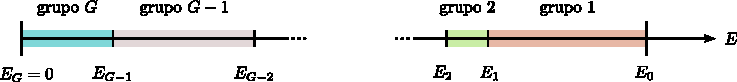
\includegraphics[width=0.95\textwidth,height=\textheight]{040-discretizacion/multigroup-energy.pdf}

}

\caption{\label{fig-multigroup}Discretización del dominio energético en
grupos (volúmenes) de energía. Tomamos la mayor energía esperada~\(E_0\)
y dividimos el intervalo~\([0,E_0]\)~en \(G\) grupos, no necesariamente
iguales. El grupo uno es el de mayor energía.}

\end{figure}

\begin{definition}[]\protect\hypertarget{def-psig}{}\label{def-psig}

El flujo angular~\(\psi_g\) del grupo~\(g\) es

\[
\psi_g(\vec{x}, \omegaversor) = \int_{E_g}^{E_{g-1}} \psi(\vec{x}, \omegaversor, E) \, dE
\]

\end{definition}

\begin{definition}[]\protect\hypertarget{def-phig}{}\label{def-phig}

El flujo escalar~\(\phi_g\) del grupo~\(g\) es

\[
\phi_g(\vec{x}) = \int_{E_g}^{E_{g-1}} \phi(\vec{x}, E) \, dE
\]

\end{definition}

\begin{definition}[]\protect\hypertarget{def-Jg}{}\label{def-Jg}

El vector corriente~\(\vec{J}_g\) del grupo~\(g\) es

\[
\vec{J}_g(\vec{x}) =
\int_{E_g}^{E_{g-1}} \vec{J}(\vec{x},E) \, dE =
\int_{E_g}^{E_{g-1}} \int_{4\pi} \psi(\vec{x}, \omegaversor, E) \cdot \omegaversor \, d\omegaversor \, dE =
\int_{4\pi} \psi_g(\vec{x}, \omegaversor) \cdot \omegaversor \, d\omegaversor =
\]

\end{definition}

\begin{remark}

Los flujos~\(\psi(\vec{x}, \omegaversor, E)\)
y~\(\psi_g(\vec{x}, \omegaversor)\) no tienen las mismas unidades. La
primera magnitud tiene unidades de inversa de área por inversa de ángulo
sólido por inversa de energía por inversa de tiempo (por
ejemplo~\(\text{cm}^{-2} \cdot \text{eV}^{-1} \cdot \text{s}^{-1}\)),
mientras que la segunda es un flujo integrado por lo que sus unidades
son inversa de área por inversa de ángulo sólido por inversa de tiempo
(por ejemplo~\(\text{cm}^{-2} \cdot \text{s}^{-1}\)). La misma idea
aplica a~\(\phi(\vec{x}, E)\) y a~\(\phi_g(\vec{x})\).

\end{remark}

Los tres objetivos de discretizar la energía en~\(G\) grupos son

\begin{enumerate}
\def\labelenumi{\arabic{enumi}.}
\tightlist
\item
  transformar la dependencia continua del flujo
  angular~\(\psi(\vec{x}, \omegaversor, E)\) con la energía~\(E\)
  en~\(G\) funciones~\(\psi_g(\vec{x},\omegaversor)\) y del flujo
  escalar~\(\phi(\vec{x}, E)\) en~\(G\) funciones~\(\phi_g(\vec{x})\),
\item
  reemplazar las integrales sobre la variable continua~\(E^\prime\) por
  sumatorias finitas sobre el índice~\(g^\prime\), y
\item
  re-escribir las ecuaciones de difusión y transporte en función de los
  flujos de grupo (\(\psi_g(\vec{x},\omegaversor)\) en transporte
  y~\(\phi_g(\vec{x})\) en difusión)
\end{enumerate}

Para ilustrar la idea, prestemos atención al término de absorción total
de la ecuación de transporte~\(\Sigma_t \cdot \psi\). El objetivo es
integrarlo con respecto a~\(E\) entre~\(E_g\) y~\(E_{g-1}\) y escribirlo
como el producto de una sección eficaz total asociada al grupo~\(g\) por
el flujo angular~\(\psi_g\) de la~definición~\ref{def-psig}:

\begin{equation}\protect\hypertarget{eq-sigmatg-psig}{}{
\int_{E_g}^{E_{g-1}} \Sigma_t(\vec{x}, E) \cdot \psi(\vec{x}, \omegaversor, E) \, dE =
\Sigma_{t g}(\vec{x}) \cdot \psi_g(\vec{x}, \omegaversor)
}\label{eq-sigmatg-psig}\end{equation}

De la misma manera, para la ecuación de difusión quisiéramos que

\[
\int_{E_g}^{E_{g-1}} \Sigma_t(\vec{x}, E) \cdot \phi(\vec{x}, E) \, dE =
\Sigma_{t g}(\vec{x}) \cdot \phi_g(\vec{x})
\]

Según la~definición~\ref{def-psig}, la sección eficaz
total~\(\Sigma_{t g}\) media en el grupo~\(g\) debe ser

\[
\Sigma_{t g}(\vec{x}) =
\frac{\displaystyle \int_{E_g}^{E_{g-1}} \Sigma_t(\vec{x}, E) \cdot \phi(\vec{x}, E) \, dE}{\displaystyle \int_{E_g}^{E_{g-1}} \phi(\vec{x}, E) \, dE}
\] con lo que no hemos ganado nada ya que llegamos a una condición
tautológica donde el parámetro que necesitamos para no tener que conocer
la dependencia explícita del flujo con la energía depende justamente de
dicha dependencia. Sin embargo ---y es ésta una de las ideas centrales
del cálculo y análisis de reactores--- podemos suponer que el cálculo de
celda (\textbf{?@sec-celda}) es capaz de proveernos las secciones eficaz
macroscópicas multigrupo para el reactor que estamos modelando de forma
tal que, desde el punto de vista del cálculo de núcleo, \(\Sigma_{t g}\)
y todas las demás secciones eficaces macroscópicas son distribuciones
conocidas del espacio~\(\vec{x}\).

Para analizar la sección eficaz de \(\nu\)-fisiones, integremos el
término de fisión de la ecuación de transporte entre las
energías~\(E_{g-1}\) y~\(E_g\) e igualémoslo a una sumatoria de
productos~\(\nu\Sigma_{fg^\prime} \cdot \phi_{g^\prime}\)\footnote{Podríamos
  haber integrado la ecuación de difusión, en cuyo caso no tendríamos el
  denominador~\(4\pi\) en ambos miembros. En cualquier caso, el
  resultado sería el mismo.}

\begin{equation}\protect\hypertarget{eq-nusigmaf-phig}{}{
\int_{E_{g-1}}^{E_g} \frac{\chi(E)}{4\pi} \cdot
\int_0^\infty \nu\Sigma_f(\vec{x},E^\prime) \cdot \phi(\vec{x}, E^\prime) \, dE^\prime \, dE
=
\frac{\chi_g}{4\pi} \cdot
\sum_{g^\prime=1}^G \nu\Sigma_{fg^\prime}(\vec{x}) \cdot \phi_{g^\prime}(\vec{x})
}\label{eq-nusigmaf-phig}\end{equation}

entonces

\begin{equation}\protect\hypertarget{eq-chig}{}{
\chi_g = \int_{E_{g-1}}^{E_g} \chi(E) \, dE
}\label{eq-chig}\end{equation} y

\[
\nu\Sigma_{f g}(\vec{x}) = \frac{\displaystyle \int_{E^\prime_g}^{E^\prime_{g-1}} \nu\Sigma_f(\vec{x}, E^\prime) \cdot \phi(\vec{x}, E^\prime) \, dE^\prime}{\displaystyle \int_{E^\prime_g}^{E^\prime_{g-1}} \phi(\vec{x}, E^\prime) \, dE^\prime}
\]

Para el término de \foreignlanguage{american}{scattering} isotrópico,
requerimos que

\begin{equation}\protect\hypertarget{eq-sigmas0-phig}{}{
\int_{E_{g-1}}^{E_g} \frac{1}{4\pi} \cdot 
\int_{0}^{\infty} \Sigma_{s_0}(\vec{x}, E^{\prime} \rightarrow E) \cdot \phi(\vec{x},E^\prime) \, dE^\prime \, dE
=
\frac{1}{4\pi} \cdot \sum_{g=1}^G \Sigma_{s_0 g^\prime \rightarrow g}(\vec{x}) \cdot \phi_{g^\prime}(\vec{x})
}\label{eq-sigmas0-phig}\end{equation} entonces

\[
\Sigma_{s_0 g^\prime \rightarrow g}(\vec{x}) =
\frac{\displaystyle \int_{E_{g-1}}^{E_g} \int_{E^\prime_{g-1}}^{E^\prime_g} \Sigma_{s_0}(\vec{x}, E^{\prime} \rightarrow E) \cdot \phi(\vec{x},E^\prime) \,dE}{\displaystyle \int_{E^\prime_{g-1}}^{E^\prime_g} \phi(\vec{x},E^\prime) \, dE^\prime}
\]

\begin{remark}

Necesitamos una doble integral sobre~\(E\) y sobre~\(E^\prime\)
porque~\(\Sigma_{s_0}(\vec{x}, E^{\prime} \rightarrow E)\) es una
sección eficaz diferencial y tiene unidades de inversa de longitud por
inversa de ángulo sólido por inversa de energía.

\end{remark}

Un análisis similar para el término de
\foreignlanguage{american}{scattering} linealmente anisotrópico

\begin{equation}\protect\hypertarget{eq-sigmas1-Jg}{}{
\int_{E_{g-1}}^{E_g} \frac{3 \cdot \omegaversor}{4\pi} \cdot 
\int_{0}^{\infty} \Sigma_{s_0}(\vec{x}, E^{\prime} \rightarrow E) \cdot \vec{J}(\vec{x},E^\prime) \, dE^\prime \, dE
=
\frac{3 \cdot \omegaversor}{4\pi} \cdot \sum_{g=1}^G \Sigma_{s_1 g^\prime \rightarrow g}(\vec{x}) \cdot \vec{J}_{g^\prime}(\vec{x})
}\label{eq-sigmas1-Jg}\end{equation} arrojaría la necesidad de pesar la
sección eficaz diferencial con la corriente~\(\vec{J}\) en lugar de con
el flujo escalar~\(\phi\), dejando una expresión sin sentido matemático
como

\[
\Sigma_{s_1 g^\prime \rightarrow g}(\vec{x}) =
\frac{\displaystyle \int_{E_{g-1}}^{E_g} \int_{E^\prime_{g-1}}^{E^\prime_g} \Sigma_{s_1}(\vec{x}, E^{\prime} \rightarrow E) \cdot \vec{J}(\vec{x},E^\prime) \,dE}{\displaystyle \int_{E^\prime_{g-1}}^{E^\prime_g} \vec{J}(\vec{x},E^\prime) \, dE^\prime}
\] a menos que tanto numerador como denominador tengan sus elementos
proporcionales entre sí y la división se tome como elemento a elemento.
Usualmente se desprecia la diferencia entre corriente y flujo y podemos
utilizar el flujo para pesar el término de
\foreignlanguage{american}{scattering} anisotrópico:

\[
\Sigma_{s_1 g^\prime \rightarrow g}(\vec{x}) \approx
\frac{\displaystyle \int_{E_{g-1}}^{E_g} \int_{E^\prime_{g-1}}^{E^\prime_g} \Sigma_{s_1}(\vec{x}, E^{\prime} \rightarrow E) \cdot \phi(\vec{x},E^\prime) \,dE}{\displaystyle \int_{E^\prime_{g-1}}^{E^\prime_g} \phi(\vec{x},E^\prime) \, dE^\prime}
\]

Integremos ahora la ecuación de
transporte~\textbf{?@eq-transporte-linealmente-anisotropica} con
respecto a~\(E\) entre~\(E_g\) y~\(E_{g-1}\):

\[
\begin{gathered}
 \omegaversor \cdot \text{grad} \left[ \int_{E_g}^{E_{g-1}} \psi(\vec{x}, \omegaversor, E) \, dE \right]  +
 \int_{E_g}^{E_{g-1}} \Sigma_t(\vec{x}, E) \cdot \psi(\vec{x}, \omegaversor, E) \, dE = \\
 \int_{E_g}^{E_{g-1}} \frac{1}{4\pi} \cdot \int_{0}^{\infty} \Sigma_{s_0}(\vec{x}, E^{\prime} \rightarrow E) \cdot \phi(\vec{x}, E^{\prime}) \, dE^\prime + \\
 \int_{E_g}^{E_{g-1}} \frac{3 \cdot \omegaversor}{4\pi} \cdot \int_{0}^{\infty} \Sigma_{s_1}(\vec{x}, E^{\prime} \rightarrow E) \cdot \vec{J}(\vec{x}, E^{\prime}) \, dE^\prime + \\
 \int_{E_g}^{E_{g-1}} \frac{\chi(E)}{4\pi} \int_{0}^{\infty} \int_{4\pi} \nu\Sigma_f(\vec{x}, E^\prime) \cdot \phi(\vec{x}, E^\prime) \, dE^\prime \, dE +
 \int_{E_g}^{E_{g-1}} s(\vec{x}, \omegaversor, E) \, dE
\end{gathered}
\]

\begin{definition}[]\protect\hypertarget{def-s-g}{}\label{def-s-g}

Definimos la fuente de neutrones independientes del grupo~\(g\) como

\[
s_g(\vec{x}, \omegaversor) = \int_{E_g}^{E_{g-1}} s(\vec{x}, \omegaversor, E) \, dE
\]

\end{definition}

\begin{definition}[]\protect\hypertarget{def-s0-g}{}\label{def-s0-g}

Definimos el momento de orden cero de las fuentes independentes del
grupo~\(g\) como

\[
s_{0g}(\vec{x}) = \int_{E_g}^{E_{g-1}} s_0(\vec{x}, E) \, dE
\]

\end{definition}

Teniendo en cuenta las definiciones

\begin{itemize}
\tightlist
\item
  \ref{def-psig}
\item
  \ref{def-phig}
\item
  \ref{def-Jg}
\item
  \ref{def-s-g}
\end{itemize}

y las ecuaciones

\begin{itemize}
\tightlist
\item
  \ref{eq-sigmatg-psig}
\item
  \ref{eq-nusigmaf-phig}
\item
  \ref{eq-chig}
\item
  \ref{eq-sigmas0-phig}
\item
  \ref{eq-sigmas1-Jg}
\end{itemize}

obtenemos las~\(G\) ecuaciones de transporte multigrupo

\begin{equation}\protect\hypertarget{eq-transportemultigrupo}{}{
\begin{gathered}
 \omegaversor \cdot \text{grad} \left[ \psi_g(\vec{x}, \omegaversor) \right]  +
 \Sigma_{t g}(\vec{x}) \cdot \psi_g(\vec{x}, \omegaversor) = 
 \frac{1}{4\pi} \cdot \sum_{g=1}^G \Sigma_{s_0 g^\prime \rightarrow g}(\vec{x}) \cdot \phi_{g^\prime}(\vec{x}) + \\
 \frac{3 \cdot \omegaversor}{4\pi} \cdot \sum_{g=1}^G \Sigma_{s_1 g^\prime \rightarrow g}(\vec{x}) \cdot \vec{J}_{g^\prime}(\vec{x}) + 
 \frac{\chi_g}{4\pi} \sum_{g^\prime=1}^G \nu\Sigma_{fg^\prime}(\vec{x}) \cdot \phi_{g^\prime}(\vec{x})
+ s_g(\vec{x}, \omegaversor)
\end{gathered}
}\label{eq-transportemultigrupo}\end{equation} donde las incógnitas
son~\(\psi_g(\vec{x}, \omegaversor)\) para~\(g=1,\dots,G\)

Procediendo de forma análoga para la ecuación de
difusión~\textbf{?@eq-difusion-ss}, primero integrándola con respecto
a~\(E\) entre~\(E_{g-1}\) y~\(E_g\) y luego teniendo en cuenta las
definiciones

\begin{itemize}
\tightlist
\item
  \ref{def-psig}
\item
  \ref{def-phig}
\item
  \ref{def-s0-g}
\end{itemize}

podemos obtener la ecuación de difusión multigrupo

\begin{equation}\protect\hypertarget{eq-difusionmultigrupo}{}{
\begin{gathered}
 - \text{div} \Big[ D_g(\vec{x}) \cdot \text{grad} \left[ \phi_g(\vec{x}) \right] \Big]
 + \Sigma_{t g}(\vec{x}) \cdot \phi_g(\vec{x})
 = \\
\sum_{g^\prime = 1}^G \Sigma_{s_0 g^\prime \rightarrow g}(\vec{x})  \cdot \phi_{g^\prime}(\vec{x}) +
\chi_g \sum_{g^\prime = 1}^G \nu\Sigma_{fg^\prime}(\vec{x}) \cdot \phi_{g^\prime}(\vec{x})+ s_{0g}(\vec{x})
\end{gathered}
}\label{eq-difusionmultigrupo}\end{equation} donde ahora las incógnitas
son~\(\phi_g(\vec{x})\) para~\(g=1,\dots,G\),

\begin{remark}

El coeficiente de difusión~\(D_g\) del grupo~\(g\) proviene de calcular
las secciones eficaces~\(\Sigma_{tg}\), \(\Sigma_{st}\) y el coseno
medio de \foreignlanguage{american}{scattering}~\(\mu_{0g}\) del
grupo~\(g\) y reemplazar la~\textbf{?@def-D} por

\begin{equation}\protect\hypertarget{eq-D}{}{
D_g(\vec{x}) = \frac{1}{3 \left[ \Sigma_{tg}(\vec{x}) - \mu_{0g}(\vec{x}) \cdot \Sigma_{s_t g}(\vec{x}) \right]}
}\label{eq-D}\end{equation}

\end{remark}

\begin{remark}

Matemáticamente, la aproximación multigrupo es equivalente a discretizar
el dominio de la energía con un esquema de volúmenes finitos con la
salvedad de que no hay operadores diferenciales con respecto a la
variable~\(E\) sino que el acople entre volúmenes se realiza en forma
algebraica. Dicho acople no es necesariamente entre primeros vecinos
solamente sino que es arbitrario, i.e.~un neutrón puede pasar del grupo
1 al~\(G\), o viceversa, o de un grupo arbitrario~\(g^\prime\) a otro
grupo~\(g\).

\end{remark}

\begin{remark}

Dado que en las ecuaciones multigrupo~\ref{eq-transportemultigrupo} y
\ref{eq-difusionmultigrupo} la discretización es estrictamente
algebraica y deliberadamente tautológica, la consistencia es
teóricamente fuerte ya que el operador discretizado coincide con el
operador continuo incluso para un único grupo de energías~\(G=1\). De
hecho las ecuaciones multigrupo se basan solamente en
\emph{definiciones}. En la práctica, la consistencia depende del cálculo
a nivel de celda de la~\textbf{?@sec-celda}.

\end{remark}

\hypertarget{sec-sn}{%
\section{Discretización en ángulo}\label{sec-sn}}

Para discretizar la dependencia espacial de la ecuación de transporte
multigrupo~\ref{eq-transportemultigrupo} aplicamos el método de
ordenadas discretas o~S\(_N\), discutido en la literatura tradicional de
física de reactores. En esta tesis lo derivamos al integrar las
ecuaciones multigrupo continuas en~\(\omegaversor\) sobre volúmenes de
control finitos como si fuese un esquema numérico basado en el método de
volúmenes finitos. De hecho, en este caso, los volúmenes finitos son
áreas~\(\Delta \omegaversor_m\) discretas de la esfera unitaria donde
cada una de ellas tiene asociadas

\begin{enumerate}
\def\labelenumi{\arabic{enumi}.}
\tightlist
\item
  un peso~\(w_m\)
\item
  una dirección particular~\(\omegaversor_m\), y
\item
  una fracción de total de área unitaria~\(\Delta \omegaversor_m/4\pi\)
\end{enumerate}

para~\(m=1,\dots,M\). Nuevamente el acople entre volúmenes de control es
algebraico y no necesariamente a primeros vecinos.

\begin{theorem}[de cuadratura sobre la esfera
unitaria]\protect\hypertarget{thm-cuadratura}{}\label{thm-cuadratura}

La integral de una función escalar~\(f(\omegaversor)\) de cuadrado
integrable sobre todas las direcciones~\(\omegaversor\) es igual
a~\(4\pi\) veces la suma de un conjunto de~\(M\) pesos~\(w_m\)
normalizados tal que \(\sum w_m = 1\), mutiplicados por~\(M\) valores
medios~\(\left\langle f(\omegaversor)\right\rangle_m\) asociados a~\(M\)
direcciones~\(\omegaversor_m\) donde cada una de las cuales tiene
asociada también una porción~\(\Delta \omegaversor_m\) de la esfera
unitaria tal que su unión es~\(4\pi\) y su intersección es cero:

\[
\int_{4\pi} f(\omegaversor) \, d\omegaversor = 4\pi \cdot \sum_{w=1}^M w_m \cdot \left\langle f(\omegaversor)\right\rangle_m
\]

El peso~\(w_m\) es

\[
w_m = \frac{1}{4\pi} \cdot \int_{\Delta \omegaversor_m} d\omegaversor =
\frac{\Delta \omegaversor_m}{4\pi}
\]

\begin{proof}

Comenzamos escribiendo la integral sobre~\(4\pi\) como una suma
para~\(m=1,\dots,M\)

\[
 \int_{4\pi} f(\omegaversor) \, d\omegaversor = \sum_{m=1}^M \int_{\Delta \omegaversor_m} f(\omegaversor) \, d\omegaversor
\]

Multiplicamos y dividimos por
\(\int_{\Delta \omegaversor_m} d\omegaversor = 4\pi \cdot w_m\)

\[
\sum_{m=1}^M \int_{\Delta \omegaversor_m} f(\omegaversor) \, d\omegaversor
= \sum_{m=1}^M \frac{ \displaystyle \int_{\Delta \omegaversor_m} f(\omegaversor) \, d\omegaversor}{ \displaystyle \int_{\Delta \omegaversor_m} d\omegaversor} \cdot \int_{\Delta \omegaversor_m} d\omegaversor
= \sum_{m=1}^M \frac{ \displaystyle \int_{\Delta \omegaversor_m} f(\omegaversor) \, d\omegaversor}{ \displaystyle \int_{\Delta \omegaversor_m} d\omegaversor} \cdot 4\pi \, w_m
\]

Si
llamamos~\(\left\langle f(\omegaversor)\right\rangle_{\omegaversor_m}\)
al valor medio de~\(f\) en~\(\Delta \omegaversor_m\)

\[
\left\langle f(\omegaversor)\right\rangle_{\omegaversor_m} = \frac{ \displaystyle \int_{\Delta \omegaversor_m} f(\omegaversor) \, d\omegaversor}{ \displaystyle \int_{\Delta \omegaversor_m} d\omegaversor}
\] entonces se sigue la tesis del teorema.

\end{proof}

\end{theorem}

\begin{definition}[]\protect\hypertarget{def-psi-mg}{}\label{def-psi-mg}

El flujo angular~\(\psi_{mg}\) del grupo~\(g\) asociado a la ordenada
discreta~\(m\) es igual al valor medio del flujo angular~\(\psi_g\) del
grupo~\(g\) (definido en la~definición~\ref{def-psig}) alrededor de la
dirección~\(\omegaversor_m\):

\[
\psi_{mg}(\vec{x}) = \left\langle \psi_g(\vec{x},\omegaversor)\right\rangle_{\omegaversor_m} = \frac{ \displaystyle \int_{\Delta \omegaversor_m} \psi_g(\vec{x},\omegaversor) \, d\omegaversor}{ \displaystyle \int_{\Delta \omegaversor_m} d\omegaversor}
\]

\end{definition}

\begin{remark}

Esta vez~\(\psi_{mg}\) sí tiene la mismas unidades que~\(\psi_{g}\).

\end{remark}

\begin{corollary}[]\protect\hypertarget{cor-int-psi-g}{}\label{cor-int-psi-g}

La integral del flujo escalar sobre la porción~\(\Delta \omegaversor_m\)
de la esfera unitaria es~\(4\pi\) veces el
producto~\(w_m \cdot \psi_{mg}\):

\[
\int_{\Delta \omegaversor_m} \psi_g(\vec{x},\omegaversor) \, d\omegaversor
=
\psi_{mg}(\vec{x}) \cdot \Delta \omegaversor_m 
=
4\pi \cdot w_m \cdot \psi_{mg}(\vec{x})
\]

\end{corollary}

\begin{corollary}[]\protect\hypertarget{cor-phig-sum-psimg}{}\label{cor-phig-sum-psimg}

El flujo escalar~\(\phi_g\) del grupo~\(g\) es igual a

\[
\phi_g(\vec{x}) = \int_{4\pi} \psi_g(\vec{x}, \omegaversor) \, d\omegaversor =
4\pi \sum_{m=1}^M w_m \cdot \psi_{mg}(\vec{x})
\]

\end{corollary}

Re-escribamos primero la~ecuación~\ref{eq-transportemultigrupo} de
transporte multigrupo \[\tag{\ref{eq-transportemultigrupo}}
\begin{gathered}
 \omegaversor \cdot \text{grad} \left[ \psi_g(\vec{x}, \omegaversor) \right]  +
 \Sigma_{t g}(\vec{x}) \cdot \psi_g(\vec{x}, \omegaversor) = 
 \frac{1}{4\pi} \cdot \sum_{g=1}^G \Sigma_{s_0 g^\prime \rightarrow g}(\vec{x}) \cdot \phi_{g^\prime}(\vec{x}) + \\
 \frac{3 \cdot \omegaversor}{4\pi} \cdot \sum_{g=1}^G \Sigma_{s_1 g^\prime \rightarrow g}(\vec{x}) \cdot \vec{J}_{g^\prime}(\vec{x}) + 
 \frac{\chi_g}{4\pi} \sum_{g^\prime=1}^G \nu\Sigma_{fg^\prime}(\vec{x}) \cdot \phi_{g^\prime}(\vec{x})
+ s_g(\vec{x}, \omegaversor)
\end{gathered}
\]

en función de los flujos angulares~\(\psi_{mg}\) usando
la~definición~\ref{def-psi-mg} y explicitando el termino de la corriente
como la integral del producto \(\psi_{g^\prime} \cdot \omegaversor\)
según la~definición~\ref{def-Jg}

\[
\begin{gathered}
 \omegaversor \cdot \text{grad} \left[ \psi_g(\vec{x}, \omegaversor) \right]  +
 \Sigma_{t g}(\vec{x}) \cdot \psi_g(\vec{x}, \omegaversor) = \\
 \frac{1}{4\pi} \cdot \sum_{g=1}^G \Sigma_{s_0 g^\prime \rightarrow g}(\vec{x}) \cdot 4\pi \cdot \sum_{m^\prime=1} w_{m^\prime} \cdot \psi_{m^\prime g^\prime}(\vec{x}) + \\
 \frac{3 \cdot \omegaversor}{4\pi} \cdot \sum_{g=1}^G \Sigma_{s_1 g^\prime \rightarrow g}(\vec{x}) \cdot \sum_{m^\prime=1} \int_{\omegaversor_{m^\prime}} \psi_{g^\prime}(\vec{x},\omegaversor) \cdot \omegaversor \, d\omegaversor +\\
 \frac{\chi_g}{4\pi} \sum_{g^\prime=1}^G \nu\Sigma_{fg^\prime}(\vec{x})\cdot 4\pi \cdot \sum_{m^\prime=1} w_{m^\prime} \cdot \psi_{m^\prime g^\prime}(\vec{x})
+ s_g(\vec{x}, \omegaversor)
\end{gathered}
\]

Ahora cancelamos los factores~\(4\pi\) en los términos de
\foreignlanguage{american}{scattering} lineal y fisión, integramos todos
los términos con respecto a~\(\omegaversor\)
sobre~\(\Delta \omegaversor_m\) y los analizamos uno por uno:

\begin{equation}\protect\hypertarget{eq-trasporte-integrado-omegam}{}{
\begin{gathered}
 \underbrace{\int_{\omegaversor_m} \left\{ \omegaversor \cdot \text{grad} \left[ \psi_g(\vec{x}, \omegaversor) \right] \right\} \, d\omegaversor}_\text{advección} +
 \underbrace{\int_{\omegaversor_m} \left\{ \Sigma_{t g}(\vec{x}) \cdot \psi_g(\vec{x}, \omegaversor)  \right\} \, d\omegaversor}_\text{absorción total} = \\
 \underbrace{\bigintsss_{\omegaversor_m} \left\{ \sum_{g=1}^G \Sigma_{s_0 g^\prime \rightarrow g}(\vec{x})  \cdot \sum_{m^\prime=1} w_{m^\prime} \cdot \psi_{m^\prime g^\prime}(\vec{x}) \right\}  \, d\omegaversor}_\text{scattering isotrópico} + \\
 \underbrace{\bigintsss_{\omegaversor_m} \left\{ \frac{3 \cdot \omegaversor}{4\pi} \cdot \sum_{g=1}^G \Sigma_{s_1 g^\prime \rightarrow g}(\vec{x}) \cdot \sum_{m^\prime=1} \int_{\omegaversor_{m^\prime}} \psi_{g^\prime}(\vec{x},\omegaversor^\prime) \cdot \omegaversor^\prime \, d\omegaversor^\prime   \right\} \, d\omegaversor}_\text{scattering linealmente anisotrópico} +\\
 \underbrace{\bigintsss_{\omegaversor_m} \left\{ \chi_g \cdot \sum_{g^\prime=1}^G \nu\Sigma_{fg^\prime}(\vec{x}) \cdot   \sum_{m^\prime=1} w_{m^\prime} \cdot \psi_{m^\prime g^\prime}(\vec{x}) \right\}  \, d\omegaversor}_\text{fisión} +
 \underbrace{\int_{\omegaversor_m} \left\{ s_g(\vec{x}, \omegaversor)  \right\} \, d\omegaversor  }_\text{fuentes independientes}
\end{gathered}
}\label{eq-trasporte-integrado-omegam}\end{equation}

Comencemos por el termino de advección, revirtiendo
el~\textbf{?@thm-div-inner}

\[
\begin{aligned}
\int_{\omegaversor_m} \left\{ \omegaversor \cdot \text{grad} \left[ \psi_g(\vec{x}, \omegaversor) \right] \right\} \, d\omegaversor
&=
\int_{\omegaversor_m}  \text{div} \left[ \omegaversor \cdot \psi_g(\vec{x}, \omegaversor) \right] \, d\omegaversor
\\
&=
\text{div} \left[ \int_{\omegaversor_m} \omegaversor \cdot \psi_g(\vec{x}, \omegaversor) \, d\omegaversor \right]
\end{aligned}
\]

Prestemos atención a la integral. Supongamos que el flujo angular es
constante a trozos\footnote{Del ingles
  \foreignlanguage{american}{\emph{piecewise constant}}.} dentro de cada
área~\(\Delta \omegaversor_m\). Entonces este valor constante es igual
al valor medio de~\(\psi\) en~\(\Delta \omegaversor_m\)

\[
\psi_g(\vec{x}, \omegaversor) = \left\langle \psi_g(\vec{x}, \omegaversor) \right\rangle_{\omegaversor_m} = \psi_{mg}(\vec{x})
\quad \text{si $\omegaversor \in \Delta \omegaversor_m$}
\]

En estas condiciones, \(\psi\) puede salir de la integral

\[
\int_{\omegaversor_m} \omegaversor \cdot \psi_g(\vec{x}, \omegaversor) \, d\omegaversor
\approx
\psi_{mg}(\vec{x}) \cdot \int_{\omegaversor_m} \omegaversor \, d\omegaversor
\]

\begin{definition}[]\protect\hypertarget{def-mean-omega}{}\label{def-mean-omega}

Llamamos~\(\omegaversor_m\) a la direccion que resulta ser el valor
medio~\(\left\langle \omegaversor \right\rangle_{\omegaversor_m}\) de
todas las direcciones integradas en el area~\(\Delta \omegaversor_m\)
sobre la esfera unitaria, es decir

\[
\omegaversor_m = \left\langle \omegaversor \right\rangle_{\omegaversor_m} =
\frac{ \displaystyle \int_{\Delta \omegaversor_m} \omegaversor \, d\omegaversor}{ \displaystyle \int_{\Delta \omegaversor_m} d\omegaversor}
\]

\end{definition}

\begin{corollary}[]\protect\hypertarget{cor-int-omega}{}\label{cor-int-omega}

La integral del versor~\(\omegaversor\) sobre la
fracción~\(\Delta \omegaversor_m\) de la esfera unitaria es igual al
producto de~\(\omegaversor_m\) por~\(\Delta \omegaversor_m\):

\[
\int_{\Delta \omegaversor_m} \omegaversor \, d\omegaversor
=
\omegaversor_m \cdot \Delta \omegaversor_m 
\]

\end{corollary}

\begin{corollary}[]\protect\hypertarget{cor-int-psig-omega}{}\label{cor-int-psig-omega}

La integral del producto del versor~\(\omegaversor\) con el flujo
angular del grupo~\(g\) sobre~\(\Delta \omegaversor_m\) es
aproximadamente igual al
producto~\(\psi_{mg} \cdot \Delta \omegaversor_m\):

\[
\int_{\omegaversor_m} \omegaversor \cdot \psi_g(\vec{x}, \omegaversor) \, d\omegaversor
\approx
\omegaversor_m \cdot \psi_{mg}(\vec{x}) \cdot  \Delta \omegaversor_m 
\]

\end{corollary}

Podemos volver a aplicar el~\textbf{?@thm-div-inner} para escribir el
término de advección como

\begin{equation}\protect\hypertarget{eq-sn-adveccion}{}{
\begin{aligned}
\text{div} \left[ \int_{\omegaversor_m} \omegaversor \cdot \psi_g(\vec{x}, \omegaversor) \, d\omegaversor \right]
& \approx
\text{div} \left[ \omegaversor_m \cdot \psi_{mg}(\vec{x}) \cdot  \Delta \omegaversor_m  \right] \\
& \approx
\omegaversor_m \cdot \text{grad} \left[ \psi_{mg}(\vec{x}) \right]  \cdot \Delta \omegaversor_m \\
\end{aligned}
}\label{eq-sn-adveccion}\end{equation}

Pasemos ahora al término de absorciones totales de
la~ecuación~\ref{eq-trasporte-integrado-omegam}. La sección eficaz no
depende de~\(\omegaversor\) por lo que puede salir fuera de la integral

\[
\int_{\omegaversor_m} \left\{ \Sigma_{t g}(\vec{x}) \cdot \psi_g(\vec{x}, \omegaversor)  \right\} \, d\omegaversor = \Sigma_{t g}(\vec{x}) \cdot
\int_{\omegaversor_m} \psi_g(\vec{x}, \omegaversor) \, d\omegaversor
\]

Por el~corolario~\ref{cor-int-psi-g} la última integral
es~\(\psi_{mg} \cdot \Delta \omegaversor_m\), entonces

\begin{equation}\protect\hypertarget{eq-sn-absorciones}{}{
\int_{\omegaversor_m} \left[ \Sigma_{t g}(\vec{x}) \cdot \psi_g(\vec{x}, \omegaversor)  \right] \, d\omegaversor = \left[ \Sigma_{t g}(\vec{x}) \cdot \psi_{mg}(\vec{x}) \right] \cdot \Delta \omegaversor_m
}\label{eq-sn-absorciones}\end{equation}

El término de \foreignlanguage{american}{scattering} isotrópico queda

\begin{equation}\protect\hypertarget{eq-sn-scattering-isotropico}{}{
\bigintsss_{\omegaversor_m} \sum_{g=1}^G \Sigma_{s_0 g^\prime \rightarrow g}(\vec{x})  \cdot \sum_{m^\prime=1} w_{m^\prime} \cdot \psi_{m^\prime g^\prime}(\vec{x}) \, d\omegaversor
=
\left[ \sum_{g=1}^G \Sigma_{s_0 g^\prime \rightarrow g}(\vec{x})  \cdot \sum_{m^\prime=1} w_{m^\prime} \cdot \psi_{m^\prime g^\prime}(\vec{x}) \right] \cdot \Delta \omegaversor_m
}\label{eq-sn-scattering-isotropico}\end{equation} ya que el integrando
no depende de~\(\omegaversor\).

El integrando del término de \foreignlanguage{american}{scattering}
linealmente anisotrópico sí depende de~\(\omegaversor\).

\[
\bigintsss_{\omegaversor_m} \left[ \frac{3 \cdot \omegaversor}{4\pi} \cdot \sum_{g=1}^G \Sigma_{s_1 g^\prime \rightarrow g}(\vec{x}) \cdot \sum_{m^\prime=1} \int_{\omegaversor_{m^\prime}} \psi_{g^\prime}(\vec{x},\omegaversor^\prime) \cdot \omegaversor^\prime \, d\omegaversor^\prime   \right] \, d\omegaversor
\]

Primero notamos que el corolario~\ref{cor-int-psig-omega} nos indica, de
manera aproximada, el resultado de la integral
sobre~\(\omegaversor_{m^\prime}\):
\(\omegaversor_{m^\prime} \psi_{m^\prime g^\prime} \Delta\omegaversor_{m^\prime}\).
A su vez, \(\Delta\omegaversor_{m^\prime} = 4\pi w_{m^\prime}\), por lo
que

\[
\begin{gathered}
\bigintsss_{\omegaversor_m} \left[ \frac{3 \cdot \omegaversor}{4\pi} \cdot \sum_{g=1}^G \Sigma_{s_1 g^\prime \rightarrow g}(\vec{x}) \cdot \sum_{m^\prime=1} 4\pi \cdot w_{m^\prime} \cdot \psi_{m^\prime g^\prime}(\vec{x}) \cdot \omegaversor_{m^\prime} \right] \, d\omegaversor
= \\
3 \sum_{g=1}^G \Sigma_{s_1 g^\prime \rightarrow g}(\vec{x}) \cdot \sum_{m^\prime=1} w_{m^\prime} \cdot \psi_{m^\prime g^\prime}(\vec{x}) \cdot \omegaversor_{m^\prime} \int_{\omegaversor_m} \omegaversor \, d\omegaversor
\end{gathered}
\]

Una vez mas, la integral sobre~\(\omegaversor_m\) ya la hemos resuelto
(exactamente) en el~corolario~\ref{cor-int-omega}, y es igual
a~\(\omegaversor_m \cdot \Delta \omegaversor_m\). Entonces el término de
\foreignlanguage{american}{scattering} linealmente anisotrópico es
aproximadamente igual a
\begin{equation}\protect\hypertarget{eq-sn-scattering-anisotropico}{}{
\begin{gathered}
\bigintsss_{\omegaversor_m} \left[ \frac{3 \cdot \omegaversor}{4\pi} \cdot \sum_{g=1}^G \Sigma_{s_1 g^\prime \rightarrow g}(\vec{x}) \cdot \sum_{m^\prime=1} \int_{\omegaversor_{m^\prime}} \psi_{g^\prime}(\vec{x},\omegaversor^\prime) \cdot \omegaversor^\prime \, d\omegaversor^\prime   \right] \, d\omegaversor
\approx \\
\left[ 3 \cdot \sum_{g=1}^G \Sigma_{s_1 g^\prime \rightarrow g}(\vec{x}) \cdot \sum_{m^\prime=1} w_{m^\prime} \cdot \left( \omegaversor_{m} \cdot \omegaversor_{m^\prime} \right) \cdot \psi_{m^\prime g^\prime}(\vec{x}) \right] \cdot  \Delta \omegaversor_m
\end{gathered}
}\label{eq-sn-scattering-anisotropico}\end{equation}

El término de fisiones es similar al de
\foreignlanguage{american}{scattering} isotrópico en el sentido de que
el integrando no depende de~\(\omegaversor\) entonces su integral
sobre~\(\Delta \omegaversor_m\) es directamente

\begin{equation}\protect\hypertarget{eq-sn-fisiones}{}{
\bigintsss_{\omegaversor_m} \chi_g \sum_{g^\prime=1}^G \nu\Sigma_{fg^\prime}(\vec{x}) \cdot   \sum_{m^\prime=1} w_{m^\prime} \cdot \psi_{m^\prime g^\prime}(\vec{x}) \, d\omegaversor
=
\left[ \chi_g \sum_{g^\prime=1}^G \nu\Sigma_{fg^\prime}(\vec{x}) \cdot   \sum_{m^\prime=1} w_{m^\prime} \cdot \psi_{m^\prime g^\prime}(\vec{x}) \right] \cdot \Delta \omegaversor_m
}\label{eq-sn-fisiones}\end{equation}

Para completar el análisis de
la~ecuación~\ref{eq-trasporte-integrado-omegam}, en el término de las
fuentes independientes usamos el concepto de valor medio

\[
\int_{\omegaversor_m} s_g(\vec{x}, \omegaversor) \, d\omegaversor
=
\left\langle s_g(\vec{x}, \omegaversor)  \right\rangle_{\omegaversor_m} \cdot \Delta \omegaversor
\]

\begin{definition}[]\protect\hypertarget{def-s-mg}{}\label{def-s-mg}

En forma análoga a la~definición~\ref{def-psi-mg}, definimos a la fuente
independiente del grupo~\(g\) en la dirección~\(m\) como

\[
s_{mg}(\vec{x}) = \left\langle s(\vec{x},\omegaversor)\right\rangle_{\omegaversor_m} = \frac{ \displaystyle \int_{\Delta \omegaversor_m} s_g(\vec{x},\omegaversor) \, d\omegaversor}{ \displaystyle \int_{\Delta \omegaversor_m} d\omegaversor}
\]

\end{definition}

El término de fuentes independientes es entonces

\begin{equation}\protect\hypertarget{eq-sn-fuentes}{}{
\int_{\omegaversor_m} s_g(\vec{x}, \omegaversor) \, d\omegaversor
=
s_{mg}(\vec{x}) \cdot \Delta \omegaversor_m
}\label{eq-sn-fuentes}\end{equation}

Juntemos ahora las ecuaciones

\begin{itemize}
\tightlist
\item
  \ref{eq-sn-adveccion} (advección)
\item
  \ref{eq-sn-absorciones} (absorciones)
\item
  \ref{eq-sn-scattering-isotropico}
  (\foreignlanguage{american}{scattering} isotrópico)
\item
  \ref{eq-sn-scattering-anisotropico}
  (\foreignlanguage{american}{scattering} linealmente anisotrópico)
\item
  \ref{eq-sn-fisiones} (fisiones)
\item
  \ref{eq-sn-fuentes} (fuentes independentes)
\end{itemize}

para re-escribir la~ecuación~\ref{eq-trasporte-integrado-omegam} como

\[
\begin{gathered}
\left[ \omegaversor_m \cdot \text{grad} \left[ \psi_{mg}(\vec{x}) \right] \right]  \cdot \Delta \omegaversor_m +
\left[ \Sigma_{t g}(\vec{x}) \cdot \psi_{mg}(\vec{x}) \right] \cdot \Delta \omegaversor_m = \\
\left[ \sum_{g=1}^G \Sigma_{s_0 g^\prime \rightarrow g}(\vec{x})  \cdot \sum_{m^\prime=1} w_{m^\prime} \cdot \psi_{m^\prime g^\prime}(\vec{x}) \right] \cdot \Delta \omegaversor_m + \\
\left[ 3 \sum_{g=1}^G \Sigma_{s_1 g^\prime \rightarrow g}(\vec{x}) \cdot \sum_{m^\prime=1} w_{m^\prime} \cdot \left( \omegaversor_{m} \cdot \omegaversor_{m^\prime} \right) \cdot \psi_{m^\prime g^\prime}(\vec{x}) \right] \cdot  \Delta \omegaversor_m + \\
\left[ \chi_g \sum_{g^\prime=1}^G \nu\Sigma_{fg^\prime}(\vec{x}) \cdot   \sum_{m^\prime=1} w_{m^\prime} \cdot \psi_{m^\prime g^\prime}(\vec{x}) \right] \cdot \Delta \omegaversor_m + 
s_{mg}(\vec{x}) \cdot \Delta \omegaversor_m
\end{gathered}
\]

Dividiendo ambos miembros por~\(\Delta \omegaversor\) obtenemos las
\(MG\) ecuaciones diferenciales de transporte en~\(G\) grupos de
energías y~\(M\) direcciones angulares, según la discretización angular
denominada en la literatura ``ordenadas discretas''

\begin{equation}\protect\hypertarget{eq-transporte-sn}{}{
\begin{gathered}
 \omegaversor_m \cdot \text{grad} \left[ \psi_{mg}(\vec{x}) \right]  +
 \Sigma_{t g}(\vec{x}) \cdot \psi_{mg}(\vec{x}) = 
 \sum_{g=1}^G \Sigma_{s_0 g^\prime \rightarrow g}(\vec{x})  \sum_{m^\prime=1} w_{m^\prime} \psi_{m^\prime g^\prime}(\vec{x})  + \\
 3  \sum_{g=1}^G \Sigma_{s_1 g^\prime \rightarrow g}(\vec{x}) \sum_{m^\prime=1} w_{m^\prime} \left( \omegaversor_{m} \cdot \omegaversor_{m^\prime} \right) \psi_{m^\prime g^\prime}(\vec{x}) + 
 \chi_g \sum_{g^\prime=1}^G \nu\Sigma_{fg^\prime}(\vec{x})   \sum_{m^\prime=1} w_{m^\prime} \psi_{m^\prime g^\prime}(\vec{x}) + 
s_{mg}(\vec{x})
\end{gathered}
}\label{eq-transporte-sn}\end{equation}

\begin{remark}

El único operador diferencial que aparece en
la~ecuación~\ref{eq-transporte-sn} es el gradiente espacial del flujo
angular~\(\psi_{mg}\) del grupo~\(g\) en la dirección~\(m\) en el
término de advección.

\end{remark}

\begin{remark}

Todos los operadores integrales que estaban presentes en
la~\textbf{?@eq-transporte-linealmente-anisotropica} han sido
reemplazados por sumatorias finitas.

\end{remark}

\begin{remark}

La única aproximación numérica que tuvimos que hacer para obtener
la~ecuación~\ref{eq-transporte-sn} a partir de la
ecuación~\ref{eq-transportemultigrupo} fue suponer que el flujo
angular~\(\psi_g\) es uniforme a trozos en cada segmento de
área~\(\Delta \omegaversor_m\) en los términos de

\begin{enumerate}
\def\labelenumi{\alph{enumi}.}
\tightlist
\item
  absorciones totales (ecuación~\ref{eq-sn-absorciones}), y
\item
  scattering linealmente anisotrópico
  (ecuación~\ref{eq-sn-scattering-anisotropico}).
\end{enumerate}

Por ejemplo, la~figura~\ref{fig-constant-per-fraction} ilustra un caso
en el que cada octante de la esfera unitaria está dividido en tres áreas
iguales, dando lugar a \(M = 3 \times 8 = 24\) direcciones. En cada una
de las áreas mostradas, asumimos que el flujo
angular~\(\psi(\vec{x},\omegaversor)\) es uniformemente igual
a~\(\psi_{mg}(\vec{x})\), siendo~\(\vec{x}\) en este caso la posición
del centro de la esfera unidad. Esta suposición es usual en los esquemas
basados en el método de volúmenes finitos.

\end{remark}

\begin{figure}

{\centering 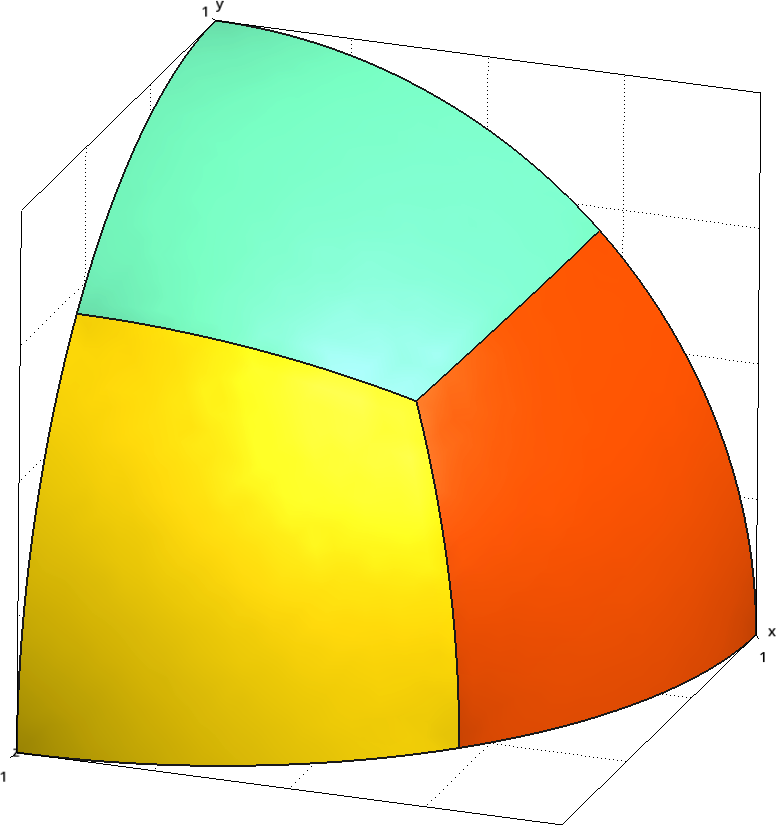
\includegraphics[width=0.5\textwidth,height=\textheight]{040-discretizacion/constant-per-fraction.png}

}

\caption{\label{fig-constant-per-fraction}Una partición de la esfera
unidad en 24 fracciones de área, todas iguales entre sí. La suposición
central de la derivación del método~\(S_N\) realizado en esta tesis es
que en cada una de éstas áreas el flujo angular es constante. Se muestra
sólo el primero de los ocho octantes.}

\end{figure}

\begin{remark}

El esquema numérico es consistente ya que en el
límite~\(\Delta \omegaversor_m \rightarrow d\omegaversor_m\) la
suposición es exacta y el operador discretizado coincide con el operador
continuo.

\end{remark}

\hypertarget{sec-cuadraturas}{%
\subsection{Conjuntos de cuadraturas en tres
dimensiones}\label{sec-cuadraturas}}

Para completar el método de las ordenadas discretas debemos
especificar~\(M\) pares de direcciones y
pesos~\((\boldsymbol{\hat\Omega}_m, w_m)\) para~\(m=1,\dots,M\). Las
direcciones~\(\boldsymbol{\hat\Omega}_m = [\hat{\Omega}_{mx} \, \hat{\Omega}_{my} \, \hat{\Omega}_{mz}]^T\)
deben ser versores unitarios tales que

\[\label{eq:normalizaciondirecciones}
 \hat{\Omega}_{mx}^2 + \hat{\Omega}_{my}^2 + \hat{\Omega}_{mz}^2 = 1\] y
los pesos~\(w_m\) deben estar normalizados a uno, es decir

\[\label{eq:normalizacionpesos}
 \sum_{m=1}^M w_m = 1\]

Existen varias maneras de elegir los~\(M\) pares de forma tal de cumplir
estas dos condiciones. En este trabajo utilizamos la cuadratura de nivel
simétrico~{[}5{]} o de simetría completa~{[}6{]} en la que las
direcciones son simétricas por octante. En un espacio de tres
dimensiones, el orden~\(N\) de la aproximación~S\(_N\) se relaciona con
la cantidad de direcciones~\(M\) como

\[M = N\cdot(N+2)\]

En este caso, en cada octante tomamos los cosenos
directores~\(\hat{\Omega}_{mx}\), \(\hat{\Omega}_{my}\)
y~\(\hat{\Omega}_{mz}\) de un conjunto de~\(N/2\) valores positivos y
los permutamos de todas las maneras posibles para obtener~\(N(N+2)/8\)
combinaciones en el primer octante para luego reflejar estas direcciones
hasta completar los ocho octantes. De esta forma las~\(M\) direcciones
son simétricas con respecto a rotaciones de noventa y ciento ochenta
grados sobre cualesquiera de los ejes~\(x\), \(y\) ó \(z\).

Debido a estas restricciones de simetría, no todos los~\(N/2\) posibles
cosenos directores son independientes. De hecho, en el caso general sólo
podemos elegir un único valor. En efecto,
sean~\(\mu_1 < \mu_2 < \dots < \mu_{N/2}\) los posibles cosenos
directores del conjunto. Supongamos que~\(\hat{\Omega}_{mx} = \mu_i\),
\(\hat{\Omega}_{my} = \mu_j\) y~\(\hat{\Omega}_{mz} = \mu_k\). Entonces

\[\label{eq:omega1}
 \mu_i^2 + \mu_j^2 + \mu_k^2 = 1\]

Tomemos ahora otra dirección diferente~\(m^\prime\) pero manteniendo el
primer componente~\(\hat{\Omega}_{m^\prime x} = \mu_i\) y
haciendo~\(\hat{\Omega}_{m^\prime y} = \mu_{j+1}\). Para poder
satisfacer la condición de magnitud unitaria y debido a
que~\(\mu_{j+1}>\mu{j}\)
entonces~\(\hat{\Omega}_{m^\prime z} = \mu_{k-1}\) ya
que~\(\mu_{k-1}<\mu_k\). Entonces

\[\label{eq:omega2}
 \mu_i^2 + \mu_{j+1}^2 + \mu_{k-1}^2 = 1\]

De~\protect\hyperlink{eq:omega1}{{[}eq:omega1{]}}
y~\protect\hyperlink{eq:omega2}{{[}eq:omega2{]}} obtenemos

\[\mu_{j+1}^2 - \mu_{j} = \mu_{k}^2 - \mu_{k-1}^2\]

Como esta ecuación debe cumplirse para todo~\(j\) y para todo~\(k\),
entonces debe ser

\[\mu_i^2 = \mu_{i-1} + C\] para todo~\(1 < i \leq N/2\), con~\(C\) una
constante a determinar. Luego

\[\mu_i^2 = \mu_{1} + C(i-1)\]

Si tomamos~\(\hat{\Omega}_{mx} = \hat{\Omega}_{my} = \mu_1\)
y~\(\hat{\Omega}_{mz}=\mu_{N/2}\), por la condición de magnitud unitaria
debe ser \(2\mu_1^2 + \mu_{N/2}^2 = 1\) por lo que podemos determinar la
constante~\(C\) como

\[C = \frac{2 (1 - 3\mu_1^2)}{N-2}\]

Finalmente, una vez seleccionado el coseno director~\(\mu_1\), podemos
calcular el resto de los~\(N/2-1\) valores como

\[\label{eq:cosenos}
 \mu_{i} = \sqrt{\mu_1^2 + (2 - 6\mu_1^2) \cdot \frac{(i-1)}{N-2}}\]
para~\(i=2,\dots,N/2\).

Las condiciones de simetría requieren que los pesos~\(w_m\)
y~\(w_{m^\prime}\) asociados a dos
direcciones~\(\boldsymbol{\hat\Omega}_m\)
y~\(\boldsymbol{\hat\Omega}_{m^\prime}\) cuyos cosenos directores son
permutaciones entre sí deben ser iguales. Además es deseable que los
pesos~\(w_m\) sean tales que la cuadratura ilustrada en la
ecuación~\protect\hyperlink{eq:cuadratura}{{[}eq:cuadratura{]}} sea lo
más aproximada posible. El cálculo detallado de los pesos está fuera del
alcance de este trabajo y nos limitamos a reportar los valores
utilizados por el código computacional desarrollado para esta tesis y
descripto en el
capítulo~\protect\hyperlink{cap:implementacion}{{[}cap:implementacion{]}}.

\begin{table}

\begin{minipage}[t]{\linewidth}

{\centering 

\begin{tabular}[t]{llclclc}
\toprule
 &  & \(\mu_1\) &  & \(m\) &  & \(8 \cdot w_i\)\\
\midrule
S\(_4\) &  & 0.3500212 &  & 1 &  & 1/3\\
S\(_6\) &  & 0.2666355 &  & 1 &  & 0.1761263\\
 &  &  &  & 2 &  & 0.1572071\\
S\(_8\) &  & 0.2182179 &  & 1 &  & 0.1209877\\
 &  &  &  & 2 &  & 0.0907407\\
 &  &  &  & 3 &  & 0.0925926\\
\bottomrule
\end{tabular}

}

\subcaption{\label{tbl-quadratureset-1}Set de cuadraturas para~S\(_N\)
de nivel simétrico. Para cada~\(N\) mostramos el primer coseno director
(el resto se calcula con la
ecuación~\protect\hyperlink{eq:cosenos}{{[}eq:cosenos{]}}) y ocho veces
el peso asociado a cada permutación, de forma tal que se puedan utilizar
los mismos valores para dos dimensiones dividiendo por cuatro en lugar
de por ocho (ver sección~\ref{sec-dosdimensiones}. Datos tomados de la
referencia~{[}5{]} Tabla 4-1 pág. 162.}
\end{minipage}%

\caption{\label{tbl-quadratureset}\textbf{?(caption)}}

\end{table}

\begin{table}

\begin{minipage}[t]{\linewidth}

{\centering 

\begin{tabular}[t]{lccccc}
\toprule
 & \(m\) & \(\hat{\Omega}_{mx}\) & \(\hat{\Omega}_{my}\) & \(\hat{\Omega}_{mz}\) & \(i\)\\
\midrule
S\(_4\) & 1 & \(\mu_1\) & \(\mu_1\) & \(\mu_2\) & 1\\
 & 2 & \(\mu_1\) & \(\mu_2\) & \(\mu_1\) & 1\\
 & 3 & \(\mu_2\) & \(\mu_1\) & \(\mu_1\) & 1\\
S\(_6\) & 1 & \(\mu_1\) & \(\mu_1\) & \(\mu_3\) & 1\\
 & 2 & \(\mu_1\) & \(\mu_2\) & \(\mu_2\) & 2\\
 & 3 & \(\mu_2\) & \(\mu_1\) & \(\mu_2\) & 2\\
 & 4 & \(\mu_2\) & \(\mu_2\) & \(\mu_1\) & 2\\
 & 5 & \(\mu_3\) & \(\mu_1\) & \(\mu_1\) & 1\\
 & 6 & \(\mu_1\) & \(\mu_3\) & \(\mu_1\) & 1\\
\bottomrule
\end{tabular}

}

\subcaption{\label{tbl-mus-1}Combinaciones de cosenos directores
positivos que forman las direcciones en el primer cuadrante
(\(m=1,\dots,N(N+2)/8\)) para~S\(_4\) y~S\(_2\). El índice~\(i\) indica
el peso~\(w_i\) de la tabla~\ref{tbl-quadratureset} aplicable a la
dirección~\(m\).}
\end{minipage}%

\caption{\label{tbl-mus}\textbf{?(caption)}}

\end{table}

Para obtener entonces un conjunto de cuadraturas aplicable a~S\(_N\) de
nivel simétrico, para cada~\(N\) primero seleccionamos un valor
apropiado de~\(\mu_1 > 0\). Para~S\(_2\) el único valor posible
es~\(\mu_1=1/\sqrt{3}\). Para otro valores de~\(N\) hay varias opciones.
En la tabla la tabla~\protect\hyperlink{tab:quadratureset}{1.1}
mostramos los valores de~\(\mu_1\) para~S\(_4\), S\(_6\) y~S\(_8\) para
la cuadratura de nivel simétrico y en la
tabla~\protect\hyperlink{tab:mus}{1.2} indicamos las combinaciones que
dan las~\(N(N+2)/8\) direcciones en el primer octante. Para extender
estas direcciones a los demás cuadrantes, notamos que si asignamos un
índice~\(n\) a cada octantes de la siguiente manera:

\begin{enumerate}
\def\labelenumi{\arabic{enumi}.}
\setcounter{enumi}{-1}
\tightlist
\item
  \(x>0\), \(y>0\), \(z>0\)
\item
  \(x<0\), \(y>0\), \(z>0\)
\item
  \(x>0\), \(y<0\), \(z>0\)
\item
  \(x<0\), \(y<0\), \(z>0\)
\item
  \(x>0\), \(y>0\), \(z<0\)
\item
  \(x<0\), \(y>0\), \(z<0\)
\item
  \(x>0\), \(y<0\), \(z<0\)
\item
  \(x<0\), \(y<0\), \(z<0\)
\end{enumerate}

\begin{figure}

{\centering 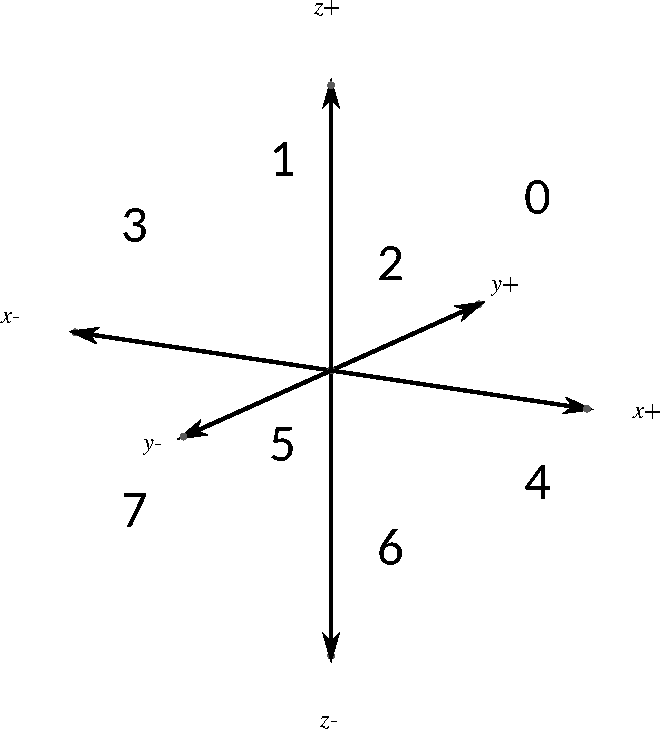
\includegraphics[width=0.7\textwidth,height=\textheight]{040-discretizacion/axes-with-octs.pdf}

}

\caption{image}

\end{figure}

Notamos que el desarrollo binario del índice~\(n\) tiene tres bits y
éstos indican si hubo un cambio de signo o no en cada uno de los tres
ejes con respecto al primer cuadrante, que corresponde a~\(n=0\). De
esta manera, podemos generar las
direcciones~\(\boldsymbol{\hat{\Omega}}_m\)
para~\(m=N(N+2)/8+1, N(N+2)\) a partir de las direcciones del primer
cuadrante~\(\boldsymbol{\hat{\Omega}}_j\) para~\(j=1,N(N+2)/8\) con el
algoritmo de la
figura~\protect\hyperlink{alg:extension}{{[}alg:extension{]}}, donde el
símbolo ampersand~\passthrough{\lstinline!\&!} indica el operador
binario \passthrough{\lstinline!AND!} y el signo de
pregunta~\passthrough{\lstinline!?!} el operador ternario de decisión.
La figura~\protect\hyperlink{fig:latsn}{1.2} muestra el detalle de las
latitudes y longitudes en la esfera unitaria del primer cuadrante y el
conjunto resultante de las \(N(N+2)\) direcciones para~S\(_2\), S\(_4\)
y~\(S_6\) que resultan de aplicar este desarrollo.

\protect\hypertarget{fig:latsn}{}{}Latitudes y longitudes en el primer
cuadrante (izquierda) y conjunto de las~{N(N+2)} direcciones de la
cuadratura de nivel simétrico para~S{2}, S{4} y~{S6} generadas a partir
de un único coseno director positivo~{μ1} de la tabla~1.1, aplicando con
la ecuación~{[}eq:cosenos{]} para obtener el resto de los cosenos
positivos, permutándolos según la tabla~1.2 y extendiéndolos al resto de
los octantes con el algoritmo~{[}alg:extension{]}. Las figuras son
reproducciones tridimensionales realizadas con la herramienta Gmsh a
partir de la información calculada y que realmente utiliza milonga
(capítulo~{[}cap:implementacion{]}) para realizar cálculos de transporte
con el método de las ordenadas discretas.

\hypertarget{sec-dosdimensiones}{%
\subsection{Dos dimensiones}\label{sec-dosdimensiones}}

El caso bidimensional en realidad es un problema en tres dimensiones
pero sin dependencia de los parámetros del problema en una de las
variables espaciales, digamos~\(z\). De esta manera, el dominio~\(U\) de
la geometría está definido sólo sobre el plano~\(x\)-\(y\) y las
direcciones de vuelo~\(\omegaversor\) de los neutrones son simétricas
con respecto a este plano ya que por cada
dirección~\(\omegaversor = [\hat{\Omega}_x \, \hat{\Omega}_y \, \hat{\Omega}_z]\)
con~\(\hat{\Omega}_z>0\) hay una dirección
simétrica~\(\omegaprimaversor = [\hat{\Omega}_x \, \hat{\Omega}_y \, -\hat{\Omega}_z]\)
(figura~\protect\hyperlink{fig:symmetry2d}{1.3}). Luego, las posibles
direcciones se reducen a la mitad, es decir~\(N(N+2)/2\).

\protect\hypertarget{fig:symmetry2d}{}{}Simetría con respecto al
plano~{x}-{y} en un problema bi-dimensional. Por cada
dirección~{\(\omegaversor\)} con componente~{z} positiva (línea llena)
hay una dirección~{\(\omegaprimaversor\)} simétrica e igualmente posible
con~{Ω̂z \textless{} 0} (línea de trazos).

Como la derivada espacial del flujo angular con respecto a~\(z\) es cero
entonces por un lado podemos escribir el término de transporte en la
ecuación~\protect\hyperlink{eq:transportesngeneral}{{[}eq:transportesngeneral{]}}
como

\[\hat{\Omega}_{mx} \cdot \frac{\partial{\psi_{mg}}(x,y)}{\partial x} + \hat{\Omega}_{my} \cdot \frac{\partial{\psi_{mg}(x,y)}}{\partial y}\]
donde ahora~\(m=1,\dots,M = N(N+2)/2\). La componente~\({\Omega}_{mz}\)
no aparece explícitamente en las ecuaciones pero sí lo hace
implícitamente en la elección de las direcciones, ya que siguen siendo
válidas las
ecuaciones~\protect\hyperlink{eq:normalizaciondirecciones}{{[}eq:normalizaciondirecciones{]}}
y~\protect\hyperlink{eq:normalizacionpesos}{{[}eq:normalizacionpesos{]}}.
Esto implica que en cada cuadrante tenemos nuevamente~\(N(N+2)/8\)
direcciones posibles, que luego debemos rotar para obtener las~\(M\)
direcciones en los cuatro cuadrantes. Dado que por un lado los pesos
deben estar normalizados a uno y por otro para cada dirección
con~\(\hat{\Omega}_z>0\) hay otra dirección simétrica
con~\(\hat{\Omega}_z<0\), entonces el conjunto de cuadraturas de nivel
simétrico para el primer cuadrante de un dominio de dos dimensiones
consiste en las mismas~\(N(N+2)/8\) direcciones correspondientes a tres
dimensiones definidas en las
tablas~\protect\hyperlink{tab:quadratureset}{1.1}
y~\protect\hyperlink{tab:mus}{1.2}, cada una con el doble de peso. En
forma equivalente, podemos concluir que las
tablas~\protect\hyperlink{tab:quadratureset}{1.1}
y~\protect\hyperlink{tab:mus}{1.2} valen para dos dimensiones con la
salvedad de que el título de la tercera columna de la
tabla~\protect\hyperlink{tab:quadratureset}{1.1} debe ser~\(4\cdot w_i\)
en lugar de~\(8\cdot w_i\) y debemos reemplazar la palabra ``octante''
por ``cuadrante.'' En la
figura~\protect\hyperlink{fig:direcciones2d}{1.4} mostramos las
direcciones para la cuadratura de nivel simétrico utilizado en este
trabajo para problemas de dos dimensiones espaciales.

\protect\hypertarget{fig:direcciones2d}{}{}Direcciones para el conjunto
de cuadraturas de nivel simétrico en dos dimensiones.

\hypertarget{una-dimensiuxf3n}{%
\subsection{Una dimensión}\label{una-dimensiuxf3n}}

El caso unidimensional es radicalmente diferente a los otros dos. Si
tomamos al eje~\(x\) como la dirección de dependencia espacial, las
posibles direcciones de viaje pueden depender sólo del ángulo
cenital~\(\theta\) ya que la simetría implica que todas las posibles
direcciones azimutales con respecto al eje~\(x\) son igualmente
posibles.

\protect\hypertarget{fig:symmetry1d}{}{}Simetría con respecto al eje~{x}
en un problema unidimensional. Por cada dirección~{\(\omegaversor\)}
(línea llena) hay infinitas direcciones simétricas e igualmente posibles
apuntando en la dirección del círculo subtendido por el
ángulo~{θ = arctan (Ω̂z/Ω̂x)}, representadas por las tres direcciones
primadas (líneas de trazos).

El término de transporte de la
ecuación~\protect\hyperlink{eq:transportesngeneral}{{[}eq:transportesngeneral{]}}
es entonces

\[\hat{\Omega}_{mx} \cdot \frac{\partial{\psi_{mg}}(x)}{\partial x}\]

El hecho de que no una sino dos componentes de~\(\omegaversor\) no
aparezcan explícitamente relaja mucho más las condiciones para la
elección de las~\(M=N\) direcciones. En efecto, la única condición es
simetría completa entre el semieje~\(x>0\) y el semieje~\(x<0\), lo que
nos deja con~\(N/2\) direcciones en cada semieje, todas ellas libres e
independientes.

Para seleccionar las~\(N/2\) direcciones y sus pesos asociados, notamos
que en una dimensión

\[\label{eq:1dgauss}
 \int_{4\pi} f(\omegaversor) \, d\omegaversor = 2\pi \int_{-1}^{1} f(\hat{\Omega}_x) \, d\hat{\Omega}_x \simeq 
2\pi \sum_{m=1}^N w_m \cdot f_m =
4\pi \sum_{m=1}^N \frac{w_m}{2} \cdot f_m =
4\pi \sum_{m=1}^N w_m \cdot f_m\]

Si los puntos~\(\hat{\Omega}_{xm}\) y los pesos~\(w_m=2\cdot w_m\) son
los asociados a la integración de Gauss y~\(f(\hat{\Omega}_x)\) es un
polinomio de orden~\(2N-1\) o menos, entonces la integración es exacta y
la ecuación~xxx deja de ser una aproximación para transformarse en una
igualdad. En la tabla~tabla~\ref{tbl-gauss1d} mostramos el conjunto de
cuadraturas utilizadas para una dimensión, que contiene esencialmente
las abscisas y los pesos de la cuadratura de Gauss.

\begin{table}

\begin{minipage}[t]{\linewidth}

{\centering 

\begin{tabular}[t]{lccc}
\toprule
 & \(m\) & \(\hat{\Omega}_{mx}\) & \(w_m = 2 \cdot w_m\)\\
\midrule
S\(_2\) & 1 & \(\sqrt{\frac{1}{3}}\) & 1\\
S\(_4\) & 1 & \(\sqrt{\frac{3}{7}-\frac{2}{7}\sqrt{\frac{6}{5}}}\) & 0.6521451549\\
 & 2 & \(\sqrt{\frac{3}{7}+\frac{2}{7}\sqrt{\frac{6}{5}}}\) & 0.3478548451\\
S\(_6\) & 1 & 0.2386191860 & 0.4679139346\\
 & 2 & 0.6612093864 & 0.3607615730\\
 & 3 & 0.9324695142 & 0.1713244924\\
S\(_8\) & 1 & 0.1834346424 & 0.3626837834\\
 & 2 & 0.5255324099 & 0.5255324099\\
 & 3 & 0.7966664774 & 0.2223810344\\
 & 4 & 0.9602898564 & 0.1012285363\\
\bottomrule
\end{tabular}

}

\subcaption{\label{tbl-gauss1d-1}Conjuntos de cuadratura para problemas
unidimensionales. Las direcciones~\(\hat{\Omega}_{mx}\) coinciden con
las abscisas de la cuadratura de Gauss. Los pesos~\(w_m\) de ordenadas
discretas son la mitad de los pesos~\(w_m\) de la cuadratura de Gauss.
Las direcciones~\(m=N/2+1,\dots,N\) no se muestran pero se obtienen
como~\(\hat{\Omega}_{N/2+m \, x} = -\hat{\Omega}_{mx}\)
y~\(w_{N/2+m} = w_m\).}
\end{minipage}%

\caption{\label{tbl-gauss1d}\textbf{?(caption)}}

\end{table}

\hypertarget{sec-discretizacion-espacial}{%
\section{Discretización en espacio}\label{sec-discretizacion-espacial}}

Hasta el momento, tenemos por un lado las~\(G\) ecuaciones de difusión
multigrupo

\[\tag{\ref{eq-difusionmultigrupo}}
\begin{gathered}
 - \text{div} \Big[ D_g(\vec{x}) \cdot \text{grad} \left[ \phi_g(\vec{x}) \right] \Big]
 + \Sigma_{t g}(\vec{x}) \cdot \phi_g(\vec{x})
 = \\
\sum_{g^\prime = 1}^G \Sigma_{s_0 g^\prime \rightarrow g}(\vec{x})  \cdot \phi_{g^\prime}(\vec{x}) +
\chi_g \sum_{g^\prime = 1}^G \nu\Sigma_{fg^\prime}(\vec{x}) \cdot \phi_{g^\prime}(\vec{x})+ s_{0g}(\vec{x})
\end{gathered}
\] y las~\(MG\) ecuaciones de transporte~\(S_N\) multigrupo

\[\tag{\ref{eq-transporte-sn}}
\begin{gathered}
 \omegaversor_m \cdot \text{grad} \left[ \psi_{mg}(\vec{x}) \right]  +
 \Sigma_{t g}(\vec{x}) \cdot \psi_{mg}(\vec{x}) =
 \sum_{g=1}^G \Sigma_{s_0 g^\prime \rightarrow g}(\vec{x})  \sum_{m^\prime=1} w_{m^\prime} \psi_{m^\prime g^\prime}(\vec{x})  + \\
 3  \sum_{g=1}^G \Sigma_{s_1 g^\prime \rightarrow g}(\vec{x}) \sum_{m^\prime=1} w_{m^\prime} \left( \omegaversor_{m} \cdot \omegaversor_{m^\prime} \right) \psi_{m^\prime g^\prime}(\vec{x}) +
 \chi_g \sum_{g^\prime=1}^G \nu\Sigma_{fg^\prime}(\vec{x})   \sum_{m^\prime=1} w_{m^\prime} \psi_{m^\prime g^\prime}(\vec{x}) +
s_{mg}(\vec{x})
\end{gathered}
\] en las que las incógnitas~\(\phi_g\) y~\(\psi_{mg}\) dependen
solamente del espacio~\(\vec{x}\). En esta sección empleamos el método
de elementos finitos para discretizar la variable independiente espacial
y obtener finalmente un sistema de ecuaciones algebraicas que nos
permita resolver neutrónica a nivel de núcleo en forma numérica con una
(o más) computadora digital.

Existe una gran cantidad de teoría matemática detrás del método de
elementos finitos para resolver ecuaciones diferenciales a partir de
formulaciones débiles o variacionales. Esencialmente el grueso de la
literatura teórica se centra en probar

\begin{enumerate}
\def\labelenumi{\arabic{enumi}.}
\tightlist
\item
  que la formulación débil (definición~\ref{def-formulacion-debil}) de
  una ecuación diferencial es formalmente correcta con respecto a
  derivabilidad e integrabilidad en el sentido de distribuciones sobre
  espacios de Hilbert,
\item
  que soluciones continuas pero no necesariamente diferenciables en a lo
  más un sub-espacio de medida cero tienen sentido matemático, y
\item
  que el esquema numérico es consistente
  (definición~\ref{def-consistencia}), estable
  (definición~\ref{def-estabilidad}) y convergente
  (definición~\ref{def-convergencia}).
\end{enumerate}

De la misma manera que el~\textbf{?@sec-transporte-difusion}
esencialmente repetimos teoría matemática ya conocida a partir de
diferentes fuente pero amalgamada de forma tal de unificar nomenclaturas
y criterios, en este hacemos lo mismo por cuestiones de consistencia.
Mostramos algunos resultados conocidos y derivamos con algún cierto
nivel de detalle razonable el problema de aproximación de Galerkin a
partir de la formulación débil de un problema en derivadas parciales.
Dejamos la derivación completa incluyendo la teoría de análisis
funcional necesaria para demostrar completamente todos los resultados
del método de elementos finitos en las referencias {[}3{]}, {[}7{]},
{[}8{]}. En la monografía~{[}2{]} escrita durante el plan de formación
de este doctorado se muestra una derivación de la formulación en
elementos finitos de la ecuación de difusión multigrupo de forma menos
formal pero más intuitiva. Incluso se comparan los resultados numéricos
obtenidos con dicha formulación con los obtenidos con una formulación
basada en volúmenes finitos {[}9{]}.

\begin{proposition}[]\protect\hypertarget{prp-fem-fvm}{}\label{prp-fem-fvm}

Si se pudiera intercambiar en toda la literatura existente (y en las
clases y conferencias académicas) la palabra ``elementos'' por
``volúmenes'' (¿tal vez con \passthrough{\lstinline!sed!} siguiendo la
filosofía del~\textbf{?@sec-unix}?) nadie notaría la diferencia. Ver la
referencia~{[}10{]} y sus doscientas ochenta referencias para la
historia detrás del ``método de elementos finitos''.

\end{proposition}

Comenzamos ilustrando la aplicación el método de elementos finitos a un
operador elíptico escalar, en particular a la ecuación de Poisson
generalizada. Para este caso introducimos las ideas básicas de

\begin{enumerate}
\def\labelenumi{\roman{enumi}.}
\tightlist
\item
  la formulación débil o variacional (sección~\ref{sec-poisson}),
\item
  de la aproximación de Galerkin (sección~\ref{sec-galerkin}), y
\item
  de la discretización por elementos finitos (sección~\ref{sec-fem}).
\end{enumerate}

Luego en la~sección~\ref{sec-difusion-multigrupo-fem} aplicamos estas
ideas para obtener las versiones completamente discretizadas de las
ecuaciones de difusión multigrupo, que también son elípticas pero el
problema deja de ser un escalar en cada nodo espacial y su operador no
es simétrico para~\(G>1\). Finalmente en
la~sección~\ref{sec-sn-multigrupo-fem} hacemos lo mismo para transporte
por~\(S_N\) multigrupo. En este caso la incógnita también tiene varios
grados de libertad en cada nodo espacial y además el operador es
parabólico de primer orden y la formulación numérica requiere de un
término de estabilización.

\hypertarget{sec-poisson}{%
\subsection{Ecuación de Poisson generalizada}\label{sec-poisson}}

Comencemos resolviendo la ecuación escalar elíptica de Poisson
generalizada sobre un dominio
espacial~\(D\)-dimensional~\(U \in \mathbb{R}^D\) con condiciones de
contorno de Dirichlet homogéneas en~\(\Gamma_D \in \partial U\) y
condiciones arbitrarias de Neumann en~\(\Gamma_N \in \partial U\) tal
que~\(\Gamma_D \cup \Gamma_N = \partial U\)
y~\(\Gamma_D \cap \Gamma_N = \emptyset\)
(figura~\ref{fig-dominio-pelado}):

\begin{figure}

{\centering 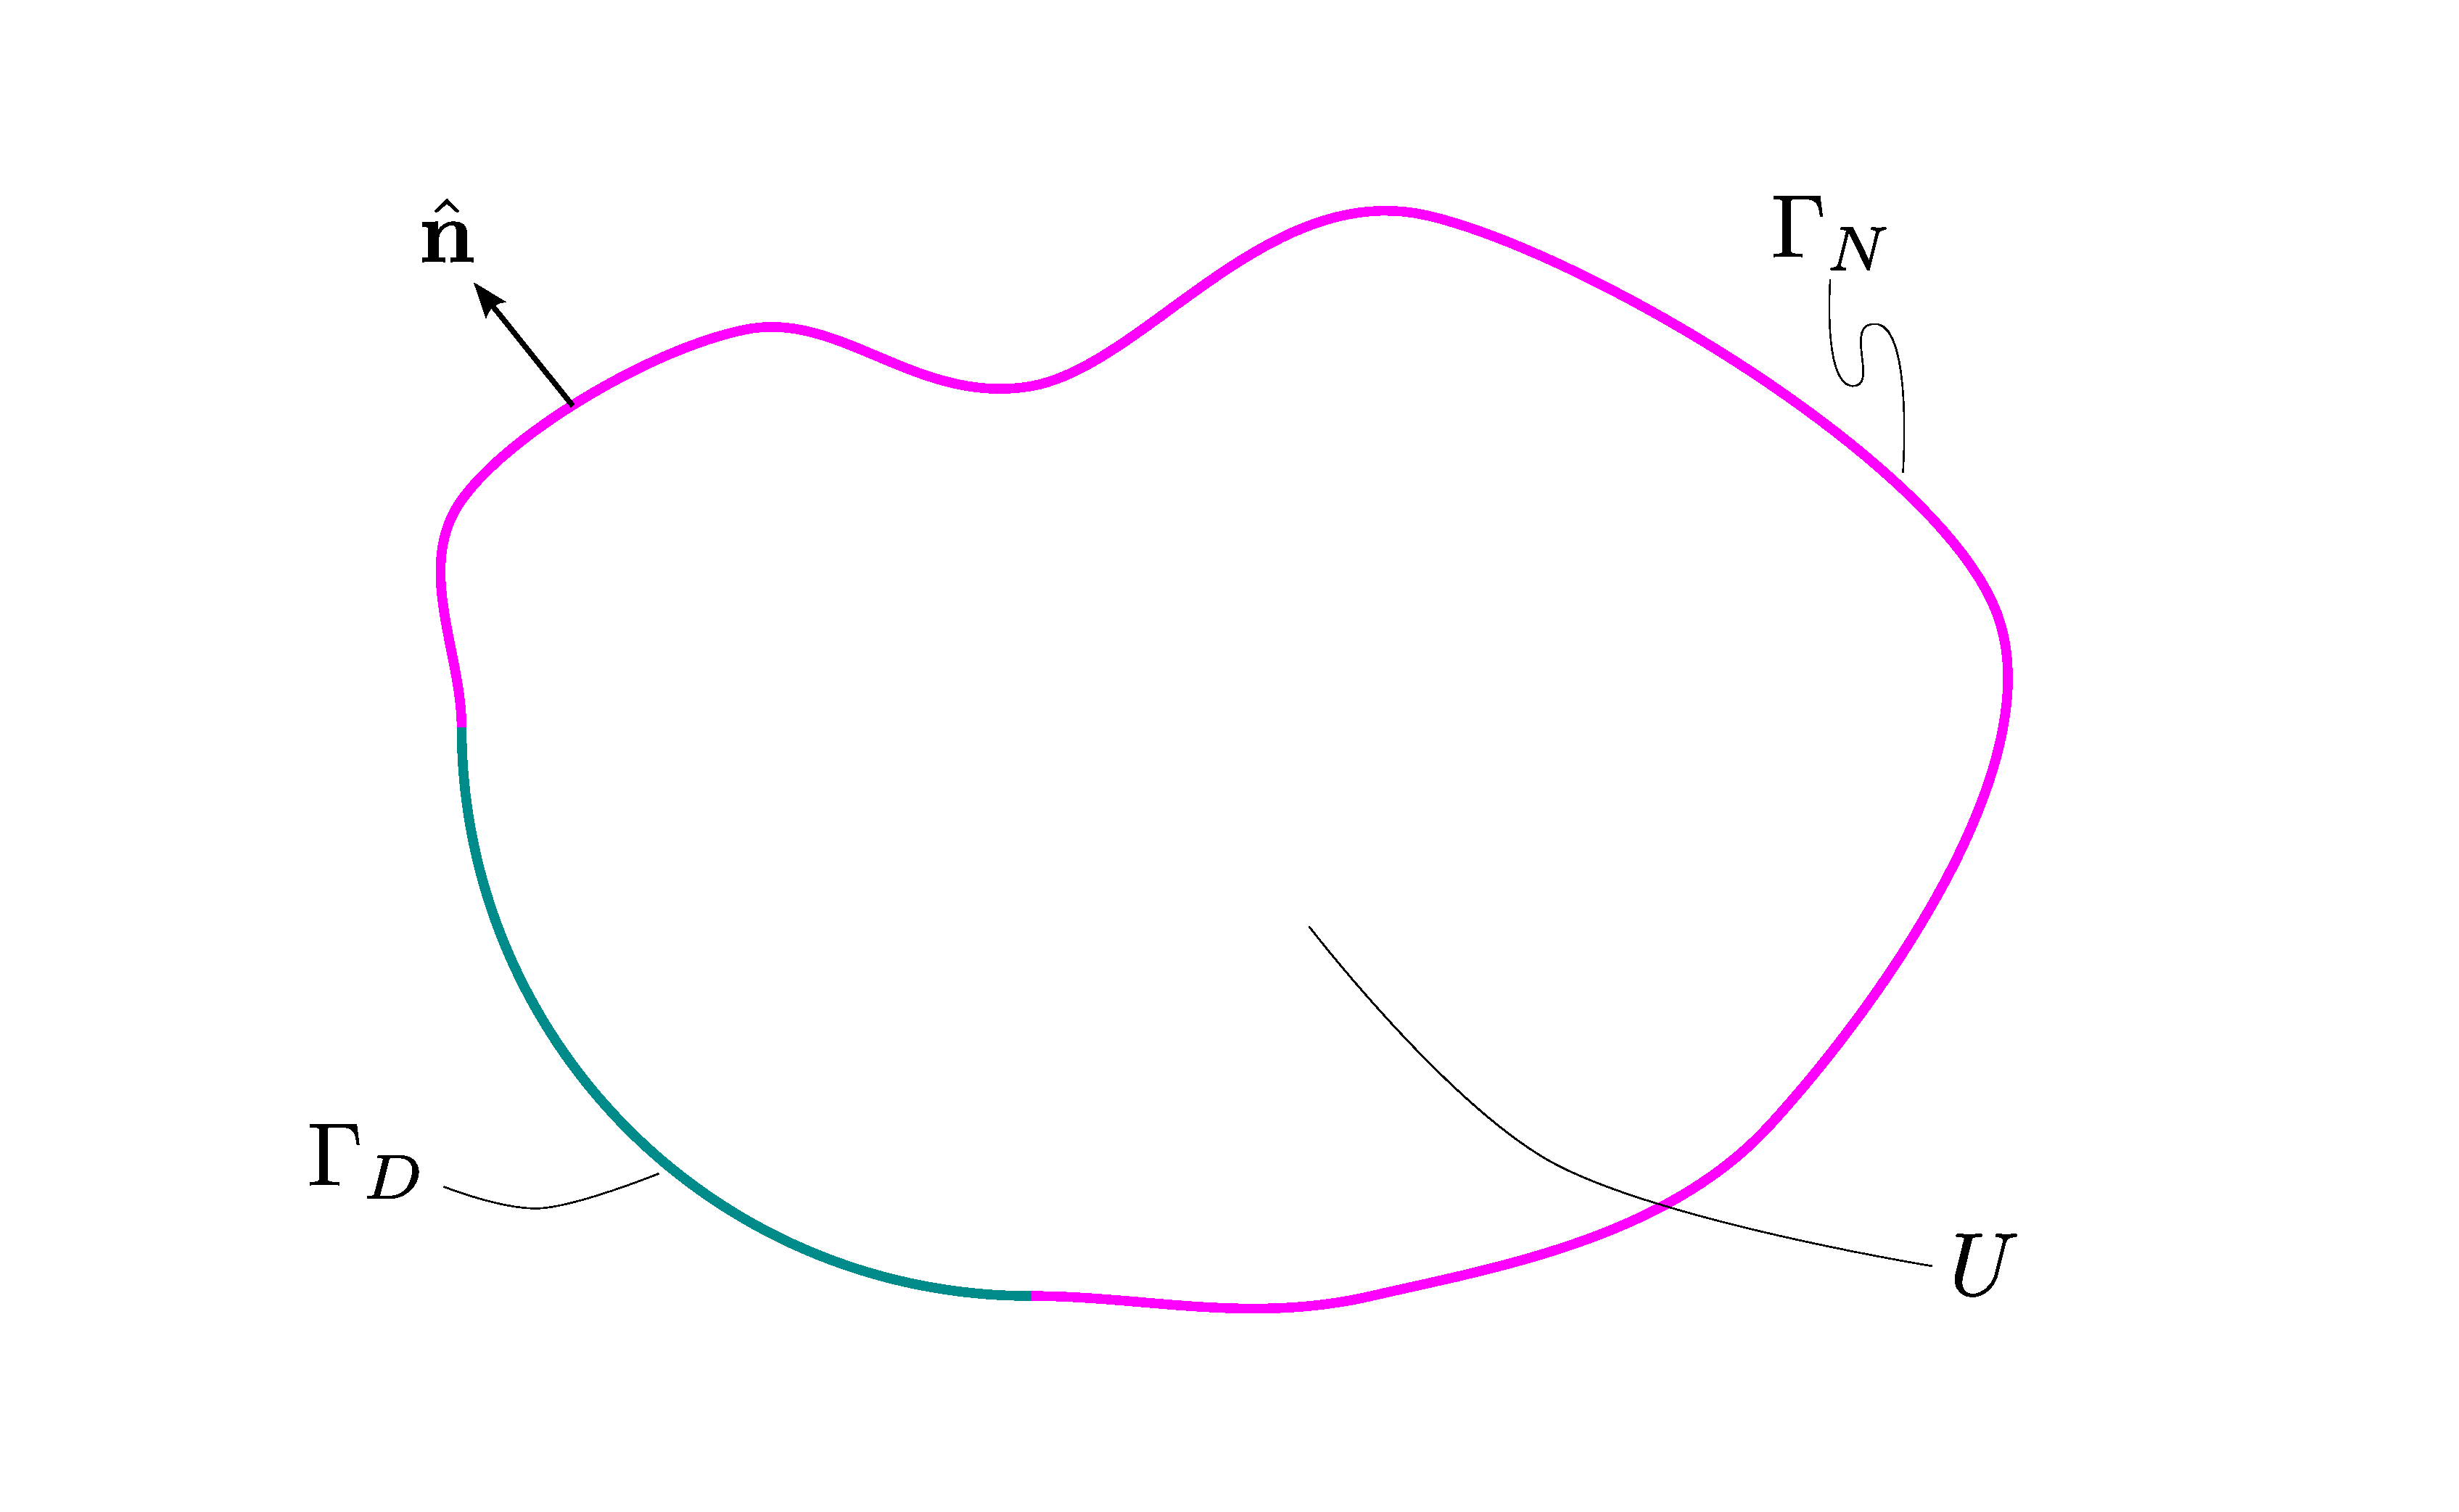
\includegraphics[width=0.75\textwidth,height=\textheight]{040-discretizacion/dominio-pelado.pdf}

}

\caption{\label{fig-dominio-pelado}Un cierto dominio
espacial~\(U \in \mathbb{R}^2\) (bi-dimensional para simplificar la
representación gráfica), con una parte de la frontera~\(\Gamma_D\) con
condiciones de Dirichlet (de color cyan) y otra parte~\(\Gamma_N\) con
condiciones de Neumann (magenta).}

\end{figure}

\begin{equation}\protect\hypertarget{eq-poisson-fuerte}{}{
\begin{cases}
-\text{div} \Big[ k(\vec{x}) \cdot \text{grad} \left[ u(\vec{x}) \right] \Big] = f(\vec{x}) & \forall\vec{x} \in U \\
\hfill u(\vec{x}) = 0 & \forall \vec{x} \in \Gamma_D \\
\hfill k(\vec{x}) \cdot \Big[ \text{grad} \left[ u(\vec{x}) \right] \cdot \hat{\vec{n}} \Big] = p(\vec{x}) & \forall \vec{x} \in \Gamma_N
\end{cases}
}\label{eq-poisson-fuerte}\end{equation} donde \(\hat{\vec{n}}\) es la
normal externa a la frontera~\(\partial U\) en el punto~\(\vec{x}\).

\hypertarget{formulaciones-fuertes-y-duxe9biles}{%
\subsubsection{Formulaciones fuertes y
débiles}\label{formulaciones-fuertes-y-duxe9biles}}

\begin{definition}[formulación
fuerte]\protect\hypertarget{def-formulacion-fuerte}{}\label{def-formulacion-fuerte}

Llamamos a la ecuación diferencial propiamente dicha junto con sus
condiciones de contorno, tal como las escribimos en
la~ecuación~\ref{eq-poisson-fuerte}, la \emph{formulación fuerte} del
problema.

\end{definition}

\begin{remark}

En la formulación fuerte, todas las funciones deben ser derivables al
menos hasta el orden apropiado según dónde aparezca cada una. Por
ejemplo, en la~ecuación~\ref{eq-poisson-fuerte}, \(u\) debe ser
derivable una vez y el producto~\(k \nabla u\) debe ser derivable dos
veces. Este requerimiento usualmente es demasiado restrictivo en
aplicaciones físicas. Por ejemplo, la formulación fuerte del problema de
conducción de calor no está bien definida en las interfaces entre
materiales con diferentes conductividades~\(k\) a cada lado de la
interfaz.

\end{remark}

Multipliquemos ambos miembros de la ecuación diferencial por una cierta
función~\(v(\vec{x})\) que llamamos ``de prueba'':\footnote{Del inglés
  \foreignlanguage{american}{\emph{test funcion}}.}

\begin{equation}\protect\hypertarget{eq-strong-by-u}{}{
 -v(\vec{x}) \cdot \text{div} \Big[ k(\vec{x}) \cdot \text{grad} \left[ u(\vec{x}) \right] \Big] =
 v(\vec{x}) \cdot f(\vec{x})
}\label{eq-strong-by-u}\end{equation}

Esta función de prueba~\(v(\vec{x})\) puede ser (en principio)
arbitraria, pero requerimos que se anule en~\(\Gamma_D\). Es decir, por
ahora pedimos que \(u(\vec{x})\) y~\(v(\vec{x})\) satisfagan las mismas
condiciones de contorno de Dirichlet homogéneas (aunque no
necesariamente las de Neumann).

\begin{theorem}[de la
divergencia]\protect\hypertarget{thm-divergencia}{}\label{thm-divergencia}

En un dominio conexo~\(U \in \mathbb{R}^D\), la integral de volumen
sobre~\(U\) de la divergencia de una función vectorial
continua~\(\vec{F}(\vec{x}) : U \mapsto \mathbb{R}^D\) es igual a la
integral de superficie del producto interno entre~\(\vec{F}\) y la
normal externa~\(\hat{\vec{n}}\) a la frontera~\(\partial U\):

\[
\int_U \mathrm{div} \left[ \vec{F}(\vec{x}) \right] \, d^D\vec{x} =
\int_{\partial U} \vec{F}(\vec{x}) \cdot \hat{\vec{n}} \, d^{D-1}\vec{x}
\]

\begin{proof}

Cualquier libro de Análisis~II.

\end{proof}

\end{theorem}

\begin{corollary}[fórmula de
Green]\protect\hypertarget{cor-green}{}\label{cor-green}

En un dominio conexo~\(U \in \mathbb{R}^D\), sean~\(u(\vec{x})\),
\(v(\vec{x})\) y~\(k(\vec{x})\) funciones continuas
\(U \mapsto \mathbb{R}\). Entonces

\[
\begin{aligned}
\int_U v(\vec{x}) \cdot \mathrm{div} \Big[ k(\vec{x}) \cdot \mathrm{grad} \left[ u(\vec{x}) \right] \Big]  \,d^D\vec{x} =&
-\int_U \mathrm{grad} \left[ v(\vec{x}) \right] \cdot k(\vec{x}) \cdot \mathrm{grad} \left[ u(\vec{x}) \right] \, d^D\vec{x} 
\\
& \quad\quad + \int_{\partial U} v(\vec{x}) \cdot \left[ k(\vec{x}) \cdot \Big( \mathrm{grad}\left[ u(\vec{x}) \right] \cdot \hat{\vec{n}} \Big) \right] \, d^{D-1}\vec{x}
\end{aligned}
\] siendo~\(\hat{\vec{n}}\) la normal exterior a la
frontera~\(\partial U\) en el punto~\(\vec{x}\).

\begin{proof}

Recordando el~\textbf{?@thm-div-inner} de la generalización de la
derivada de un producto que dice que

\[
\text{div} \big[ a \cdot \vec{b} \big ] = a \cdot \text{div} \left[\vec{b}\right] + \vec{b} \cdot \text{grad}\left[a\right]
\] entonces para~\(a = v\) y~\(\vec{b} = k \nabla u\)

\[
\text{div} \Big[ v(\vec{x}) \cdot k(\vec{x}) \cdot \text{grad}\left[ u(\vec{x})\right] \Big] =
v(\vec{x}) \cdot \text{div}\Big[ k(\vec{x}) \cdot \text{grad}\left[ u(\vec{x})\right] \Big] +
k(\vec{x}) \cdot \text{grad}\left[u(\vec{x})\right] \cdot \text{grad}\left[v(\vec{x})\right]
\]

Integrando sobre el volumen~\(U\)\footnote{Llamamos volumen al dominio
  de dimensión~\(D\) y superficie a la frontera de dimensión~\(D-1\).}

\[
\begin{aligned}
\int_U \text{div} \Big[ v(\vec{x}) \cdot k(\vec{x}) \cdot \text{grad}\left[ u(\vec{x})\right] \Big] \, d^D\vec{x} =&
\int_U v(\vec{x}) \cdot \text{div}\Big[ k(\vec{x}) \cdot \text{grad}\left[ u(\vec{x})\right] \Big] \, d^D\vec{x} \\
&\quad +
\int_U k(\vec{x}) \cdot \text{grad}\left[u(\vec{x})\right] \cdot \text{grad}\left[v(\vec{x})\right] \, d^D\vec{x}
\end{aligned}
\]

Haciendo~\(\vec{F}(\vec{x}) = v(\vec{x}) \cdot k(\vec{x}) \cdot \text{grad}\left[ u(\vec{x})\right]\)
en el~teorema~\ref{thm-divergencia} tenemos

\[
\int_U \text{div} \Big[ v(\vec{x}) \cdot k(\vec{x}) \cdot \text{grad}\left[ u(\vec{x})\right] \Big] \, d^D\vec{x} =
\int_{\partial U} v(\vec{x}) \cdot \left[ k(\vec{x}) \cdot \Big( \text{grad}\left[ u(\vec{x}) \right] \cdot \hat{\vec{n}} \Big) \right] \, d^{D-1}\vec{x}
\]

Igualando los miembros derechos de las últimas dos expresiones

\[
\begin{aligned}
\int_{\partial U} v(\vec{x}) \cdot \left[ k(\vec{x}) \cdot \Big( \text{grad}\left[ u(\vec{x}) \right] \cdot \hat{\vec{n}} \Big) \right] \, d^{D-1}\vec{x} =&
\int_U v(\vec{x}) \cdot \text{div}\Big[ k(\vec{x}) \cdot \text{grad}\left[ u(\vec{x})\right] \Big] \, d^D\vec{x} \\
&\quad +
\int_U k(\vec{x}) \cdot \text{grad}\left[u(\vec{x})\right] \cdot \text{grad}\left[v(\vec{x})\right] \, d^D\vec{x}
\end{aligned}
\]

Reordenando los términos, llegamos a la tesis.

\end{proof}

\end{corollary}

Como \(\Gamma_D \cup \Gamma_N = \partial U\)
y~\(\Gamma_D \cap \Gamma_N = \emptyset\), entonces podemos escribir la
integral de superficie sobre la frontera~\(\partial U\) como suma de dos
integrales con el mismo integrando, una sobre~\(\Gamma_D\) y otra
sobre~\(\Gamma_N\):

\[
\begin{aligned}
\int_{\partial U} v(\vec{x}) \cdot \left[ k(\vec{x}) \cdot \Big( \mathrm{grad}\left[ u(\vec{x}) \right] \cdot \hat{\vec{n}} \Big) \right] \, d^{D-1}\vec{x}
=&
\int_{\Gamma_D} v(\vec{x}) \cdot \left[ k(\vec{x}) \cdot \Big( \mathrm{grad}\left[ u(\vec{x}) \right] \cdot \hat{\vec{n}} \Big) \right] \, d^{D-1}\vec{x} \\
&\quad +
\int_{\Gamma_N} v(\vec{x}) \cdot \left[ k(\vec{x}) \cdot \Big( \mathrm{grad}\left[ u(\vec{x}) \right] \cdot \hat{\vec{n}} \Big) \right] \, d^{D-1}\vec{x}
\end{aligned}
\]

Pero

\begin{enumerate}
\def\labelenumi{\roman{enumi}.}
\item
  habíamos pedido que~\(v(\vec{x})\) se anule en~\(\Gamma_D\)

  \[
  v(\vec{x}) = 0 \quad \forall \vec{x} \in \Gamma_D
  \]
\item
  la condición de contorno de Neumann indica que

  \[
  k(\vec{x}) \cdot \Big[ \text{grad} \left[ u(\vec{x}) \right] \cdot \hat{\vec{n}} \Big] = p(\vec{x}) \quad \forall \vec{x} \in \Gamma_N
  \]
\end{enumerate}

por lo que

\[
\int_{\partial U} v(\vec{x}) \cdot \left[ k(\vec{x}) \cdot \Big( \mathrm{grad}\left[ u(\vec{x}) \right] \cdot \hat{\vec{n}} \Big) \right] \, d^{D-1}\vec{x}
 =
\int_{\Gamma_N} v(\vec{x}) \cdot p(\vec{x}) \,d^{D-1}\vec{x}
\]

Volvamos a la~ecuación~\ref{eq-strong-by-u} e integremos ambos miembros
sobre el dominio~\(U\)

\[
-\int_U v(\vec{x}) \cdot \text{div} \Big[ k(\vec{x}) \cdot \text{grad} \left[ u(\vec{x}) \right] \Big]  \,d^D\vec{x}
=
\int_U v(\vec{x}) \cdot f(\vec{x}) \,d^D\vec{x}
\]

Ahora usemos la fórmula de Green y el hecho de que~\(v(\vec{x})\) se
anula en~\(\Gamma_D\) para obtener

\begin{equation}\protect\hypertarget{eq-poisson-debil}{}{
\int_U \text{grad} \left[ v(\vec{x}) \right] \cdot k(\vec{x}) \cdot \text{grad} \left[ u(\vec{x}) \right]  \,d^D\vec{x}
=
\int_U v(\vec{x}) \cdot f(\vec{x}) \,d^D\vec{x}
+ \int_{\Gamma_N} p(\vec{x}) \cdot v(\vec{x}) \,d^{D-1}\vec{x}
}\label{eq-poisson-debil}\end{equation}

\begin{definition}[formulación
débil]\protect\hypertarget{def-formulacion-debil}{}\label{def-formulacion-debil}

Llamamos a la expresión que resulta de

\begin{enumerate}
\def\labelenumi{\arabic{enumi}.}
\tightlist
\item
  multiplicar ambos miembros de la ecuación diferencial por una función
  arbitraria llamada ``de prueba'' que se anula en~\(\Gamma_D\),
\item
  integrar sobre el dominio espacial,
\item
  aplicar fórmulas de cálculo vectorial, y
\item
  reemplazar la condición de contorno de Neumann en las integrales de
  superficie
\end{enumerate}

tal como la~ecuación~\ref{eq-poisson-debil}, junto con los
requerimientos que deben satisfacer tanto la función incógnita como la
función de prueba, la \emph{formulación débil} o \emph{variacional} del
problema. Estrictamente hablando, la formulación débil de una ecuación
diferencial es

\[
\text{encontrar~} u(\vec{x}) \in V: \quad
\mathcal{a} \Big(u(\vec{x}), v(\vec{x})\Big) = \mathcal{B} \Big(v(\vec{x})\Big)
\quad  \forall v(\vec{x}) \in V
\] donde~\(V\) es un espacio funcional apropiado, por ejemplo
el~\(H^1_0(U)\) de las
funciones~\(U \in \mathbb{R}^D \mapsto \mathbb{R}\) cuyo gradiente es de
cuadrado integrable (el superíndice uno) en el dominio~\(U\) y que se
anulan en~\(\Gamma_D\) (el subíndice cero)

\[
V = H^1_0 (U) = \left\{ v \in H^1_0 (U) : \int_U \left( \nabla v \right)^{D} \,d^D\vec{x} < \infty \wedge v(\vec{x}) = 0 \forall \vec{x} \in \Gamma_D  \right\}
\] y los operadores~\(\mathcal{a}(u,v) : V \times V \mapsto \mathbb{R}\)
y~\(\mathcal{B}(v) : V \mapsto \mathbb{R}\) se obtienen a partir de los
cuatro pasos arriba mencionados. En particular, para el problema
generalizado de Poisson de la formulación de
la~ecuación~\ref{eq-poisson-debil}, es

\begin{equation}\protect\hypertarget{eq-a-B-poisson}{}{
\begin{aligned}
\mathcal{a}(u,v) &= \int_U \text{grad}\Big[ v(\vec{x}) \Big] \cdot k(\vec{x}) \cdot \text{grad}\Big[ u(\vec{x}) \Big] \, d^D \vec{x} \\
\mathcal{B}(v) &= \int_U v(\vec{x}) \cdot f(\vec{x}) \, d^D \vec{x} + \int_{\Gamma_N} v(\vec{x}) \cdot p(\vec{x}) \, d^{D-1} \vec{x}
\end{aligned}
}\label{eq-a-B-poisson}\end{equation}

\end{definition}

\begin{remark}

En la formulación débil la derivabilidad es más laxa que en la
formulación fuerte. De ahí su nombre: las funciones deben cumplir
requerimientos más débiles. Por un lado, al involucrar una operación de
integración sobre el dominio y aplicar fórmulas de Green, los
requerimimentos de derivabildiad disminuyen un grado: en la formulación
fuerte~\ref{eq-poisson-fuerte}, \(u\) tiene que ser derivable dos veces
ya que el operador es esencialmente el laplaciano mientras que en la
formulación débil~\ref{eq-poisson-debil} sólo involucra el gradiente. De
hecho, ni siquiera hace falta que las funciones sean tan derivables
según en el lugar dónde aparecen en la formulación ya que las las
integrales deben tomarse según el sentido de Lebesgue y no según el
sentido de como Riemann: todas las funciones dentro de las integrales
pueden ser discontinuas en un sub-espacio de medida nula. En efecto, la
formulación débil del problema de conducción de calor con conductividad
discontinua en interfaces materiales está bien definida. Por un lado las
interfaces materiales son un sub-espacio de medida nula y por otro la
conductividad~\(k(\vec{x})\) no tiene aplicado ningún operador
diferencial sino que es integrado (en el sentido de Lebesgue) sobre el
dominio espacial~\(U\).

\end{remark}

\begin{remark}

La formulación débil de la ecuación de conducción de calor derivada en
la~ecuación~\ref{eq-poisson-debil} incluye la posiblidad de que la
conductividad~\(k(\vec{x})\) pueda depender del espacio e incluso ser
discontinua en interfaces materiales. Más aún, la derivación propuesta
puede ser extendida para el caso no lineal en el cual la conductividad
pueda depender de la incógnita~\(k(u)\).

\textbf{TODO} link a SDS.

\end{remark}

\begin{remark}

El nombre \emph{variacional} viene del hecho de requerir
que~\(\mathcal{a}(u,v) = \mathcal{B}(v)\) para todas las posibles
funciones de prueba~\(v(\vec{x}) \in V\). Es decir, de requerir
que~\(v\) pueda ``variar'' arbitrariamente (siempre que se anule
en~\(\Gamma_D\)) y la igualdad se siga manteniendo.

\end{remark}

\begin{remark}

La formulación fuerte incluye las condiciones de contorno en su
enunciado. Las condiciones de Neumann aparecen naturalmente en los
términos de superficie luego de aplicar las fórmulas de Green y las
condiciones de Dirichlet están esencialmente en el espacio
vectorial~\(V\) donde se busca la solución~\(u\). Las primeras se llaman
\emph{naturales} y las segundas \emph{esenciales}.

\end{remark}

\begin{theorem}[]\protect\hypertarget{thm-equivalencia-fuerte-debil}{}\label{thm-equivalencia-fuerte-debil}

El problema débil es equivalente al fuerte en el sentido de
distribuciones, es decir, ambas formulaciones coinciden excepto en a lo
más un sub-conjunto de~\(U\) de medida cero.

\begin{proof}

Sección~3.3.2 de {[}3{]}, teorema~0.1.4 de {[}7{]} y/o sección~1.4 de
{[}8{]}.

\end{proof}

\end{theorem}

\begin{definition}[funcional
lineal]\protect\hypertarget{def-H-lineal}{}\label{def-H-lineal}

Un funcional~\(\mathcal{B}(v) : V \mapsto \mathbb{R}\) es lineal si

\[
\mathcal{B}(\alpha \cdot v_1 + \beta \cdot v_2) = \alpha \cdot  \mathcal{B}(v_1) + \beta \cdot \mathcal{B}(v_2)
\]

\end{definition}

\begin{definition}[operador
bilineal]\protect\hypertarget{def-a-bilineal}{}\label{def-a-bilineal}

Un operador~\(\mathcal{a}(v,u) : V \times V \mapsto \mathbb{R}\) es
bilineal si

\[
\mathcal{a}(\alpha \cdot v_1 + \beta \cdot v_2, u) = \alpha \cdot \mathcal{a}(v_1,u) + \beta \cdot \mathcal{a}(v_2,u)
\] y \[
\mathcal{a}(v, \alpha \cdot u_1 + \beta \cdot u_2) = \alpha \cdot \mathcal{a}(v,u_1) + \beta \cdot \mathcal{a}(v,u_2)
\]

\end{definition}

\begin{definition}[operador
simétrico]\protect\hypertarget{def-a-simetrico}{}\label{def-a-simetrico}

Un operador~\(\mathcal{a}(v,u)\) es simétrico si

\[
\mathcal{a}(v,u) = \mathcal{a}(u,v)
\]

\end{definition}

\begin{definition}[operador
coercivo]\protect\hypertarget{def-a-simetrico}{}\label{def-a-simetrico}

Un operador~\(\mathcal{a}(v,u) : V \times V \mapsto \mathbb{R}\) es
coercivo si existe una constante~\(\alpha >0\) tal que

\[
\mathcal{a}(v,v) \geq \alpha \cdot || v ||^2_V
\]

\end{definition}

\begin{corollary}[]\protect\hypertarget{cor-norma}{}\label{cor-norma}

Si~\(\mathcal{a}(v,u)\) es coercivo entonces

\[
||v||_{\mathcal{a}} = \sqrt{\mathcal{a}(v,v)}
\] es una norma.

\end{corollary}

\begin{theorem}[]\protect\hypertarget{thm-poisson-coercivo}{}\label{thm-poisson-coercivo}

El operador

\[
\mathcal{a}(u,v) = \int_U \mathrm{grad}\Big[ v(\vec{x}) \Big] \cdot k(\vec{x}) \cdot \mathrm{grad}\Big[ u(\vec{x}) \Big] \, d^D \vec{x}
\] es coercivo si~\(k(\vec{x}) > 0 \forall \vec{x} \in U\).

\begin{proof}

Sección~xxx {[}3{]}

\end{proof}

\end{theorem}

\begin{theorem}[de
Lax-Milgram]\protect\hypertarget{thm-existencia-y-unicidad}{}\label{thm-existencia-y-unicidad}

Dada una formulación débil

\[
\text{encontrar~} u \in V: \quad
\mathcal{a} (u, v) = \mathcal{B} (v)
\quad  \forall v \in V
\] siendo

\begin{enumerate}
\def\labelenumi{\alph{enumi}.}
\tightlist
\item
  \(V\) un subespacio de~\(H^1(U)\),
\item
  \(\mathcal{a} : V \times V \mapsto \mathbb{R}\) un operador continuo,
  bilineal y coercivo, y
\item
  \(\mathcal{B} : V \mapsto \mathbb{R}\) un funcional continuo y lineal
\end{enumerate}

entonces la solución~\(u\) existe y es única.

\begin{proof}

Sección xxx de {[}3{]} o sección de {[}7{]}

\end{proof}

\end{theorem}

\hypertarget{sec-dirichlet-nh}{%
\subsubsection{Condiciones de contorno de Dirichlet no
homogéneas}\label{sec-dirichlet-nh}}

Hasta ahora las condiciones de contorno de Dirichlet han sido iguales a
cero, ya que al pedir que tanto la incógnita~\(u\) como las funciones de
prueba~\(v\) pertenezcan a~\(H^1_0\) podemos

\begin{enumerate}
\def\labelenumi{\arabic{enumi}.}
\tightlist
\item
  satisfacer las condiciones esenciales sobre~\(u\), y
\item
  anular el término de superficie sobre~\(\Gamma_D\) de la fórmula de
  Green
\end{enumerate}

Si el problema a resolver tiene una condición de contorno no homogénea,
digamos

\begin{equation}\protect\hypertarget{eq-no-homogeneo}{}{
\begin{cases}
-\text{div} \Big[ k(\vec{x}) \cdot \text{grad} \left[ u(\vec{x}) \right] \Big] = f(\vec{x}) & \forall\vec{x} \in U \\
\hfill u(\vec{x}) = g(\vec{x}) & \forall \vec{x} \in \Gamma_D \\
\hfill k(\vec{x}) \cdot \Big[ \text{grad} \left[ u(\vec{x}) \right] \cdot \hat{\vec{n}} \Big] = p(\vec{x}) & \forall \vec{x} \in \Gamma_N
\end{cases}
}\label{eq-no-homogeneo}\end{equation} entonces una idea sería pedir
que~\(v \in H^1_0\) pero que \(u \in H^1_g\) tal que

\[
H^1_g (U) = \left\{ v \in H^1_g (U) : \int_U \left( \nabla v \right)^{D} \,d^D\vec{x} < \infty \wedge v(\vec{x}) = g(\vec{x})~\forall \vec{x} \in \Gamma_D  \right\}
\]

Este planteo, además de ser poco elegante al romper la simetría
entre~\(u\) y~\(v\), tiene un problema insalvable: \(H^1_g\) es un
conjunto\footnote{Técnicamente es un
  \foreignlanguage{american}{\emph{affine manifold}}.} pero no un
espacio ya que la suma de dos funciones \(u_1 \in H^1_g\)
y~\(u_2 \in H^1_g\) no están en~\(H^1_g\) sino en~\(H^1_{2g}\). Esto
hace que no podamos escribir fácilmente a la incógnita~\(u\) como una
combinacion lineal de una base, que es lo primero que hacemos en
la~sección~\ref{sec-galerkin} que sigue.

Una alternativa es considerar una función continua~\(u_g \in H^1_g\) y
escribir

\begin{equation}\protect\hypertarget{eq-uh-u-ug}{}{
u_h(\vec{x}) = u(\vec{x}) - u_g(\vec{x})
}\label{eq-uh-u-ug}\end{equation} donde \(u_h \in H^1_0\), es decir, se
anula en~\(\Gamma_D\) (el subíndice~\(h\) quiere decir ``homogénea'').
Si el operador~\(\mathcal{a}\) es bilineal, entonces podemos escribir el
problema

\[
\text{encontrar~} u \in V: \quad
\mathcal{a} \left(u, v\right) = \mathcal{B} \left(v\right)
\quad  \forall v \in V
\] como

\[
\text{encontrar~} u_h \in V: \quad
\mathcal{a} \left(u_h, v\right) = \mathcal{B} \left(v\right) - \mathcal{a} \left(u_g, v\right)
\quad  \forall v \in V
\] donde ahora tanto la incógnita parcial~\(u_h\) como las funciones de
prueba~\(v\) pertenecen a \(V = H^1_0\) y todos los datos del problema
están en el miembro derecho de la igualdad. Podemos obtener la incógnita
original~\(u\) a partir de la~ecuación~\ref{eq-uh-u-ug} como

\[
u(\vec{x}) = u_h(\vec{x}) + u_g(\vec{x})
\]

\begin{remark}

\label{remark-ug}

Si bien este procedimiento es matemáticamente correcto, no parece
sencillo encontrar una función~\(u_g \in H^1_g\) apropiada para una
condición de contorno arbitraria~\(g(\vec{x})\). En
la~sección~\ref{sec-fem} mostramos en un espacio vectorial de dimensión
finita el procedimiento es más sencillo. En
el~\textbf{?@sec-implementacion} que sigue mostramos que la
implementación práctica de este tipo de condiciones de contorno es más
sencilla todavía.

\end{remark}

\textbf{TODO}: condiciones de Robin

\hypertarget{sec-galerkin}{%
\subsubsection{Aproximación de Galerkin}\label{sec-galerkin}}

Usando las ideas desarrolladas en la sección anterior, podemos definir
una discretización espacial muy fácilmente como sigue.

\begin{definition}[problema de
Galerkin]\protect\hypertarget{def-galerkin}{}\label{def-galerkin}

Sea~\(V_N\) un subespacio de~\(V = H^1_0(U)\) de dimensión finita~\(N\).
Llamamos \emph{problema de Galerkin} a

\[
\text{encontrar~} u_N \in V_N: \quad
\mathcal{a} (u_N, v_N) = \mathcal{B} (v_N)
\quad  \forall v_N \in V_N
\]

\end{definition}

Como~\(V_N\) es un espacio vectorial de dimensión~\(N\) entonces podemos
encontrar~\(N\) funciones~\(h_i(\vec{x})\) que formen una base
de~\(V_N\)

\[
V_N = \text{span}\Big\{ h_1(\vec{x}), h_2(\vec{x}), \dots, h_N(\vec{x})\Big\}
\]

En efecto, \(v_N \in V_N\) puede ser escrita como una combinación lineal
de las~\(N\) funciones~\(h_i(\vec{x})\)

\begin{equation}\protect\hypertarget{eq-vn-expansion}{}{
v_N(\vec{x}) = \sum_{i=1}^N v_i \cdot h_i(\vec{x})
}\label{eq-vn-expansion}\end{equation}

Para~\(\mathcal{a}\) bilineal y \(\mathcal{B}\) lineal,

\[
\begin{aligned}
0 &= \mathcal{a} \Big(u_N(\vec{x}), v_N(\vec{x})\Big) - \mathcal{B} \Big(v_N(\vec{x})\Big)\\
0 &= \mathcal{a} \left(u_N(\vec{x}), \sum_{i=1}^N v_i \cdot h_i\left(\vec{x}\right)\right) - \mathcal{B} \left(\sum_{i=1}^N v_i \cdot h_i\left(\vec{x}\right)\right) \\
0 &= \sum_{i=1}^N v_i \cdot \left[ \mathcal{a} \Big(u_N(\vec{x}), h_i\left(\vec{x}\right)\Big) - \mathcal{B} \Big(h_i\left(\vec{x}\right)\Big) \right] \\
\end{aligned}
\]

Como esta igualdad tiene que cumplirse~\(\forall v_N \in V_N\) entonces
cada corchete debe anularse independientemente de~\(v_i\), lo que
implica que

\[
\mathcal{a} \Big(u_N(\vec{x}), h_i\left(\vec{x}\right)\Big) = \mathcal{B} \Big(h_i\left(\vec{x}\right)\Big)
\quad \text{para $i=1,\dots,N$}
\]

De la misma manera, \(u_N \in V_N\) por lo que
\(u_N(\vec{x}) = \sum_{j=1}^N u_j \cdot h_j(\vec{x})\) entonces

\[
\begin{aligned}
\mathcal{a} \Big(\sum_{j=1}^N u_j \cdot h_j(\vec{x}), h_i\left(\vec{x}\right)\Big) &= \mathcal{B} \Big(h_i\left(\vec{x}\right)\Big) \\
\sum_{j=1}^N \mathcal{a} \Big(h_i(\vec{x}), h_j\left(\vec{x}\right)\Big) \cdot u_j  &= \mathcal{B} \Big(h_i\left(\vec{x}\right)\Big)
\quad \text{para $i=1,\dots,N$} 
\end{aligned}
\] que podemos escribir en forma matricial como

\begin{equation}\protect\hypertarget{eq-Au}{}{
\mat{A} \cdot \vec{u} = \vec{b}
}\label{eq-Au}\end{equation} siendo

\[
\mat{A} =
\begin{bmatrix}
\mathcal{a}(h_1,h_1) & \mathcal{a}(h_1,h_2) & \cdots & \mathcal{a}(h_1,h_j) & \cdots & \mathcal{a}(h_1,h_N) \\
\mathcal{a}(h_2,h_1) & \mathcal{a}(h_2,h_2) & \cdots & \mathcal{a}(h_2,h_j) & \cdots & \mathcal{a}(h_2,h_N) \\
\vdots               & \vdots               & \ddots & \vdots               & \ddots & \vdots \\
\mathcal{a}(h_i,h_1) & \mathcal{a}(h_i,h_2) & \cdots & \mathcal{a}(h_i,h_j) & \cdots & \mathcal{a}(h_i,h_N) \\
\vdots               & \vdots               & \ddots & \vdots               & \ddots & \vdots \\
\mathcal{a}(h_N,h_1) & \mathcal{a}(h_N,h_2) & \cdots & \mathcal{a}(h_N,h_j) & \cdots & \mathcal{a}(h_N,h_N) \\
\end{bmatrix}
\]

\[
\vec{u} = 
\begin{bmatrix}
u_1 \\
u_2 \\
\vdots \\
u_i \\
\vdots \\
u_N \\
\end{bmatrix}
\quad\quad\quad\quad
\vec{b} = 
\begin{bmatrix}
\mathcal{B}(h_1) \\
\mathcal{B}(h_2) \\
\vdots \\
\mathcal{B}(h_i) \\
\vdots \\
\mathcal{B}(h_N) \\
\end{bmatrix}
\]

\begin{corollary}[]\protect\hypertarget{cor-A-simetria}{}\label{cor-A-simetria}

Si el operador~\(\mathcal{a}\) es simétrico entonces la
matriz~\(\mat{A}\) también es simétrica.

\end{corollary}

\begin{theorem}[]\protect\hypertarget{thm-A-spd}{}\label{thm-A-spd}

Si el operador~\(\mathcal{a}\) es bilineal y coercivo entonces la
matriz~\(\mat{A}\) es definida positiva.

\begin{proof}

\[
\begin{aligned}
\vec{v}^T \cdot \mat{A} \cdot \vec{v}
&= \sum_{i=1}^N \sum_{j=1}^N v_i \cdot \mathcal{a}(h_i, h_j) \cdot v_j \\
&= \sum_{i=1}^N \sum_{j=1}^N \mathcal{a}(v_i \cdot h_i, v_j \cdot h_j) \\
&= \mathcal{a} \left( \sum_{i=1}^N v_i \cdot h_i, \sum_{j=1}^N v_j \cdot h_j\right) \\
&= \mathcal{a}(v_N, v_N) \geq \alpha\cdot ||v_N||_V^2 \geq 0
\end{aligned}
\] para~\(\alpha > 0\). Dado que~ \(||v_N||_V\) es una norma, la
igualdad se cumple si y sólo si~\(||v_N||_V = 0\), lo que implica que
todos los elementos de~\(v\) son nulos.

\textbf{TODO} demostración alternativa de {[}8{]}

\end{proof}

\end{theorem}

\begin{theorem}[existencia y
unicidad]\protect\hypertarget{thm-galerkin-existencia-y-unicidad}{}\label{thm-galerkin-existencia-y-unicidad}

Si el operador~\(\mathcal{a}\) es bilineal y coercivo entonces el
problema de Galerkin de la~definición~\ref{def-galerkin} existe y es
único.

\begin{proof}

Por el~teorema~\ref{thm-A-spd} la matriz~\(\mat{A}\) es definida
positiva. Luego es invertible y
la~ecuación~\ref{eq-Au}~\(\mat{A} \cdot \vec{u} = \vec{b}\) tiene
solución única.

\end{proof}

\end{theorem}

\begin{theorem}[estabilidad]\protect\hypertarget{thm-galerkin-estabilidad}{}\label{thm-galerkin-estabilidad}

El método de Galerkin es estable con respecto a~\(N\).

\begin{proof}

Sección~4.2.2 de~{[}3{]}.

\end{proof}

\end{theorem}

\begin{theorem}[consistencia]\protect\hypertarget{thm-galerkin-consistencia}{}\label{thm-galerkin-consistencia}

El método de Galerkin es fuertemente consistente, es decir

\[
\mathcal{a}(u - u_N, v_N) = 0 \quad \forall v_N \in V_N
\]

\begin{proof}

Como~\(u_N\) es una solución del problema de Galerkin entonces

\[
\mathcal{a}(u_N, v_N) = \mathcal{B}(v_N) \quad \forall v_N \in V_N
\]

Dado que~\(V_N \subset V\) entonces la solución continua~\(u \in V\)
también satisface

\[
\mathcal{a}(u, v_N) = \mathcal{B}(v_N) \quad \forall v_N \in V_N
\]

Restando miembro a miembro

\[
\mathcal{a}(u_N, v_N) - \mathcal{a}(u, v_N) = 0
\] de donde se sigue la tesis por la bilinealidad.

\end{proof}

\end{theorem}

\begin{remark}

El error~\(u - u_N\) cometido por la aproximación de Galerkin es
ortogonal al subespacio~\(V_N\) en la norma

\[
||v||_{\mathcal{a}} = \sqrt{\mathcal{a}(v,v)}
\] Es decir, la solución aproximada~\(u_N\) es

\begin{enumerate}
\def\labelenumi{\arabic{enumi}.}
\tightlist
\item
  La proyección ortogonal de la solución exacta~\(u\) en el
  subespacio~\(V_N\).
\item
  La solución que minimiza la distancia \(||u -u_N||_{\mathcal{a}}\).
\end{enumerate}

\end{remark}

\begin{corollary}[convergencia]\protect\hypertarget{cor-galerkin-convergencia}{}\label{cor-galerkin-convergencia}

Si \(V_N \rightarrow V\) para \(N \rightarrow \infty\) entonces el
método de Galerkin converge a la solución real~\(u\).

\end{corollary}

\begin{remark}

En esta~sección~\ref{sec-poisson} se ha comenzado con la formulación
fuerte de la ecuación diferencial (ecuación~\ref{eq-poisson-fuerte}) y
se ha llegado a un sistema lineal de ecuaciones algebraica
(ecuación~\ref{eq-Au}), pasando por la formulación débil
(definición~\ref{def-formulacion-debil}) y por la aproximación de
Galerkin (definición~\ref{def-galerkin}):

\[
\text{formulación fuerte} \quad \equiv \quad
\text{formulación débil}  \quad \approxident \quad
\text{aproximación de Galerkin} \equiv \quad 
\mat{A} \cdot \vec{u} = \vec{b}
\]

La primera equivalencia está probada por
el~teorema~\ref{thm-equivalencia-fuerte-debil}. No hay ninguna
aproximación, excepto el hecho de que la equivalencia se mantiene en
todo el dominio~\(U\) excepto en, a lo más, un sub-conjunto de medida
cero. La aproximación entre la formulación débil y el problema de
Galerkin es la idea central del método numérico: pasar de una espacio
vectorial~\(V\) de dimensión infinita a un espacio vectorial~\(V_N\) de
dimensión finita. La equivalencia entre Galerkin y un sistema lineal de
ecuaciones algebraicas (que puede ser resuelto con una computadora
digital) funciona siempre y cuando el operador~\(a(u,v)\) sea coercivo y
bilineal. Para problemas no lineales (por ejemplo para el caso en el
que~\(k\) dependiera de~\(u\)) la última equivalencia se reemplaza por
una formulación vectorial no lineal \(\vec{F}(\vec{u})=0\). En
la~sección~\ref{sec-nomult-src} mencionamos brevemente cómo formular y
resolver este tipo de problemas.

\end{remark}

\hypertarget{sec-fem}{%
\subsubsection{Elementos finitos}\label{sec-fem}}

Tomemos un dominio~\(U\in \mathbb{R}^D\) y consideremos~\(J\)
puntos~\(\vec{x}_j \in U\). Estos puntos~\(\vec{x}_i\) para
\(j=1,\dots,J\) incluyen la frontera~\(\Gamma_N\) con condiciones de
contorno de Neumann pero no incluyen a~\(\Gamma_D\) con condiciones de
Dirichlet. Por ejemplo, en la~figura~\ref{fig-dominio-solo-nodos}
tenemos~\(J=32\). Supongamos que existen~\(J\)
funciones~\(h_j(\vec{x})\) ``de forma''\footnote{En la gran mayoría de
  la literatura de elementos finitos las funciones de forman se
  llaman~\(N(\vec{x})\). Como este símbolo no nos parece apropiado para
  una función del espacio, seguimos la nomenclatura de Bathe~{[}11{]}
  (que fue director de doctorado del Dr.~Dvorkin que a su vez organizó
  el departamento de cálculo de la UBA donde este doctorando cursó la
  materia de elementos finitos) que utiliza la
  nomenclatura~\(h(\vec{x})\) para las funciones de forma.} que cumplen
simultáneamente

\begin{equation}\protect\hypertarget{eq-forma-delta-0}{}{
\begin{cases}
h_j(\vec{x}_i) = \delta_{ji} \\
h_j(\vec{x}) = 0 \quad \forall \vec{x} \in \Gamma_D
\end{cases}
}\label{eq-forma-delta-0}\end{equation}

\begin{figure}

{\centering 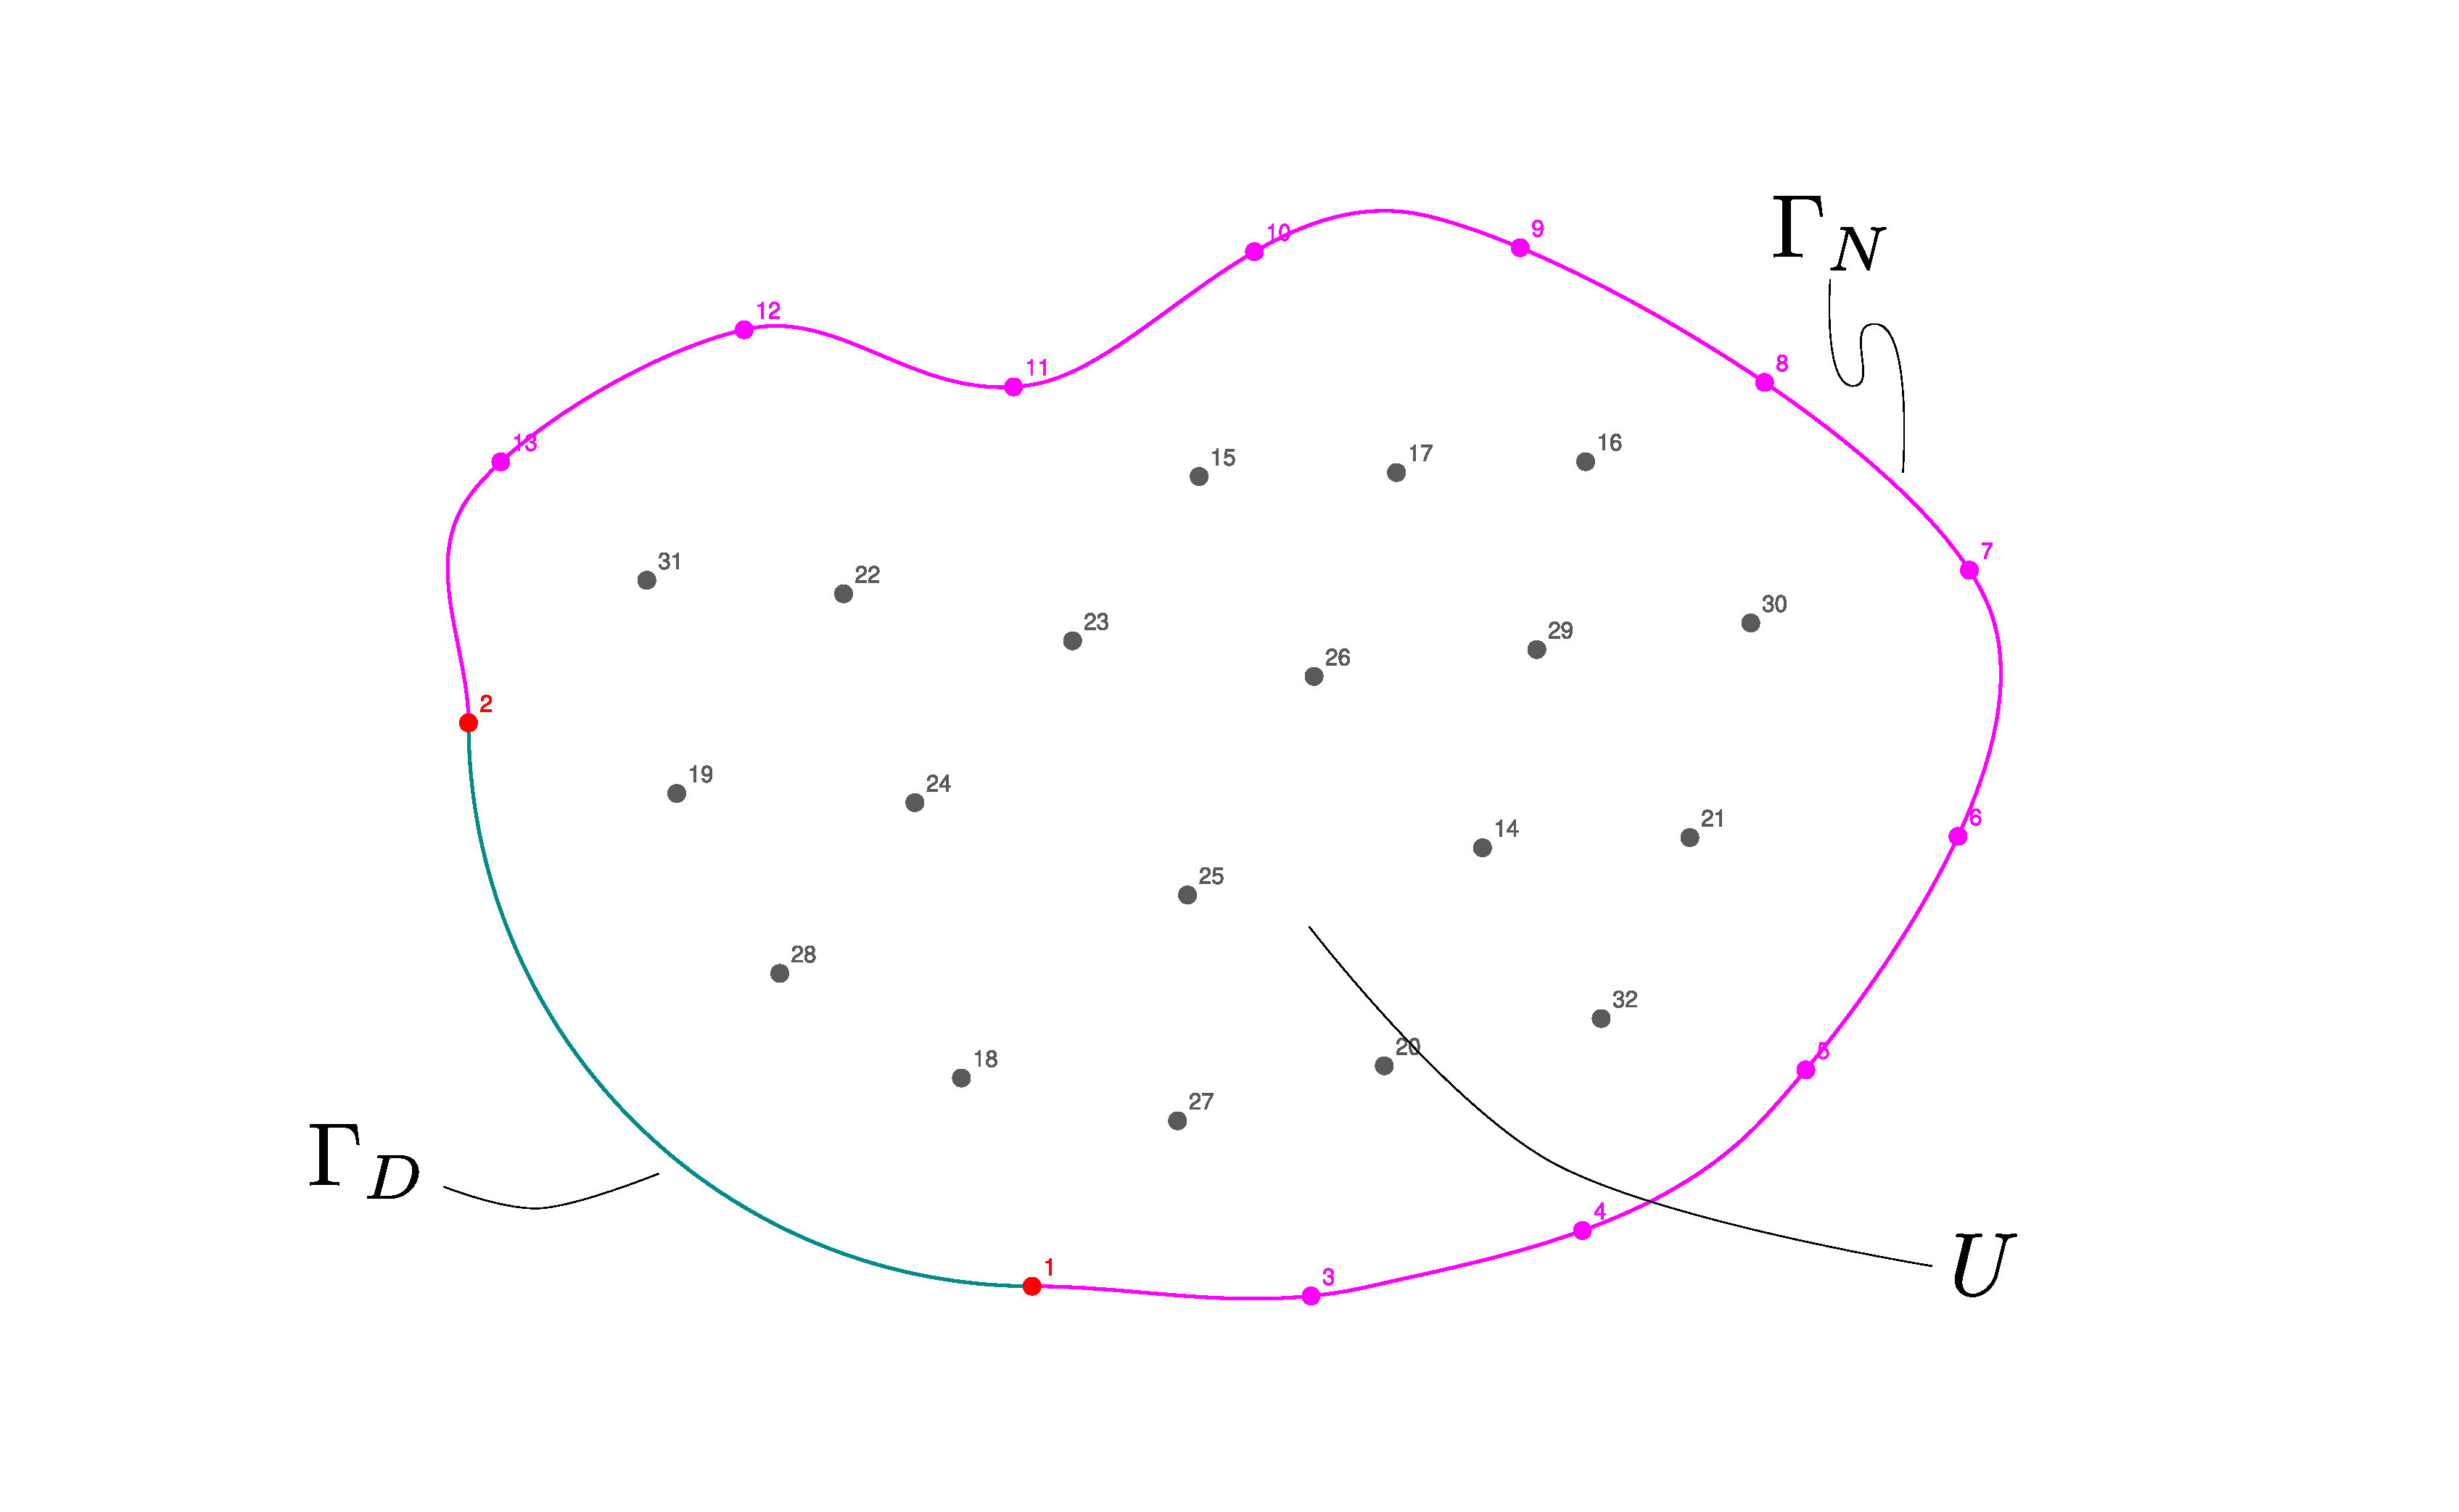
\includegraphics[width=0.75\textwidth,height=\textheight]{040-discretizacion/dominio-solo-nodos.pdf}

}

\caption{\label{fig-dominio-solo-nodos}El dominio espacial~\(U\) de la
\textbf{?@fig-dominio} con \(J=32\) puntos ubicados en la
frontera~\(\Gamma_N\) (\(j=1,\dots,13\)) y en el interior
(\(j=14,\dots,32\)). La frontera~\(\Gamma_D\) con condiciones de
contorno de Dirichlet no tiene ningún punto.}

\end{figure}

Sea~\(V_J\) el espacio vectorial de dimensión~\(J\) generado por
estas~\(J\) funciones de forma~\(h_j(\vec{x})\). Como ya hicimos en
la~ecuación~\ref{eq-vn-expansion}, escribimos a una cierta
función~\(v(\vec{x}) \in V_J\) como una combinación lineal de los
elementos de la base

\begin{equation}\protect\hypertarget{eq-v-vjhj}{}{
v(\vec{x}) = \sum_{j=1}^J v_j \cdot h_j(\vec{x})
}\label{eq-v-vjhj}\end{equation}

Podemos escribir esta expansión en forma matricial como

\[
v(\vec{x}) = \mat{H}(\vec{x}) \cdot \vec{v} = \vec{v}^T \cdot \mat{H}^T(\vec{x})
\] con

\begin{equation}\protect\hypertarget{eq-H}{}{
\mat{H}(\vec{x}) =
\begin{bmatrix}
h_1(\vec{x}) & h_2(\vec{x}) & \cdots & h_j(\vec{x}) & \cdots & h_J(\vec{x})
\end{bmatrix}
}\label{eq-H}\end{equation} y \[
\vec{v} = 
\begin{bmatrix}
v_1 \\
v_2 \\
\vdots \\
v_j \\
\vdots \\
v_J \\
\end{bmatrix}
\]

De la misma forma, el gradiente~\(\nabla v\) es

\[
\text{grad} \Big[ v(\vec{x}) \Big] =
\begin{bmatrix}
\displaystyle\frac{\partial v}{\partial x} \\
\displaystyle\frac{\partial v}{\partial y} \\
\displaystyle\frac{\partial v}{\partial z}
\end{bmatrix}
=
\begin{bmatrix}
\displaystyle \sum_{j=1}^J v_j \cdot \frac{\partial h_j}{\partial x} \\
\displaystyle \sum_{j=1}^J v_j \cdot \frac{\partial h_j}{\partial y} \\
\displaystyle \sum_{j=1}^J v_j \cdot \frac{\partial h_j}{\partial z}
\end{bmatrix}
=
\mat{B}(\vec{x}) \cdot \vec{v}
=
\vec{v}^T \cdot \mat{B}^T(\vec{x})
\] con

\begin{equation}\protect\hypertarget{eq-B}{}{
\mat{B}(\vec{x}) =
\begin{bmatrix}
\displaystyle \frac{\partial h_1}{\partial x} & \displaystyle \frac{\partial h_2}{\partial x} & \cdots & \displaystyle \frac{\partial h_j}{\partial x} & \cdots & \displaystyle \frac{\partial h_J}{\partial x} \\
\displaystyle \frac{\partial h_1}{\partial y} & \displaystyle \frac{\partial h_2}{\partial y} & \cdots & \displaystyle \frac{\partial h_j}{\partial y} & \cdots & \displaystyle \frac{\partial h_J}{\partial y} \\
\displaystyle \frac{\partial h_1}{\partial z} & \displaystyle \frac{\partial h_2}{\partial z} & \cdots & \displaystyle \frac{\partial h_j}{\partial z} & \cdots & \displaystyle \frac{\partial h_J}{\partial z} \\
\end{bmatrix}
}\label{eq-B}\end{equation}

Reemplazando la forma particular del operador~\(\mathcal{a}\) y del
funcional~\(\mathcal{B}\) para el problema generalizado de Poisson de
la~ecuación~\ref{eq-a-B-poisson}, tenemos

\[
\begin{aligned}
\mathcal{a}(u,v) &= \int_U \text{grad}\Big[ v(\vec{x}) \Big] \cdot k(\vec{x}) \cdot \text{grad}\Big[ u(\vec{x}) \Big] \, d^D \vec{x} \\ 
&= \int_U \vec{v}^T \cdot \mat{B}^T(\vec{x}) \cdot k(\vec{x}) \cdot \mat{B}(\vec{x}) \cdot \vec{u} \,\, d^D\vec{x} \\
&= \vec{v}^T \cdot \left[ \int_U \mat{B}^T(\vec{x}) \cdot k(\vec{x}) \cdot \mat{B}(\vec{x}) \, d^D\vec{x} \right] \cdot \vec{u} \\
\end{aligned}
\]

\[
\begin{aligned}
\mathcal{B}(v) &= \int_U v(\vec{x}) \cdot f(\vec{x}) \, d^D \vec{x} + \int_{\Gamma_N} v(\vec{x}) \cdot p(\vec{x}) \, d^{D-1} \vec{x} \\
&= \int_U \vec{v}^T \cdot \mat{H}^T(\vec{x}) \cdot f(\vec{x}) \, d^D \vec{x}
+ \int_{\Gamma_N} \vec{v}^T \cdot \mat{H}^T(\vec{x}) \cdot p(\vec{x}) \, d^{D-1} \vec{x} \\
&= \vec{v}^T \cdot \left[ \int_{U} \mat{H}^T(\vec{x}) \cdot f(\vec{x}) \, d^D \vec{x}
+ \int_{\Gamma_N} \mat{H}^T(\vec{x}) \cdot p(\vec{x}) \, d^{D-1}\vec{x} \right]
\end{aligned}
\]

Como \(\mathcal{a}(u,v) = \mathcal{B}(v) \quad \forall v \in V_J\)
entonces llegamos otra vez a

\[
\mat{A} \cdot \vec{u} = \vec{b}
\] donde ahora tenemos una representación explícita particular
para~\(\mat{A} \in \mathbb{R}^{J \times J}\)
y~\(\vec{u} \in \mathbb{R}^J\) a partir de las
ecuaciones~{[}-ecuación~\ref{eq-H}\} y~\ref{eq-B} como

\begin{equation}\protect\hypertarget{eq-A-b-poisson}{}{
\begin{aligned}
\mat{A} &= \int_U \mat{B}^T(\vec{x}) \cdot k(\vec{x}) \cdot \mat{B}(\vec{x}) \, d^D\vec{x} \\
\vec{b} &= \int_{\Gamma_N} \mat{H}^T(\vec{x}) \cdot p(\vec{x}) \, d^{D-1} \vec{x}
+ \int_{\Gamma_N} \mat{H}^T(\vec{x}) \cdot p(\vec{x}) \, d^{D-1}\vec{x}
\end{aligned}
}\label{eq-A-b-poisson}\end{equation}

Una vez más, tal como hemos dicho en la observación sobre la
construcción de la función~\(u_g\) necesaria para satisfacer condiciones
de contorno de Dirichlet no homogéneas de la página~\pageref{remark-ug},
estas últimas dos expresiones son correctas. Pero no parece
sencillo\ldots{}

\label{dos}

\begin{enumerate}
\def\labelenumi{\arabic{enumi}.}
\tightlist
\item
  encontrar las~\(J\) funciones de forma~\(h_j(\vec{x})\) adecuadas que
  cumplan las condiciones~\ref{eq-forma-delta-0} (como por ejemplo las
  ilustradas en la figura~\ref{fig-shape-function-first-order}), ni
\item
  calcular las integrales para obtener la
  matriz~\(\mat{A} \in \mathbb{R}^{J \times J}\) y el
  vector~\(\vec{b} \in \mathbb{R}^J\).
\end{enumerate}

\begin{figure}

\begin{minipage}[t]{0.47\linewidth}

{\centering 

\raisebox{-\height}{

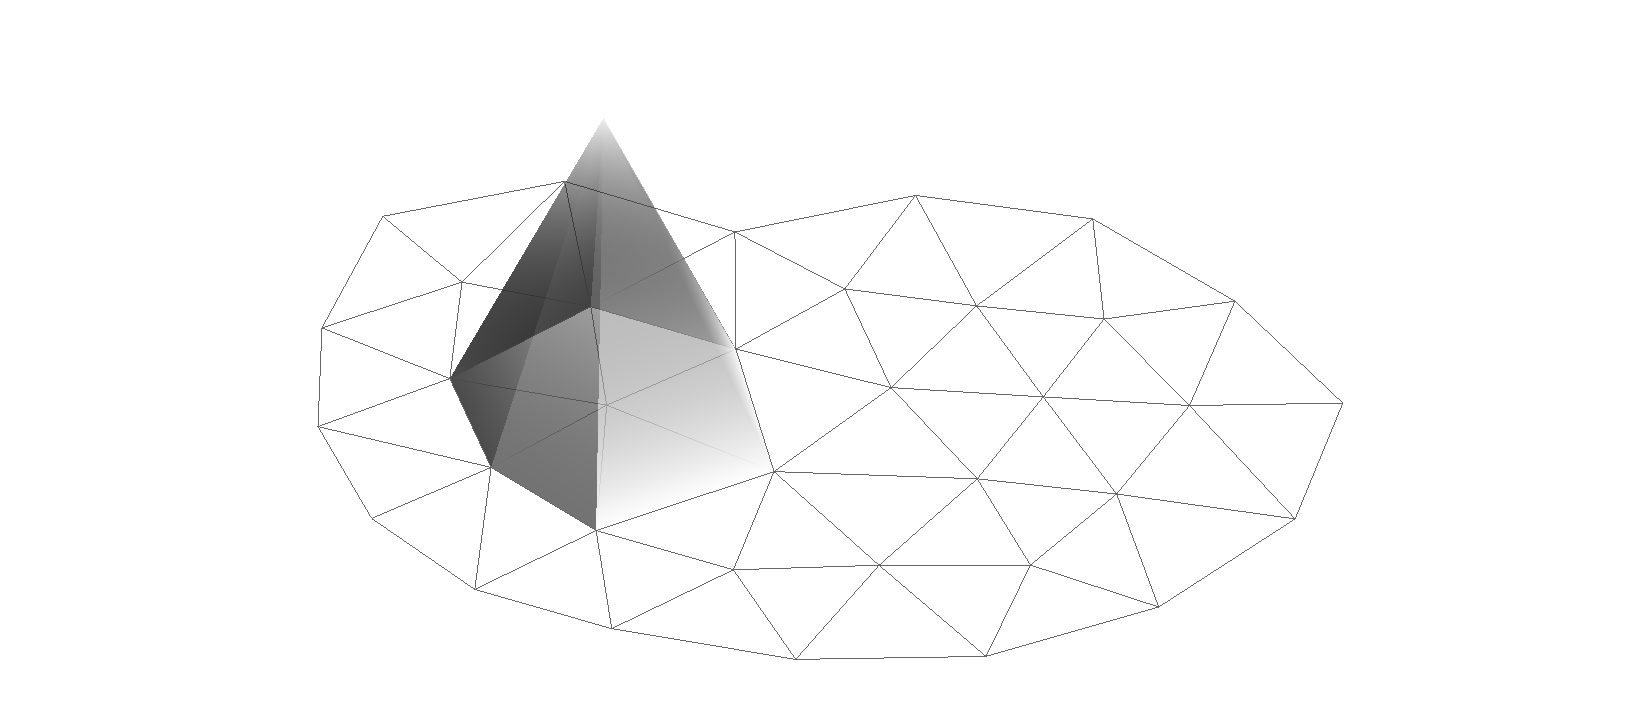
\includegraphics{040-discretizacion/shape-function-first-order-24.png}

}

}

\subcaption{\label{fig-shape-function-first-order-24}\(h_{24}(\vec{x})\)}
\end{minipage}%
%
\begin{minipage}[t]{0.05\linewidth}

{\centering 

~

}

\end{minipage}%
%
\begin{minipage}[t]{0.47\linewidth}

{\centering 

\raisebox{-\height}{

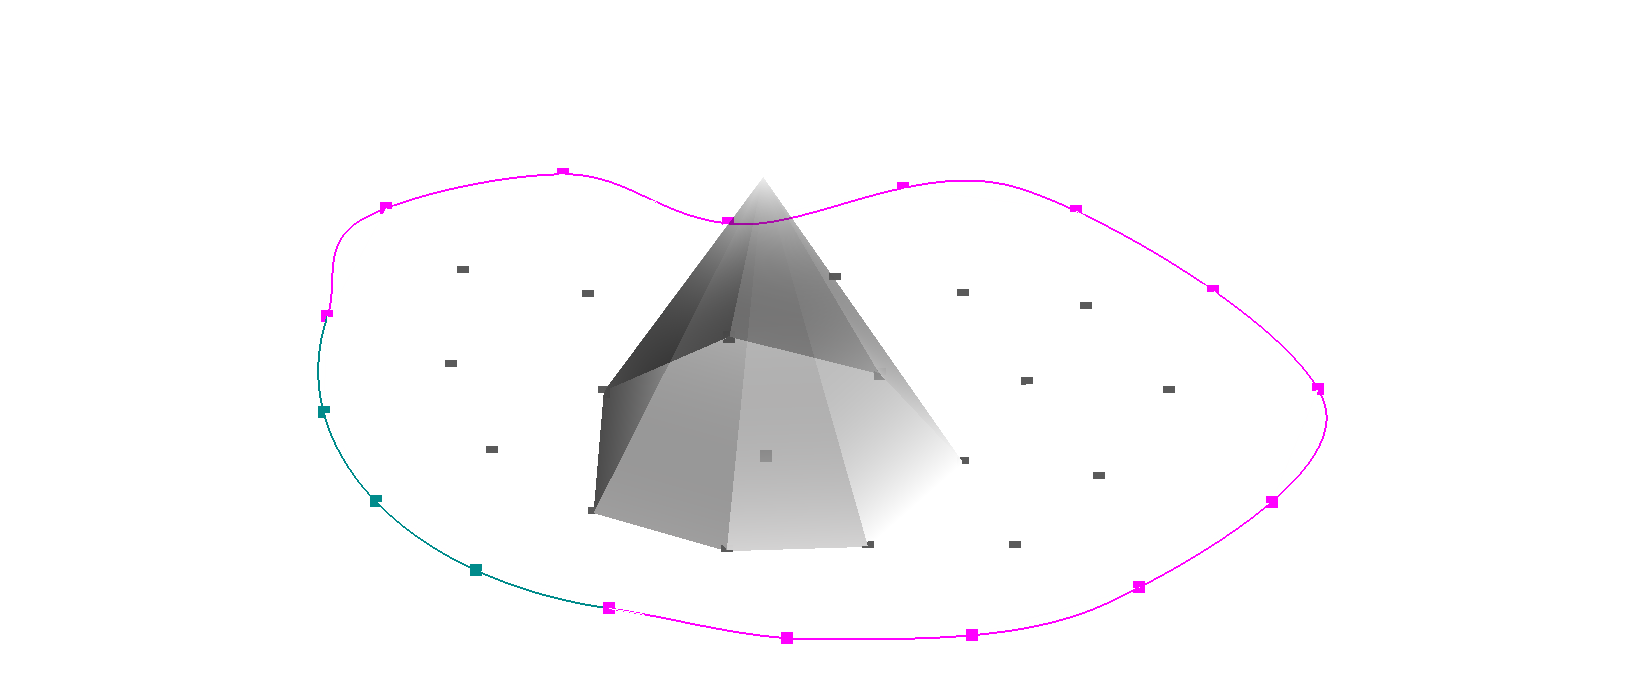
\includegraphics{040-discretizacion/shape-function-first-order-25.png}

}

}

\subcaption{\label{fig-shape-function-first-order-25}\(h_{25}(\vec{x})\)}
\end{minipage}%
\newline
\begin{minipage}[t]{0.47\linewidth}

{\centering 

\raisebox{-\height}{

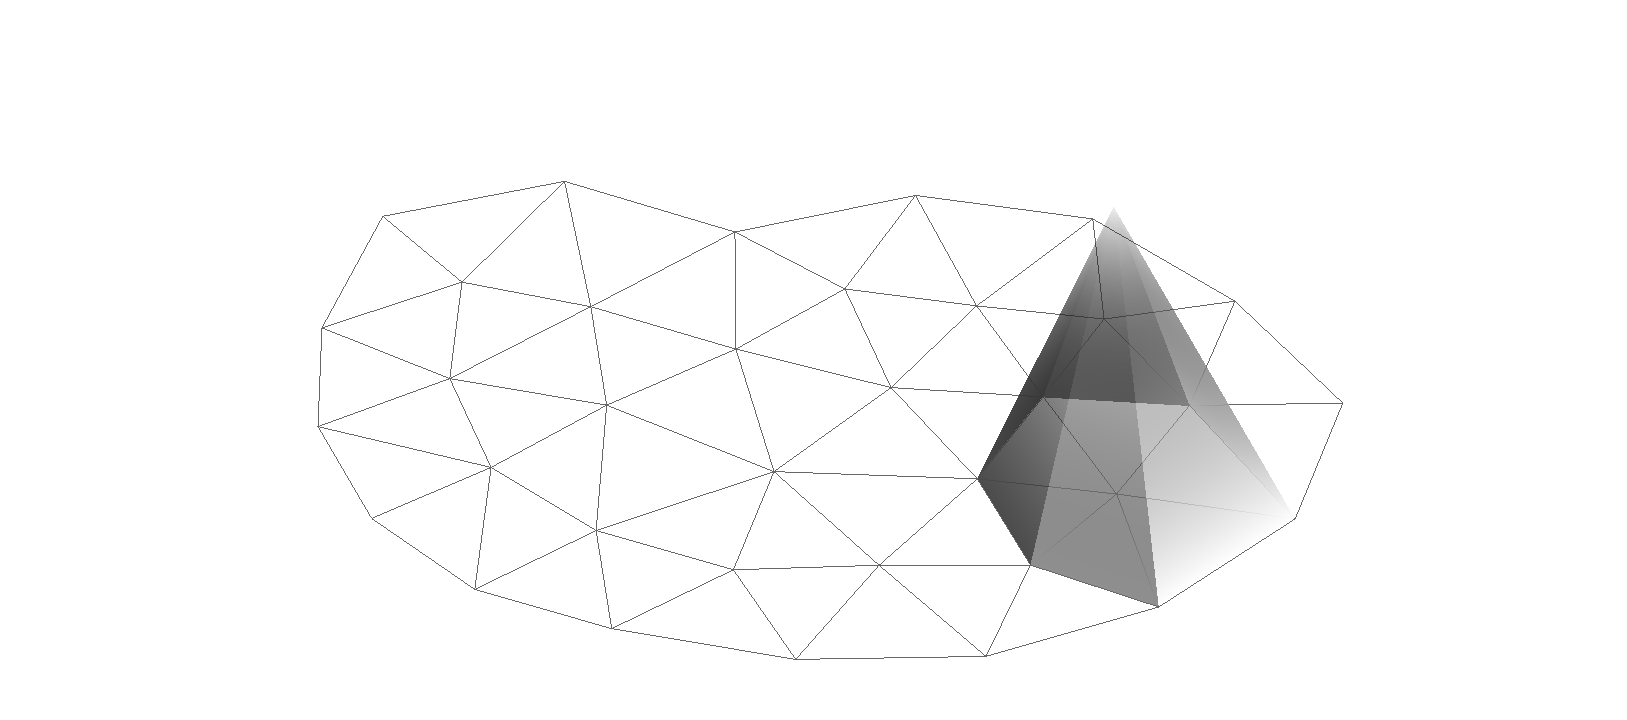
\includegraphics{040-discretizacion/shape-function-first-order-21.png}

}

}

\subcaption{\label{fig-shape-function-first-order-21}\(h_{21}(\vec{x})\)}
\end{minipage}%
%
\begin{minipage}[t]{0.05\linewidth}

{\centering 

~

}

\end{minipage}%
%
\begin{minipage}[t]{0.47\linewidth}

{\centering 

\raisebox{-\height}{

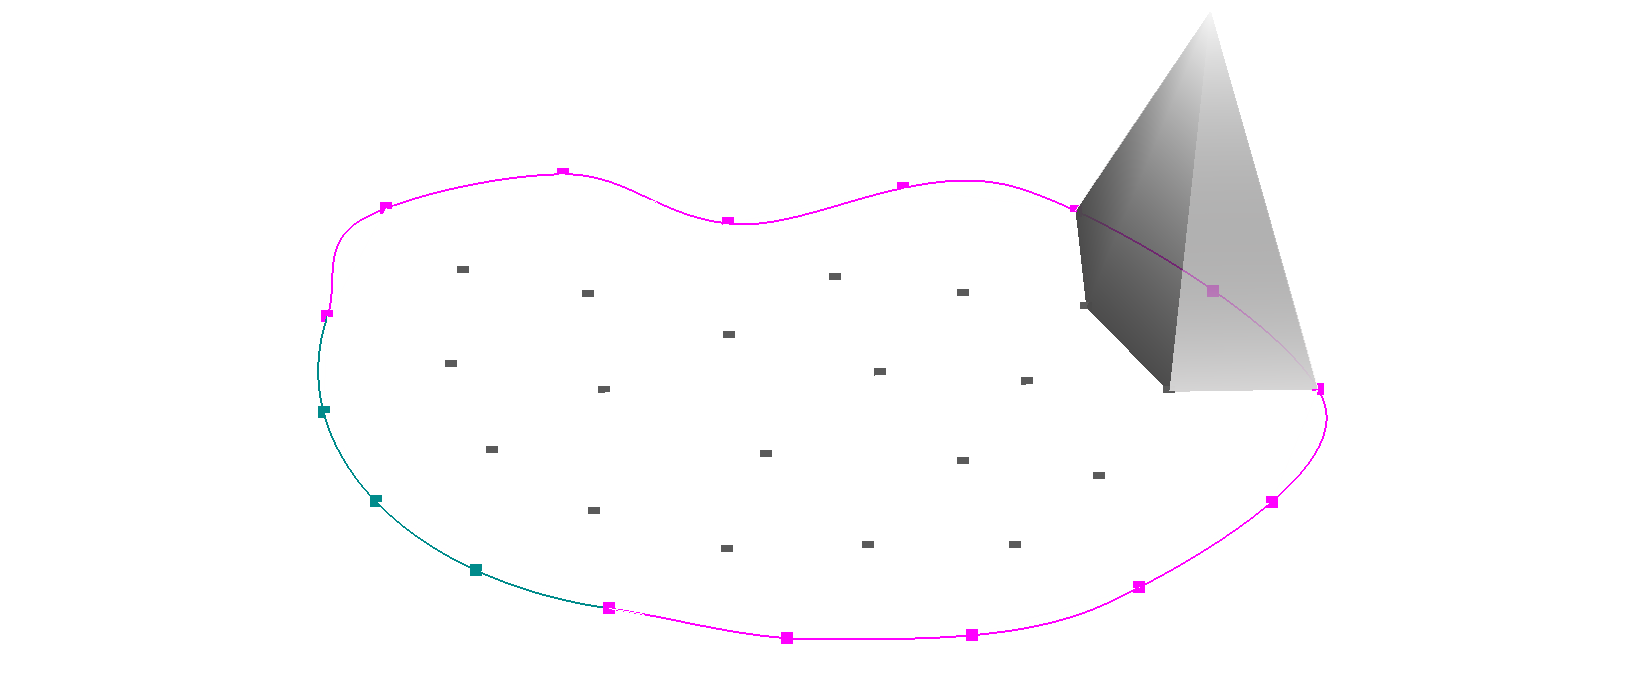
\includegraphics{040-discretizacion/shape-function-first-order-8.png}

}

}

\subcaption{\label{fig-shape-function-first-order-8}\(h_8(\vec{x})\)}
\end{minipage}%

\caption{\label{fig-shape-function-first-order}Funciones de forma de
primer orden apropiadas para diferentes puntos de
la~figura~\ref{fig-dominio-solo-nodos}. Una de las preguntas centrales
que el método de elementos finitos responde es ¿cómo encontrarlas?}

\end{figure}

Justamente, el método de elementos finitos propone una forma sistemática
para atacar estos dos puntos a partir de explotar la topología de
los~\(J\) puntos~\(\vec{x}_j\) de
la~figura~\ref{fig-dominio-solo-nodos}. El hecho de no haber incluido
puntos sobre la frontera~\(\Gamma_D\) en el conjunto de~\(J\) funciones
de forma de alguna manera rompe el sistematismo necesario para aplicar
el método. Lo primero que tenemos que hacer entonces es incluir puntos
sobre la frontera~\(\Gamma_D\). Digamos que hay~\(J_D\) puntos
sobre~\(\Gamma_D\). Entonces agregamos~\(J_D\) funciones de forma
para~\(j=J+1,\dots,J+J_D\) a las cuales les pedimos que

\[
h_j(\vec{x}_i) = \delta_{ji} \quad \text{para \quad $j=J+1,\dots,J+J_D$ \quad e \quad $i=1,\dots,J+J_D$}\\
\]

Es decir, que estas nuevas funciones de forma se anulen en los
demás~\(J+J_D-1\) puntos pero no necesitamos que se anulen en la
frontera como le pedíamos a las primeras funciones de forma
``originales'' para \(j \leq J\). Como las funciones de forma originales
cumplen las condiciones de la~ecuación~\ref{eq-forma-delta-0}, es decir
sí se anulan en

\begin{enumerate}
\def\labelenumi{\alph{enumi}.}
\tightlist
\item
  todos los nodos diferentes de~\(j\), y
\item
  en todos los puntos~\(\vec{x} \in \Gamma_D\)
\end{enumerate}

entonces también cumplen

\[
h_j(\vec{x}_i) = \delta_{ji} \quad \text{para \quad $j=1,\dots,J$ \quad e \quad $i=1,\dots,J+J_D$}\\
\]

Luego

\[
h_j(\vec{x}_i) = \delta_{ji} \quad \text{para \quad $j=1,\dots,J+J_D$ \quad e \quad $i=1,\dots,J+J_D$}\\
\] y recuperamos una parte la sistematicidad requerida para aplicar el
método de elementos finitos. Para recuperar la otra parte re-escribimos
la~ecuación~\ref{eq-v-vjhj} poniendo coeficientes iguales a cero en las
funciones de forma sobre~\(\Gamma_D\)

\[
v(\vec{x}) = \sum_{j=1}^J v_j \cdot h_j(\vec{x}) =
\sum_{j=1}^J v_j \cdot h_j(\vec{x}) + \sum_{j=J+1}^{J+J_D} 0 \cdot h_j(\vec{x})
\] que, en forma matricial, queda

\[
v(\vec{x}) = \tilde{\mat{H}}(\vec{x}) \cdot \tilde{\vec{v}} = \tilde{\vec{v}}^T \cdot \tilde{\mat{H}}^T(\vec{x})
\] donde ahora los objetos tildados son objetos ``extendidos''
incluyendo los~\(J_D\) puntos sobre~\(\Gamma_D\) como

\begin{equation}\protect\hypertarget{eq-H-ext}{}{
\tilde{\mat{H}}(\vec{x}) =
\begin{bmatrix}
h_1(\vec{x}) & h_2(\vec{x}) & \cdots & h_j(\vec{x}) & \cdots & h_J(\vec{x}) & h_{J+1}(\vec{x}) & \cdots & h_{J+J_D}(\vec{x})
\end{bmatrix}
}\label{eq-H-ext}\end{equation} y \[
\tilde{\vec{v}} = 
\begin{bmatrix}
v_1 \\
v_2 \\
\vdots \\
v_j \\
\vdots \\
v_J \\
0 \\
\vdots \\
0
\end{bmatrix}
\]

De la misma manera extendemos la matriz~\(\mat{B}(\vec{x})\) como

\begin{equation}\protect\hypertarget{eq-B-ext}{}{
\tilde{\mat{B}}(\vec{x}) =
\begin{bmatrix}
\displaystyle \frac{\partial h_1}{\partial x} & \displaystyle \frac{\partial h_2}{\partial x} & \cdots & \displaystyle \frac{\partial h_j}{\partial x} & \cdots & \displaystyle \frac{\partial h_J}{\partial x} & \displaystyle \frac{\partial h_{J+1}}{\partial x} & \cdots & \displaystyle \frac{\partial h_{J+J_D}}{\partial x} \\
\displaystyle \frac{\partial h_1}{\partial y} & \displaystyle \frac{\partial h_2}{\partial y} & \cdots & \displaystyle \frac{\partial h_j}{\partial y} & \cdots & \displaystyle \frac{\partial h_J}{\partial y} & \displaystyle \frac{\partial h_{J+1}}{\partial y} & \cdots & \displaystyle \frac{\partial h_{J+J_D}}{\partial y} \\
\displaystyle \frac{\partial h_1}{\partial z} & \displaystyle \frac{\partial h_2}{\partial z} & \cdots & \displaystyle \frac{\partial h_j}{\partial z} & \cdots & \displaystyle \frac{\partial h_J}{\partial z} & \displaystyle \frac{\partial h_{J+1}}{\partial z} & \cdots & \displaystyle \frac{\partial h_{J+J_D}}{\partial z} \\
\end{bmatrix}
}\label{eq-B-ext}\end{equation}

Repitiendo todos los pasos, el método de Galerkin requiere que

\begin{equation}\protect\hypertarget{eq-extendida}{}{
\tilde{\vec{v}}^T \cdot \left[ \int_U \tilde{\mat{B}}^T(\vec{x}) \cdot k(\vec{x}) \cdot \tilde{\mat{B}}(\vec{x}) \, d^D\vec{x} \right] \cdot \tilde{\vec{u}}
=
\tilde{\vec{v}}^T \cdot \left[ \int_{U} \tilde{\mat{H}}^T(\vec{x}) \cdot f(\vec{x}) \, d^D \vec{x}
+ \int_{\Gamma_N} \tilde{\mat{H}}^T(\vec{x}) \cdot p(\vec{x}) \, d^{D-1}\vec{x} \right]
}\label{eq-extendida}\end{equation} para
todo~\(\tilde{v}^T = \begin{bmatrix} v_1 & \cdots \ v_J & 0 & \cdots & 0\end{bmatrix}\).

\begin{theorem}[]\protect\hypertarget{thm-extendida}{}\label{thm-extendida}

Este requerimiento es equivalente a~\(\mat{A} \cdot \vec{u} = \vec{b}\).

\begin{proof}

Sean los objetos extendidos

\[
\tilde{\vec{v}} =
\begin{bmatrix}
\vec{v} \\
\vec{0}
\end{bmatrix}
\quad
\tilde{\mat{A}} =
\begin{bmatrix}
\mat{A} & \mat{C} \\
\mat{D} & \mat{E} \\
\end{bmatrix}
\quad
\tilde{\vec{u}} =
\begin{bmatrix}
\vec{u} \\
\vec{0}
\end{bmatrix}
\quad
\tilde{\vec{b}} =
\begin{bmatrix}
\vec{b} \\
\vec{e}
\end{bmatrix}
\]

Entonces

\[
\begin{aligned}
\tilde{\vec{v}}^T \cdot \tilde{\mat{A}} \cdot \tilde{\vec{u}}
&=
\tilde{\vec{v}}^T \cdot \tilde{\vec{b}} \\
\begin{bmatrix} \vec{v}^T & \vec{0}^T \end{bmatrix}
\cdot
\begin{bmatrix}
\mat{A} & \mat{C} \\
\mat{D} & \mat{E} \\
\end{bmatrix}
\cdot
\begin{bmatrix}
\vec{u} \\
\vec{0}
\end{bmatrix}
& =
\begin{bmatrix} \vec{v}^T & \vec{0}^T \end{bmatrix}
\begin{bmatrix}
\vec{b} \\
\vec{e}
\end{bmatrix}
\\
\begin{bmatrix} \vec{v}^T & \vec{0}^T \end{bmatrix}
\cdot
\begin{bmatrix}
\mat{A} \cdot \vec{u} + \mat{C} \cdot \vec{0} \\
\mat{D} \cdot \vec{u} + \mat{E} \cdot \vec{0} \\
\end{bmatrix}
&=
\begin{bmatrix} \vec{v}^T & \vec{0}^T \end{bmatrix}
\begin{bmatrix}
\vec{b} \\
\vec{e}
\end{bmatrix}
\\
\vec{v}^T \cdot \mat{A} \cdot \vec{u} + \vec{0}^T \cdot \mat{D} \cdot \vec{u}
&=
\vec{v}^T \cdot \vec{b} + \vec{0}^T \cdot \vec{e}\\
\vec{v}^T \cdot \mat{A} \cdot \vec{u}
&=
\vec{v}^T \cdot \vec{b}\\
\end{aligned}
\]

Como esta igualdad debe valer~\(\forall \vec{v}\),
entonces~\(\mat{A} \cdot \vec{u} - \vec{b} = 0\).

\end{proof}

\end{theorem}

\begin{corollary}[]\protect\hypertarget{cor-irrelevancia}{}\label{cor-irrelevancia}

Si~\(\tilde{\vec{v}}=\begin{bmatrix} \vec{v} & \vec{0}\end{bmatrix}^T\)
y~\(\tilde{\vec{u}}=\begin{bmatrix} \vec{u} & \vec{0}\end{bmatrix}^T\)
entonces el contenido de las matrices~\(\mat{C}\), \(\mat{D}\)
y~\(\mat{E}\) y del vector~\(\vec{e}\) es irrelevante.

\end{corollary}

\begin{theorem}[]\protect\hypertarget{thm-A-monio-es-singular}{}\label{thm-A-monio-es-singular}

La matriz~\(\tilde{\mat{A}}\) es singular. Más aún,
\(\ker{(\tilde{\mat{A}})} = 1\).

\textbf{TODO}

\end{theorem}

\begin{corollary}[]\protect\hypertarget{cor-K-phi}{}\label{cor-K-phi}

Sean los objetos

\begin{equation}\protect\hypertarget{eq-K}{}{
\mat{K} =
\begin{bmatrix}
\mat{A} & \mat{C} \\
\mat{0} & \mat{I} \\
\end{bmatrix}
\quad
\vec{f} =
\begin{bmatrix}
\vec{b} \\
\vec{0} \\
\end{bmatrix}
}\label{eq-K}\end{equation} tales
que~\(\mat{A} \cdot \vec{u} = \vec{b}\), donde~\(\mat{I}\) es la matriz
identidad de tamaño~\(J_D \times J_D\). Entonces el
vector~\(\symbf{\varphi}\) tal que
\(\mat{K} \cdot \symbf{\varphi} = \vec{f}\) es igual a

\[
\symbf{\varphi}
 =
\begin{bmatrix}
\vec{u} \\
\vec{0} \\
\end{bmatrix}
\]

\begin{proof}

Sea~\(\symbf{\varphi} = \begin{bmatrix} \symbf{\varphi}_1 & \symbf{\varphi}_2 \end{bmatrix}^T\).
Entonces \(\mat{K} \cdot \symbf{\varphi}\) es

\[
\begin{bmatrix}
\mat{A} & \mat{C} \\
\mat{0} & \mat{I}
\end{bmatrix}
\cdot
\begin{bmatrix}
\symbf{\varphi}_1 \\
\symbf{\varphi}_2 
\end{bmatrix}
=
\begin{bmatrix}
\mat{A} \cdot \symbf{\varphi}_1 + \mat{C} \cdot \symbf{\varphi}_2\\
\mat{0} \cdot \symbf{\varphi}_1 + \mat{I} \cdot \symbf{\varphi}_2
\end{bmatrix}
=
\begin{bmatrix}
\vec{b}\\
\vec{0}
\end{bmatrix}
\]

De la segunda fila se tiene~\(\symbf{\varphi}_2 = \vec{0}\).
Reemplazando este resultado en la primera fila,
\(\mat{A} \cdot \symbf{\varphi}_1 = \vec{b}\).
Luego~\(\symbf{\varphi}_1 = \mat{A}^{-1} \cdot \vec{b} = \vec{u}\).

\end{proof}

\end{corollary}

La importancia de este resultado radica en que si pudiésemos construir
la matriz
extendida~\(\tilde{\mat{A}} \in \mathbb{R}^{(J+J_D)\times(J+J_D)}\)
donde el elemento de la fila~\(i\) y la columna~\(j\) es

\[
\tilde{a}_{ij} = \mathcal{a}\Big(h_i(\vec{x}), h_j(\vec{x})\Big)
\quad \text{para $i=1,\dots,J+J_D$ y $j=1,\dots,J+J_D$}
\] sin distinguir entre nodos en~\(U\), en~\(\Gamma_N\) o
en~\(\Gamma_D\), entonces podríamos obtener la matriz~\(\mat{K}\)
reemplazando las filas correspondientes a~\(i=J+1,\dots,J+J_D\) por
todos ceros, excepto un uno (o cualquier valor~\(\alpha \neq 0\)) en la
diagonal. Al mismo tiempo, tendríamos que reemplazar los elementos del
vector~\(\vec{f}\)

\[
f_j = \mathcal{B}\Big(h_j(\vec{x})\Big)
\quad \text{para $J=1,\dots,J+J_D$}
\] para~\(j > J\) por \(f_j=0\).

\begin{definition}[matriz de
rigidez]\protect\hypertarget{def-rigidez}{}\label{def-rigidez}

La matriz cuadrada~\(\mat{K}\) de tamaño igual a la cantidad
total~\(J+J_D\) de nodos tal que
\(\mat{K} \cdot \symbf{\varphi} = \vec{f}\) se llama (usualmente)
\emph{matriz de rigidez}.

\end{definition}

\begin{theorem}[]\protect\hypertarget{thm-K-no-singular}{}\label{thm-K-no-singular}

La matriz de rigidez tiene inversa.

\begin{proof}

La matriz~\(\mat{K}\) tiene una estructura de bloque triangular superior

\[
\mat{K} =
\begin{bmatrix}
\mat{A} & \mat{C} \\
\mat{0} & \mat{I} \\
\end{bmatrix}
\]

Luego su determinante es

\[
\det{(\mat{K})} = \det{(\mat{A})} \cdot \det{(\mat{I})} = \det{(\mat{A})} \neq 0
\] ya que~\(\mat{A}\) es definida positiva por
el~teorema~\ref{thm-A-spd}.

\end{proof}

\end{theorem}

\begin{remark}

Aún cuando la matriz~\(\mat{A}\) sea simétrica, la matriz de
rigidez~\(\mat{K}\) (ecuación~\ref{eq-K}) no lo es. Sin embargo, es
posible realizar el procedimiento de reemplazar filas por ceros excepto
en la diagonal agregando operaciones extra de reemplazo de columans por
ceros excepto en la diagonal mientras al mismo tiempo se realizan
operaciones equivalentes sobre el vector~\(\vec{f}\) del miembro derecho
de forma tal de obtener un sistema de ecuaciones equivalente donde la
matriz sea simétrica. Estos detalles forman parte de la implementación
computacional y no de la teoría detrás del método numérico.

\end{remark}

\begin{remark}

El procedimiento propuesto para obtener la matriz de rigidez no es el
único. Otra formas de incorporar las condiciones de Dirichlet a la
matriz de rigidez incluyen {[}12{]}

\begin{enumerate}
\def\labelenumi{\arabic{enumi}.}
\tightlist
\item
  Eliminación directa
\item
  Método de penalidad
\item
  Multiplicadores de Lagrange
\end{enumerate}

De todas maneras, este procedimiento\ldots{}

\begin{enumerate}
\def\labelenumi{\alph{enumi}.}
\tightlist
\item
  es computacionalmente eficiente (especialmente si se elige la
  constante~\(\alpha \neq 0\) que se pone en la diagonal de las filas de
  Dirichlet en forma apropiada y se mantiene la simetría de la matriz
  del sistema de ecuaciones), y
\item
  permite incorporar condiciones de contorno de Dirichlet no homogéneas
  de una forma muy natural como mostramos a continuación.
\end{enumerate}

\end{remark}

En efecto, supongamos ahora que tengamos que resolver el problema de
la~ecuación~\ref{eq-no-homogeneo} con una condición de contorno de
Dirichlet no homogénea

\[
u(\vec{x}) = g(\vec{x}) \quad \forall \vec{x} \in \Gamma_D
\]

La forma de resolver el problema continuo que introdujimos en la
sección~\ref{sec-dirichlet-nh} fue considerar~\(u_g \in H_g^1\),
escribir~\(u_h = u - u_g\) y encontrar~\(u_h \in V\) tal que

\[
\mathcal{a}(u_h,v) = \mathcal{B}(v) - \mathcal{a}(u_g,v) \quad \forall v \in V
\]

Ahora,

\begin{enumerate}
\def\labelenumi{\arabic{enumi}.}
\item
  volvemos a pasar~\(\mathcal{a}(u_g,v)\) al miembro izquierdo
  aprovechando la bilinealidad de~\(a\)

  \[
  \mathcal{a}(u_h+u_g,v) = \mathcal{a}(u,v) = \mathcal{B}(v)
  \]
\item
  escribimos la parte homogénea~\(u_h\) como

  \[
  u_h(\vec{x}) = \sum_{j=1}^{J} h_j(\vec{x}) \cdot u_j + \sum_{j=J+1}^{J+J_D} h_j(\vec{x}) \cdot 0
  = \tilde{\mat{H}} \cdot \begin{bmatrix} \vec{u} \\ \vec{0} \end{bmatrix}
  \]
\item
  la función auxiliar~\(u_g\) que satisface la condición de Dirichlet
  como

  \[
  u_g(\vec{x}) = \sum_{j=1}^{J} h_j(\vec{x}) \cdot 0 + \sum_{j=J+1}^{J+J_D} h_j(\vec{x}) \cdot g(\vec{x}_j)
  = \tilde{\mat{H}} \cdot \begin{bmatrix} \vec{0} \\ \vec{g} \end{bmatrix}
  \]
\item
  y la suma~\(u=u_h+u_g\)

  \[
  u(\vec{x}) = u_h(\vec{x}) + u_g(\vec{x}) = \sum_{j=1}^{J} h_j(\vec{x}) \cdot u_j + \sum_{j=J+1}^{J+J_D} h_j(\vec{x}) \cdot g(\vec{x}_j)
  = \tilde{\mat{H}} \cdot \tilde{\vec{u}}
  \] donde ahora extendemos~\(\vec{u}\) como

  \[
  \tilde{\vec{u}} =
  \begin{bmatrix}
  \vec{u} \\
  \vec{g}
  \end{bmatrix}
  \] y

  \[
  \vec{g} =
  \begin{bmatrix}
  g(\vec{x}_{J+1}) \\
  g(\vec{x}_{J+2}) \\
  \vdots \\
  g(\vec{x}_{J+J_D}) \\
  \end{bmatrix}
  \]
\end{enumerate}

Como~\(v(\vec{x}) \in V_J \subset H^1_0\), entonces~\(\vec{v}\) todavía
se extiende con ceros

\[
\tilde{\vec{v}} =
\begin{bmatrix}
\vec{v} \\
\vec{0}
\end{bmatrix}
\] y el problema discretizado queda

\[
\begin{aligned}
\begin{bmatrix}
\vec{v}^T & \vec{0}^T
\end{bmatrix}
\cdot
\begin{bmatrix}
\mat{A} & \mat{C} \\
\mat{D} & \mat{E}
\end{bmatrix}
\cdot
\begin{bmatrix}
\vec{u} \\
\vec{g}
\end{bmatrix}
&=
\begin{bmatrix}
\vec{v}^T & \vec{0}^T
\end{bmatrix}
\cdot
\begin{bmatrix}
\vec{b} & \vec{e}
\end{bmatrix} \\
\begin{bmatrix}
\vec{v}^T & \vec{0}^T
\end{bmatrix}
\cdot
\begin{bmatrix}
\mat{A} \cdot \vec{u} + \mat{C} \cdot \vec{g} \\
\mat{D} \cdot \vec{u} + \mat{E} \cdot \vec{g}
\end{bmatrix}
&=
\begin{bmatrix}
\vec{v}^T & \vec{0}^T
\end{bmatrix}
\cdot
\begin{bmatrix}
\vec{b} & \vec{e}
\end{bmatrix} \\
\vec{v}^T \cdot \mat{A} \cdot \vec{u} + \vec{v}^T \cdot \mat{C} \cdot \vec{g} &= \vec{v}^T \cdot \vec{b}
\end{aligned}
\] para todo~\(\vec{u} \in \mathbb{R}^J\). Es decir, la aproximación de
Galerkin para el problema con condiciones de Dirichlet no homogéneas es

\begin{equation}\protect\hypertarget{eq-discretizado-nh}{}{
\mat{A} \cdot \vec{u} + \mat{C} \cdot \vec{g} = \vec{b}
}\label{eq-discretizado-nh}\end{equation}

\begin{corollary}[]\protect\hypertarget{cor-K-phi-nh}{}\label{cor-K-phi-nh}

Sean los objetos

\[
\mat{K} =
\begin{bmatrix}
\mat{A} & \mat{C} \\
\mat{0} & \mat{I} \\
\end{bmatrix}
\quad
\vec{f} =
\begin{bmatrix}
\vec{b} \\
\vec{g} \\
\end{bmatrix}
\] tales que se satisface la~ecuación~\ref{eq-discretizado-nh}, entonces
el vector~\(\symbf{\varphi}\) tal que
\(\mat{K} \cdot \symbf{\varphi} = \vec{f}\) es igual a

\[
\symbf{\varphi}
 =
\begin{bmatrix}
\vec{u} \\
\vec{g} \\
\end{bmatrix}
\]

\begin{proof}

Sea~\(\symbf{\varphi} = \begin{bmatrix} \symbf{\varphi}_1 & \symbf{\varphi}_2 \end{bmatrix}^T\).
Entonces \(\mat{K} \cdot \symbf{\varphi}\) es

\[
\begin{bmatrix}
\mat{A} & \mat{C} \\
\mat{0} & \mat{I}
\end{bmatrix}
\cdot
\begin{bmatrix}
\symbf{\varphi}_1 \\
\symbf{\varphi}_2 
\end{bmatrix}
=
\begin{bmatrix}
\mat{A} \cdot \symbf{\varphi}_1 + \mat{C} \cdot \symbf{\varphi}_2\\
\mat{0} \cdot \symbf{\varphi}_1 + \mat{I} \cdot \symbf{\varphi}_2
\end{bmatrix}
=
\begin{bmatrix}
\vec{b}\\
\vec{g}
\end{bmatrix}
\]

De la segunda fila se tiene~\(\symbf{\varphi}_2 = \vec{g}\).
Reemplazando este resultado en la primera fila,

\[
\mat{A} \cdot \symbf{\varphi}_1 + \mat{C} \cdot \vec{g} = \vec{b}
\]

Dado que se satisface la~ecuación~\ref{eq-discretizado-nh}
entonces~\(\symbf{\varphi}_1 = \vec{u}\).

\end{proof}

\end{corollary}

\begin{remark}

Los corolarios~\ref{cor-K-phi} y~\ref{cor-K-phi-nh} muestran que el
procedimiento de reemplazar las filas correspondientes a los puntos
de~\(\Gamma_D\) por ceros excepto un uno (o~\(\alpha \neq 0\)) en la
diagonal y por el valor de la condición de contorno~\(g(\vec{x}_j)\)
(o~\(\alpha \cdot g(\vec{x}_j)\)) en dicho punto funciona tanto para
condiciones homogéneas como no homogéneas.

\end{remark}

\begin{remark}

Para el caso no homogéneo, el contenido de la matriz~\(\mat{C}\) que
contiene el resultado de aplicar el operador~\(\mathcal{a}\) entre las
funciones de forma del interior de~\(U\) y de~\(\Gamma_N\) contra las
funciones de forma de~\(\Gamma_D\)

\[
c_{i,j-J} = \mathcal{a}\left(h_i(\vec{x}),h_j(\vec{x})\right) \quad \text{para $i=1,\dots,J$ y $j=J+1,J+J_D$}
\]

no es irrelevante como lo era para el caso~\(g(\vec{x})=0\).

\end{remark}

Estamos entonces en condiciones resolver el primero de los dos puntos
de la página~\pageref{dos}: ¿cómo encontramos \(J+J_D\) funciones de
forma apropiadas? Para ello, consideramos la topología subyacente en los
\(J+J_D\) puntos. Tomemos la~figura~\ref{fig-dominio-nodos-elementos},
que muestra no sólo los~\(J_D\) puntos sobre~\(\Gamma_D\) sino los
triángulos que forman los~\(J+J_D\) puntos.

\begin{figure}

{\centering 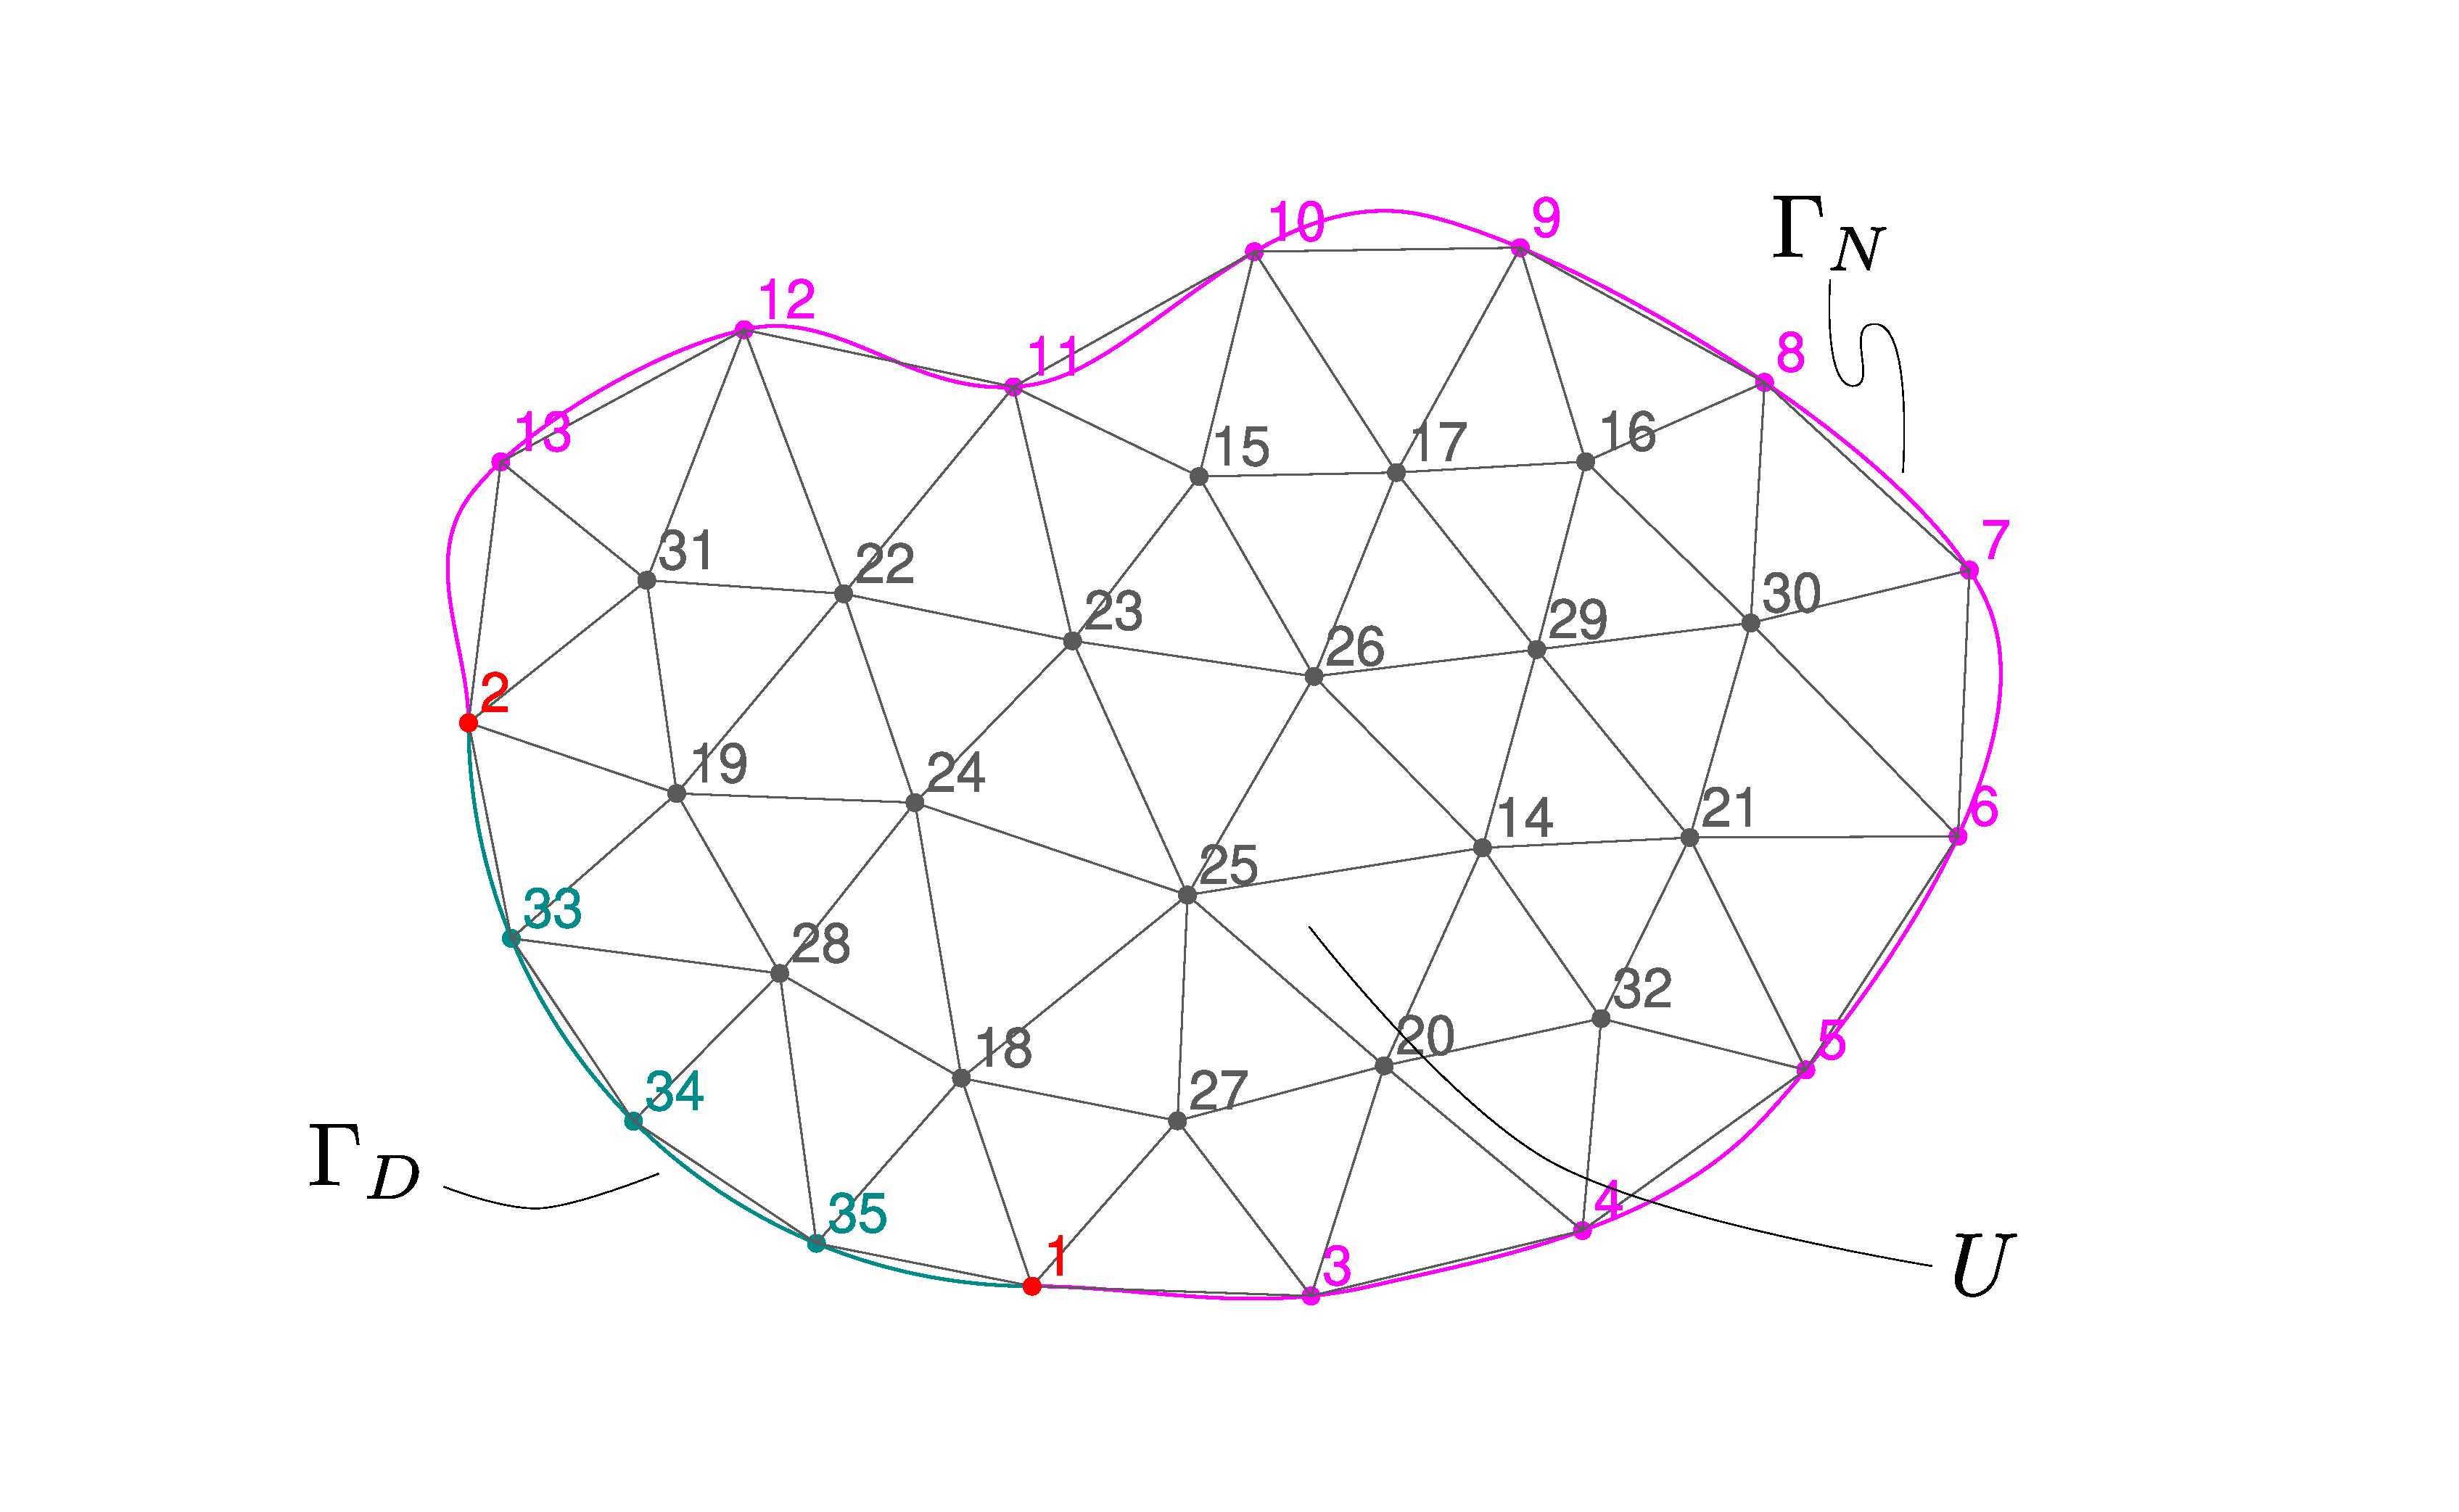
\includegraphics[width=0.75\textwidth,height=\textheight]{040-discretizacion/dominio-nodos-elementos.pdf}

}

\caption{\label{fig-dominio-nodos-elementos}El dominio espacial~\(U\) de
la figura~\ref{fig-dominio-solo-nodos} con \(J_D=3\) puntos extra en la
frontera~\(\Gamma_D\) para~ \(j=33,34,35\). Además, se muestran los
triángulos que conectan los puntos entre sí y que cubren el
dominio~\(U\).}

\end{figure}

\begin{definition}[elemento]\protect\hypertarget{def-elemento}{}\label{def-elemento}

Un \emph{elemento} es una entidad topológica de dimensión~\(D=0,1,2\)
o~\(3\) capaz de cubrir un dominio espacial~\(U \in \mathbb{R}^D\).

\textbf{TODO}

\end{definition}

\begin{definition}[nodo]\protect\hypertarget{def-nodo}{}\label{def-nodo}

Llamamos a cada uno de los puntos que define un elemento, \emph{nodo}.

\end{definition}

\begin{definition}[valor
nodal]\protect\hypertarget{def-v_j}{}\label{def-v_j}

Dado que~\(h_j(\vec{x}_i) = \delta_{ji}\) entonces los
coeficientes~\(v_j\) son iguales a la función~\(v\) evaluada
en~\(\vec{x}_j\), es decir el valor que toma la función en el nodo~\(j\)

\[
v_j = v(\vec{x}_j)
\]

Llamamos a \(v_j\), el \emph{valor nodal} de la solución aproximada.

\end{definition}

\begin{remark}

Los~\(J\) valores nodales~\(u_j\) son las incógnitas que se obtienen al
resolver el problema numéricamente. Pero la solución al problema de
Galerkin no es simplemente un conjunto de coeficientes sino una función
continua~\(u_N(\vec{x})\) que puede ser evaluada en cualquier punto del
espacio~\(\vec{x} \in U\).

\end{remark}

\begin{corollary}[]\protect\hypertarget{cor-suma-a-no}{}\label{cor-suma-a-no}

Para que sea posible recuperar exactamente una función
constante~\(u(\vec{x})= \text{cte} \in U\) a partir de valores nodales
constantes~\(u_j = \text{cte}\) las funciones de forma deben sumar
uno~\(\forall \vec{x} \in U\). En resumen, las funciones de forma deben
cumplir

\begin{equation}\protect\hypertarget{eq-condiciones-h}{}{
\begin{cases}
h_j(\vec{x}_i) = \delta_{ij} &\quad \text{para \quad $j=1,\dots,J+J_D$ \quad e \quad $i=1,\dots,J+J_D$} \\
\displaystyle \sum_{j=1}^{J+J_D} h_j(\vec{x}) = 1  &\quad \forall \vec{x} \in U ~\text{(incluyendo la frontera $\partial U$)}
\end{cases}
}\label{eq-condiciones-h}\end{equation}

\end{corollary}

Si los elementos son apropiados, la integral sobre el dominio~\(U\) es
aproximadamente igual a la suma de las integrales sobre cada uno de
los~\(I\) elementos~\(e_1\), \(e_2\), \ldots, \(e_I\) en los que lo
dividimos. De hecho, los elementos son ``apropiados'' justamente si a
medida que dividimos el dominio en más y más elementos cada vez de menor
tamaño (lo que implica que~\(J \rightarrow \infty\)), entonces

\[
\lim_{I \rightarrow \infty} \sum_{i=1}^I \int_{e_i} f(\vec{x}) \, d^D\vec{x} = \int_{U} f(\vec{x}) \, d^D\vec{x}
\] para cualquier función~\(f(\vec{x}) : U \mapsto \mathbb{R}\)
integrable.

La idea básica del método de elementos finitos (al menos para problemas
lineales) es justamente concentrarse en escribir las integrales que
definen la matriz de rigidez y el vector del miembro derecho en cada uno
de los elementos~\(e_i\) para luego ``ensamblar'' estos objetos globales
a partir de las contribuciones elementales. Justamente, este proceso de
enfocarse en los elementos es muy eficiente desde del punto de vista
computacional ya que se presta perfectamente para ser realizado en forma
paralela como mostramos en el~\textbf{?@sec-implementacion}.

Para fijar ideas, supongamos por un momento que tenemos un elemento
triangular en el plano~\(x\)-\(y\) cuyos vértices son

\[
\begin{aligned}
\vec{x}_1 &= \begin{bmatrix}0 & 0\end{bmatrix} \\
\vec{x}_2 &= \begin{bmatrix}1 & 0\end{bmatrix} \\
\vec{x}_3 &= \begin{bmatrix}0 & 1\end{bmatrix} \\
\end{aligned}
\]

\textbf{TODO} figura (desde FeenoX/Gmsh)

Consideremos las funciones

\[
\begin{aligned}
h_1(\vec{x}) &= 1 - x - y \\
h_2(\vec{x}) &= x \\
h_3(\vec{x}) &= y \\
\end{aligned}
\]

Si el triángulo fuese el dominio~\(U \mathbb{R}^2\) y quisiéramos
resolver una ecuación diferencial en derivadas parciales discretizándolo
con los tres nodos~\(\vec{x}_1\), \(\vec{x}_2\) y~\(\vec{x}_3\) entonces
estas funciones de forma cumplirían los requerimientos de
la~ecuación~\ref{eq-condiciones-h}. Recordando las
ecuaciones~\ref{eq-H-ext} y~\ref{eq-B-ext}, para un problema escalar el
número grados de libertad por nodo es~\(G=1\)

\[
\begin{aligned}
\tilde{\mat{H}}(\vec{x}) &= \begin{bmatrix} 1-x-y & x & y \end{bmatrix}  \quad \mathbb{R}^{G \times J}\\
\tilde{\mat{B}}(\vec{x}) &= \begin{bmatrix} -1 & +1 & 0 \\ -1 & 0 & +1\end{bmatrix} \quad \mathbb{R}^{D \times J}
\end{aligned}
\]

Usando las expresiones de la~ecuación~\ref{eq-A-b-poisson}, podemos
calcular explícitamente la matriz aumentada~\(\tilde{\mat{A}}\) como

\[
\tilde{\mat{A}} = \bigintss_e
\begin{bmatrix}
-1 & -1 \\
+1 & 0 \\
0 & +1 \\
\end{bmatrix}
 \cdot k(\vec{x}) \cdot 
\begin{bmatrix} -1 & +1 & 0 \\ -1 & 0 & +1 \end{bmatrix}
\, d^D\vec{x} \\
=
\begin{bmatrix}
   2  & -1  & -1  \\
  -1  &  1  &  0  \\
  -1  &  0  &  1  \\
\end{bmatrix}
\cdot
\int_e f(\vec{x}) \, d^D\vec{x}
\] donde~\(e\) se refiere al elemento triangular. Si~\(f(\vec{x})=1\),
entonces la integral es el área del triángulo que es \(1/2\). Lo
importante del ejemplo es que la matriz de rigidez elemental

\begin{enumerate}
\def\labelenumi{\arabic{enumi}.}
\tightlist
\item
  es cuadrada de tamaño~\(GJ \times GJ\) siendo~\(G=1\) para un problema
  escalar como la ecuación de Poisson y~\(J\) es el número de nodos del
  elemento
\item
  conocidas las funciones de forma del elemento, se puede calcular
  fácilmente primero derivando las~\(h_j\) con respecto a las variables
  espaciales y luego integrando la misma expresión de la matriz
  extendida global sobre el elemento.
\end{enumerate}

En este caso en particular, dado que las funciones de forma son lineales
con respecto a las variables espaciales entonces la
matriz~\(\mat{B}(\vec{x})\) es uniforme y puede salir fuera de la
integral. Para otras topologías de elementos (por ejemplo cuadrángulos)
o para elementos de órdenes superiores (en los que se agregan nodos
sobre los lados o sobre el seno del elemento), las funciones de forma
tendrán una dependencia más compleja y sus derivadas dependerán
de~\(\vec{x}\) por lo que efectivamente habrá que integrar el
producto~\(\mat{B}^T(\vec{x}) k(\vec{x}) \mat{B}(\vec{x})\) sobre el
triángulo. Si bien en general es posible utilizar cualquier método de
cuadratura numérica (incluyendo métodos adaptivos), la forma usual de
calcular estas integrales es utilizando el método de integración de
Gauss que consiste en disponer de una cantidad pre-fijada~\(Q\) de pares
de pesos~\(\omega_q\) y puntos espaciales~\(\vec{x}_q\) tales que

\[
\int_e \vec{F}(\vec{x}) \, d^D \vec{x} \approx \sum_{q=1}^Q \omega_q \cdot \vec{F}(\vec{x}_q)
\] donde el número~\(Q\) depende de la precisión de la aproximación:
mientras mayor sea~\(Q\), mayor será la precisión de la integral (y
mayor será el costo computacional para calcularla).

Está claro que los elementos triangulares de
la~figura~\ref{fig-dominio-solo-nodos} no coinciden con el triángulo
canónico de vértices~\([0,0]\), \([1,0]\) y~\([0,1]\). Pero podemos
suponer que este elemento canónico~\(e_c\), cuya matriz elemental ya
sabemos calcular, vive en un plano bidimensional~\(\xi\)-\(\eta\). Si
pudiésemos encontrar, para cada elemento~\(e_i\) del dominio, una
transformación biyectiva entre las coordenadas reales~\(x\)-\(y\) y las
coordenadas canónicas~\(\xi\)-\(\eta\) entonces podríamos calcular por
un lado las integrales utilizando el jacobiano~\(\mat{J}\) de la
transformación~\(\vec{x} \mapsto \symbf{\xi}\)

\[
\int_{e_i} f(\vec{x}) \, d^2\vec{x} = \int_{e_c} f(\symbf{\xi}) \cdot \Big| \det{(\mat{J})} \Big| \, d^2\symbf{\xi}
\] y por otro las derivadas con respecto a las coordenadas
originales~\(x\)-\(y\) que aparezcan en los integrandos utilizando la
regla de la cadena

\[
\begin{aligned}
\frac{\partial f}{\partial x} &= \frac{\partial f}{\partial \xi} \cdot \frac{\partial \xi}{\partial x} + \frac{\partial f}{\partial \eta} \cdot \frac{\partial \eta}{\partial x} \\
\frac{\partial f}{\partial y} &= \frac{\partial f}{\partial \xi} \cdot \frac{\partial \xi}{\partial y} + \frac{\partial f}{\partial \eta} \cdot \frac{\partial \eta}{\partial y} \\
\end{aligned}
\]

Para ello consideremos la siguiente transformación inversa
de~\(\symbf{\xi}\) a \(\vec{x}\)

\[
\begin{aligned}
x &= h_1(\symbf{\xi}) \cdot x_1 + h_2(\symbf{\xi}) \cdot x_2 + h_3(\symbf{\xi}) \cdot x_3 = \sum_{j=1}^3 h_j(\symbf{\xi}) \cdot x_j \\
y &= h_1(\symbf{\xi}) \cdot y_1 + h_2(\symbf{\xi}) \cdot y_2 + h_3(\symbf{\xi}) \cdot y_3 = \sum_{j=1}^3 h_j(\symbf{\xi}) \cdot y_j \\
\end{aligned}
\] donde~\(x_j\) e~\(y_j\) son las coordenadas del nodo~\(j\)-ésimo del
elemento (triángulo) \(e_i\). Es decir, la transformación (inversa)
propuesta consiste en interpolar las coordenadas reales
continuas~\(\vec{x}\) a partir de las coordenadas reales~\(\vec{x}_j\)
de los nodos del elemento real~\(e_i\) usando las funciones de forma del
elemento canónico~\(e_c\).\footnote{Explicar isoparamétrico
  \textbf{TODO}} Las derivadas parciales de~\(x\) e \(y\) con respecto
a~\(\xi\) y~\(\eta\) son

\begin{equation}\protect\hypertarget{eq-dxdxi}{}{
\begin{aligned}
\frac{\partial x}{\partial \xi}  &= \sum_{j=1}^3 \frac{\partial h_j}{\partial \xi}  \cdot x_j \\
\frac{\partial x}{\partial \eta} &= \sum_{j=1}^3 \frac{\partial h_j}{\partial \eta} \cdot x_j \\
\frac{\partial y}{\partial \xi}  &= \sum_{j=1}^3 \frac{\partial h_j}{\partial \xi}  \cdot y_j \\
\frac{\partial y}{\partial \eta} &= \sum_{j=1}^3 \frac{\partial h_j}{\partial \eta} \cdot y_j \\
\end{aligned}
}\label{eq-dxdxi}\end{equation}

Los diferenciales~\(dx\) y~\(dy\) se relacionan con los
diferenciales~\(d\xi\) y~\(d\eta\) como

\[
\begin{aligned}
dx &= \frac{\partial x}{\partial \xi} \cdot d\xi + \frac{\partial x}{\partial \eta} \cdot d\eta \\
dy &= \frac{\partial y}{\partial \xi} \cdot d\xi + \frac{\partial y}{\partial \eta} \cdot d\eta \\
\end{aligned}
\] que en forma matricial podemos escribir como

\begin{equation}\protect\hypertarget{eq-dxdy}{}{
\begin{bmatrix}
dx \\
dy
\end{bmatrix}
=
\begin{bmatrix}
\displaystyle \frac{\partial x}{\partial \xi} & \displaystyle \frac{\partial x}{\partial \eta} \\
\displaystyle \frac{\partial y}{\partial \xi} & \displaystyle \frac{\partial y}{\partial \eta}
\end{bmatrix}
\cdot
\begin{bmatrix}
d\xi \\
d\eta
\end{bmatrix}
=
\mat{J} \cdot
\begin{bmatrix}
d\xi \\
d\eta
\end{bmatrix}
}\label{eq-dxdy}\end{equation}

De la misma manera,

\[
\begin{bmatrix}
d\xi \\
d\eta
\end{bmatrix}
=
\begin{bmatrix}
\displaystyle \frac{\partial \xi}{\partial x}  & \displaystyle \frac{\partial \xi}{\partial y} \\
\displaystyle \frac{\partial \eta}{\partial x} & \displaystyle \frac{\partial \eta}{\partial y}
\end{bmatrix}
\cdot
\begin{bmatrix}
dx \\
dy
\end{bmatrix}
\]

Reemplazando en la~ecuación~\ref{eq-dxdy}

\[
\begin{bmatrix}
dx \\
dy
\end{bmatrix}
=
\begin{bmatrix}
\displaystyle \frac{\partial x}{\partial \xi} & \displaystyle \frac{\partial x}{\partial \eta} \\
\displaystyle \frac{\partial y}{\partial \xi} & \displaystyle \frac{\partial y}{\partial \eta}
\end{bmatrix}
\cdot
\begin{bmatrix}
\displaystyle \frac{\partial \xi}{\partial x}  & \displaystyle \frac{\partial \xi}{\partial y} \\
\displaystyle \frac{\partial \eta}{\partial x} & \displaystyle \frac{\partial \eta}{\partial y}
\end{bmatrix}
\cdot
\begin{bmatrix}
dx \\
dy
\end{bmatrix}
\]

Por lo tanto, debe ser

\[
\begin{bmatrix}
\displaystyle \frac{\partial x}{\partial \xi} & \displaystyle \frac{\partial x}{\partial \eta} \\
\displaystyle \frac{\partial y}{\partial \xi} & \displaystyle \frac{\partial y}{\partial \eta}
\end{bmatrix}
\cdot
\begin{bmatrix}
\displaystyle \frac{\partial \xi}{\partial x}  & \displaystyle \frac{\partial \xi}{\partial y} \\
\displaystyle \frac{\partial \eta}{\partial x} & \displaystyle \frac{\partial \eta}{\partial y}
\end{bmatrix}
=
\begin{bmatrix}
1 & 0 \\
0 & 1 \\
\end{bmatrix}
\] y entonces

\[
\mat{J} = 
\begin{bmatrix}
\displaystyle \frac{\partial x}{\partial \xi} & \displaystyle \frac{\partial x}{\partial \eta} \\
\displaystyle \frac{\partial y}{\partial \xi} & \displaystyle \frac{\partial y}{\partial \eta}
\end{bmatrix}
\quad
\mat{J}^{-1} = 
\begin{bmatrix}
\displaystyle \frac{\partial \xi}{\partial x}  & \displaystyle \frac{\partial \xi}{\partial y} \\
\displaystyle \frac{\partial \eta}{\partial x} & \displaystyle \frac{\partial \eta}{\partial y}
\end{bmatrix}
\]

\begin{theorem}[]\protect\hypertarget{thm-biyectiva}{}\label{thm-biyectiva}

Para que una transformación~\(\vec{x} \mapsto \symbf{\xi}\) sea
biyectiva, es decir haya una correspondencia uno a uno entre~\(\vec{x}\)
y~\(\symbf{\xi}\), el determinante del jacobiano~\(\mat{J}\) debe
mantener su signo en el dominio de definición de la transformación.

\end{theorem}

\begin{corollary}[]\protect\hypertarget{cor-detJ}{}\label{cor-detJ}

Si la transformación~\(\vec{x} \mapsto \symbf{\xi}\) es
biyectiva,~\(\det{(\mat{J})} \neq 0\) y~\(\mat{J}\) tiene inversa.

\end{corollary}

\begin{remark}

Los elementos del jacobiano~\(\mat{J}\) están dados explícitamente por
las ecuaciones~\ref{eq-dxdxi}. En algún sentido, \(\mat{J}\) es
``fácil'' ya que las funciones de forma~\(h_j(\symbf{\xi})\) tienen una
dependencia sencilla con~\(\symbf{\xi}\). Por otro lado, los elementos
de~\(\mat{J}^{-1}\) no están disponibles directamente ya que, en
general, no tenemos una expresión explícita de~\(\symbf{\xi}(\vec{x})\)
a partir de la cual calcular las derivadas parciales. Para poder evaluar
las derivadas parciales de~\(\xi\) y~\(\eta\) (y
eventualmente~\(\zeta\)) con respecto a~\(x\) e~\(y\) (y
eventualmente~\(z\)) se deben armar la matriz
jacobiana~\(\mat{J} \in \mathbb{R}^{2 \times 2}\)
(eventualmente~\(\mathbb{R}^{3 \times 3}\)) a partir de las
ecuaciones~\ref{eq-dxdxi}, calcular su inversa~\(\mat{J}^{-1}\) y luego
extraer sus elementos uno a uno.

\end{remark}

\begin{remark}

Si el problema es tri-dimensional, entonces el elemento canónico~\(e_c\)
es el tetrahedro cuyos cuatro vértices tienen coordenadas~\([0,0,0]\),
\([1,0,0]\), \([0,1,0]\) y \([0,0,1]\). Las funciones de forma son

\[
\begin{aligned}
h_1(\xi,\eta,\zeta) &= 1 - \xi - \eta - \zeta \\
h_2(\xi,\eta,\zeta) &= \xi\\
h_3(\xi,\eta,\zeta) &= \eta\\
h_4(\xi,\eta,\zeta) &= \zeta \\
\end{aligned}
\] la transformación~\(\symbf{\xi} \mapsto \vec{x}\) es

\[
\begin{aligned}
x &= \sum_{j=1}^4 h_j(\symbf{\xi}) \cdot x_j \\
y &= \sum_{j=1}^4 h_j(\symbf{\xi}) \cdot y_j \\
z &= \sum_{j=1}^4 h_j(\symbf{\xi}) \cdot z_j \\
\end{aligned}
\]

y el jacobiano~\(\mat{J} \in \mathbb{R}^{3 \times 3}\) y su inversa son

\[
\mat{J} = 
\begin{bmatrix}
\displaystyle \frac{\partial x}{\partial \xi} & \displaystyle \frac{\partial x}{\partial \eta} & \displaystyle \frac{\partial x}{\partial \zeta} \\
\displaystyle \frac{\partial y}{\partial \xi} & \displaystyle \frac{\partial y}{\partial \eta} & \displaystyle \frac{\partial y}{\partial \zeta} \\
\displaystyle \frac{\partial z}{\partial \xi} & \displaystyle \frac{\partial z}{\partial \eta} & \displaystyle \frac{\partial z}{\partial \zeta} 
\end{bmatrix}
\quad
\mat{J}^{-1} = 
\begin{bmatrix}
\displaystyle \frac{\partial \xi}{\partial x}   & \displaystyle \frac{\partial \xi}{\partial y}   & \displaystyle \frac{\partial \xi}{\partial z}   \\
\displaystyle \frac{\partial \eta}{\partial x}  & \displaystyle \frac{\partial \eta}{\partial y}  & \displaystyle \frac{\partial \eta}{\partial z}  \\
\displaystyle \frac{\partial \zeta}{\partial x} & \displaystyle \frac{\partial \zeta}{\partial y} & \displaystyle \frac{\partial \zeta}{\partial z}
\end{bmatrix}
\]

\end{remark}

\begin{remark}

Además de triángulos (tetrahedros) se podrían utilizar elementos
cuadrangulares (hexahédricos, prismáticos o piramidales), cada uno con
su correspondiente elemento canónico en el plano~\(\xi\)-\(\eta\)
(espacio~\(\xi\)-\(\eta\)-\(\zeta\)) y funciones de
forma~\(h_j(\symbf{\xi})\).

\end{remark}

\begin{remark}

Elementos de orden superior
(figura~\ref{fig-shape-function-second-order}). En el \textbf{TODO} se
muestran los tipos de elementos, la numeración de los nodos y las
funciones de forma de los elementos canónicos soportados por la
herramienta desarrollada.

\end{remark}

\begin{figure}

\begin{minipage}[t]{0.47\linewidth}

{\centering 

\raisebox{-\height}{

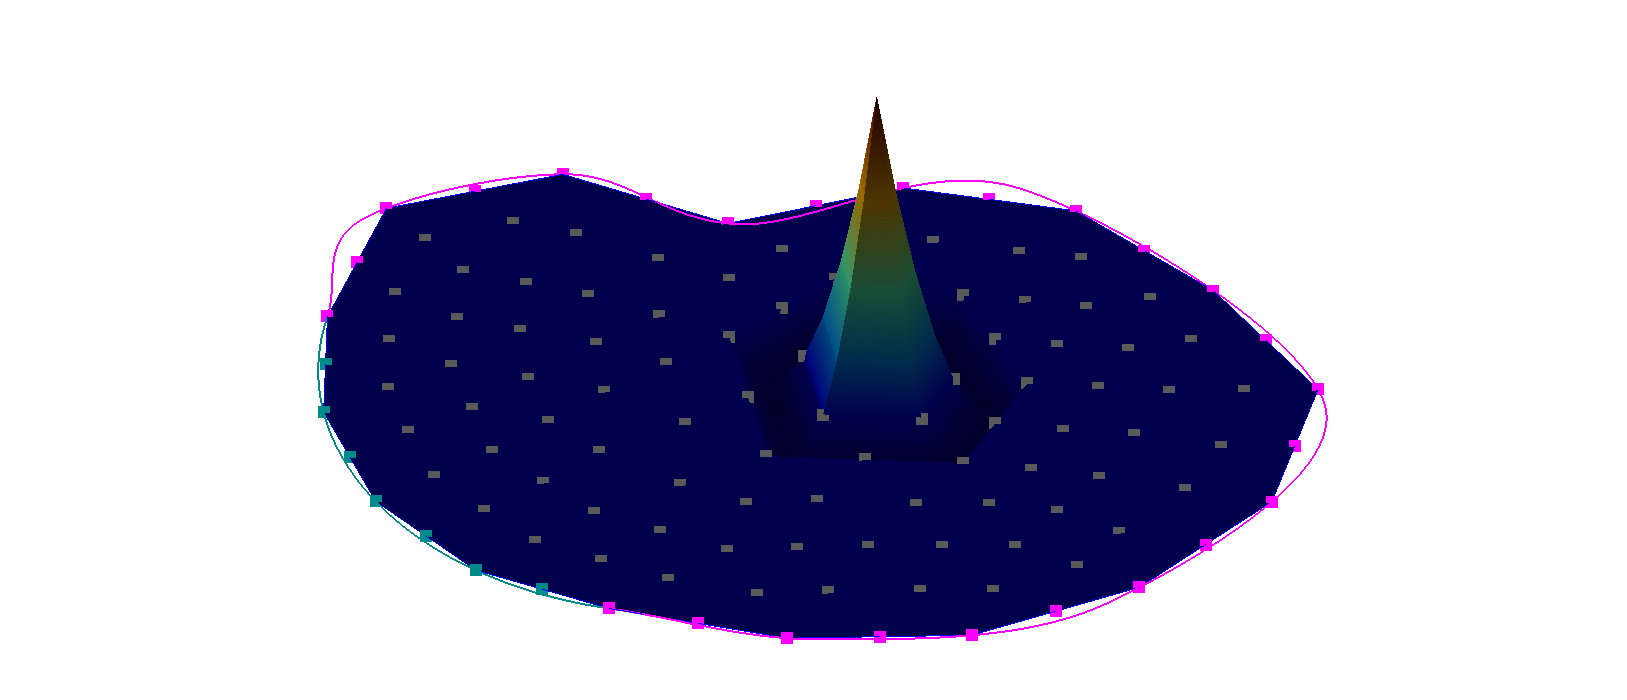
\includegraphics{040-discretizacion/shape-function-second-order-45.png}

}

}

\subcaption{\label{fig-shape-function-second-order-45}Nodo sobre una
esquina de un triángulo}
\end{minipage}%
%
\begin{minipage}[t]{0.05\linewidth}

{\centering 

~

}

\end{minipage}%
%
\begin{minipage}[t]{0.47\linewidth}

{\centering 

\raisebox{-\height}{

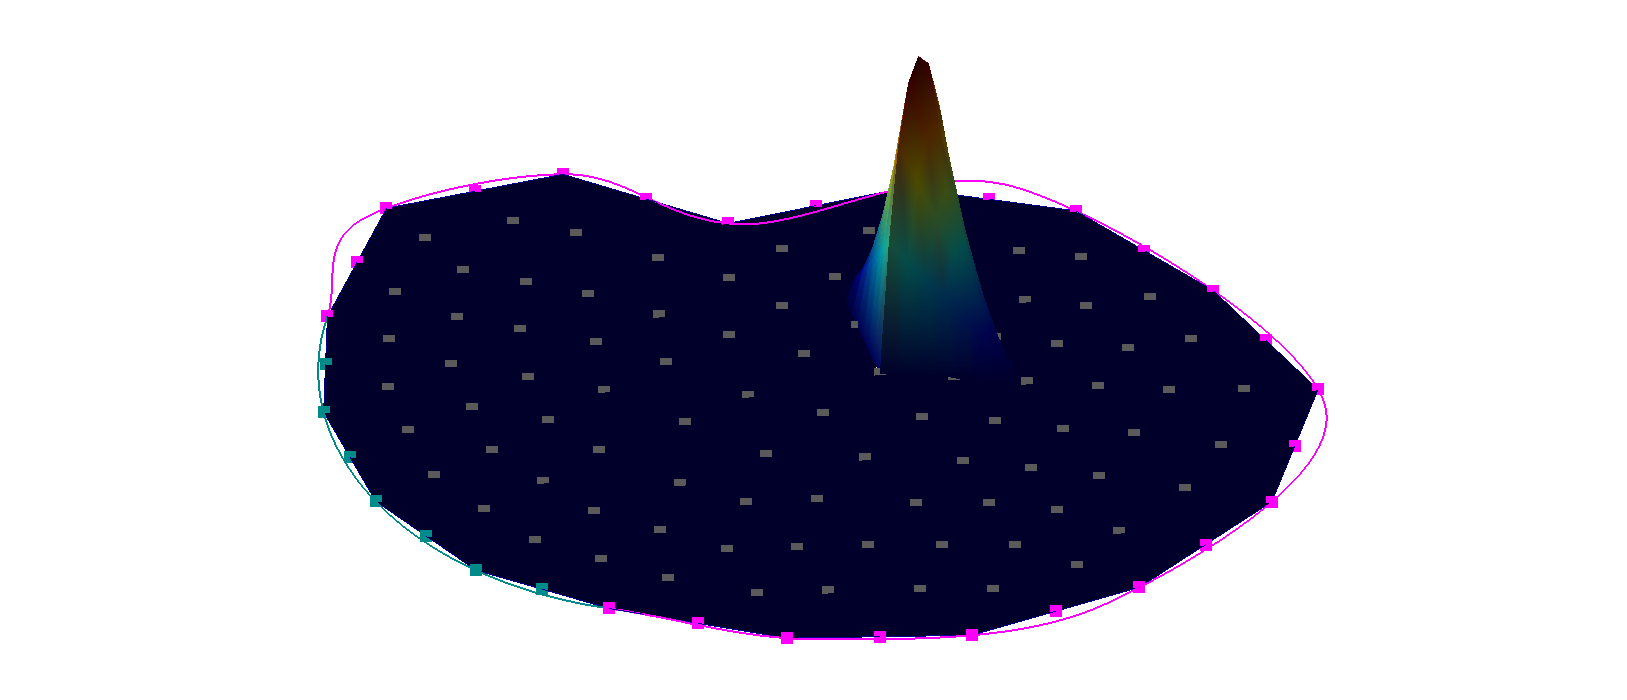
\includegraphics{040-discretizacion/shape-function-second-order-102.png}

}

}

\subcaption{\label{fig-shape-function-second-order-102}Nodo sobre un
borde de un triángulo}
\end{minipage}%

\caption{\label{fig-shape-function-second-order}Funciones de forma de
segundo orden tras agregar puntos en los bordes de los triángulos de
la~figura~\ref{fig-dominio-nodos-elementos}.}

\end{figure}

Para un problema de dimensión~\(D\), para cada elemento~\(e_i\) del
dominio discretizado~\(U \in \mathbb{R}^D\), una vez que conocemos

\begin{enumerate}
\def\labelenumi{\arabic{enumi}.}
\item
  la topología del elemento~\(e_i\)

  \begin{itemize}
  \tightlist
  \item
    segmento para~\(D=1\)
  \item
    triángulo o cuadrángulo para~\(D=2\)
  \item
    tetrahedro, hexahedro, prisma o pirámide para~\(D=3\)
  \end{itemize}
\item
  las~\(J\) funciones de forma~\(h_j(\symbf{\xi})\) del elemento
  canónico~\(e_c\) en el espacio~\(\symbf{\xi} \in \mathbb{R}^D\) con
  las cuales construimos la matriz~\(\mat{H}_c\) (\(G=1\) para un
  problema escalar){]}

  \[
  \mat{H}_c(\symbf{\xi}) = \begin{bmatrix}h_1(\symbf{\xi}) & h_2(\symbf{\xi}) & \cdots & h_J(\symbf{\xi}) \end{bmatrix} \quad \in \mathbb{R}^{G \times J}
  \]
\item
  las~\(J \times D\) derivadas parciales~\(\partial h_j/\partial \xi_d\)
  con respecto a las coordenadas~\(\symbf{\xi} \in \mathbb{R}^D\), con
  las cuales construimos la matriz~\(\mat{B}_c\)

  \[
  \mat{B}_c(\symbf{\xi}) =
  \begin{bmatrix}
  \frac{\partial h_1}{\partial \xi}   & \frac{\partial h_2}{\partial \xi}   & \cdots & \frac{\partial h_J}{\partial \xi} \\
  \frac{\partial h_1}{\partial \eta}  & \frac{\partial h_2}{\partial \eta}  & \cdots & \frac{\partial h_J}{\partial \eta} \\
  \frac{\partial h_1}{\partial \zeta} & \frac{\partial h_2}{\partial \zeta} & \cdots & \frac{\partial h_J}{\partial \zeta}
  \end{bmatrix} \quad \in \mathbb{R}^{D \times J}
  \]
\item
  el conjunto de~\(Q\) pares de pesos y ubicaciones de puntos de
  Gauss~\((\omega_q, \symbf{\xi}_q)\) del elemento canónico~\(e_c\)
\item
  las coordenadas reales~\(\vec{x}_j \in \mathbb{R}^D\) de los~\(J\)
  nodos que definen el elemento real~\(e_i\) con los que construimos la
  matriz de coordenadas~\(\mat{C}_i\)

  \[
  \mat{C}_i =
  \begin{bmatrix}
  x_1 & y_1 & z_1  \\
  x_2 & y_2 & z_2  \\
  \vdots & \vdots & \vdots  \\
  x_J & y_J & z_J  \\
  \end{bmatrix} \quad \in \mathbb{R}^{J \times D}
  \]

  que permite evaluar el jacobiano~\(\mat{J}(\symbf{\xi})\) como

  \begin{equation}\protect\hypertarget{eq-J-BC}{}{
  \mat{J}(\symbf{\xi}) = \mat{B}_c(\symbf{\xi}) \cdot \mat{C}_i
  }\label{eq-J-BC}\end{equation}

  y las coordenadas reales~\(\vec{x}_q\) de los~\(Q\) puntos de Gauss

  \[
  \begin{aligned}
  x_q &= \sum_{j=1}^J h_j(\symbf{\xi}_q) \cdot x_j \\
  y_q &= \sum_{j=1}^J h_j(\symbf{\xi}_q) \cdot y_j \\
  z_q &= \sum_{j=1}^J h_j(\symbf{\xi}_q) \cdot z_j \\
  \end{aligned}
  \]

  necesarias para evaluar~\(k(\vec{x})\) y \(f(\vec{x})\) dentro del
  integrando,
\end{enumerate}

entonces estamos en condiciones de evaluar la
matriz~\(K_i \in \mathbb{R}^{J \times J}\) de rigidez elemental
correspondiente a la formulación en elementos finitos\footnote{Estrictamente
  hablando, esta no es \emph{la} formulación sino que es una de las
  varias formulaciones posibles. De todas maneras es la más usual y
  eficiente.} de la ecuación generalizada de Poisson como

\[
\begin{aligned}
\mat{K}_i &= \int_{e_i} \mat{B}(\vec{x})^T \cdot k(\vec{x}) \cdot \mat{B}(\vec{x}) \, d^D\vec{x} \\
&= \int_{e_c} \mat{B}(\symbf{\xi})^T \cdot k(\symbf{\xi}) \cdot \mat{B}(\symbf{\xi}) \cdot \Big|\det{\left[\mat{J}\left(\symbf{\xi}\right)\right]}\Big| \, d^D\symbf{\xi} \\
&\approx
\sum_{q=1}^Q \omega_q \cdot \mat{B}(\symbf{\xi}_q)^T \cdot k(\symbf{\xi}_q) \cdot \mat{B}(\symbf{\xi}_q) \cdot \Big|\det{\left[\mat{J}\left(\symbf{\xi}_q\right)\right]}\Big| \\
&\approx
\sum_{q=1}^Q \omega_q \cdot \Big[ \mat{B}_c(\symbf{\xi}_q) \cdot \mat{J}^{-1}\left(\symbf{\xi}_q\right) \Big]^T k(\symbf{\xi}_q) \Big[ \mat{B}_c(\symbf{\xi}_q) \cdot \mat{J}^{-1}\left(\symbf{\xi}_q\right) \Big] \cdot \Big|\det{\left[\mat{J}\left(\symbf{\xi}_q\right)\right]}\Big| \\
\end{aligned}
\]

y la componente volumétrica del vector elemental~\(\vec{b}_i\) como

\[
\begin{aligned}
\vec{b}_i^{(U)} &= \int_{e_i} \mat{H}(\vec{x})^T \cdot f(\vec{x}) \, d^D\vec{x} \\
&= \int_{e_c} \mat{H}(\symbf{\xi})^T \cdot f(\symbf{\xi}) \cdot \Big|\det{\left[\mat{J}\left(\symbf{\xi}\right)\right]}\Big| \, d^D\symbf{\xi} \\
&\approx
\sum_{q=1}^Q \omega_q \cdot \mat{H}(\symbf{\xi}_q)^T \cdot f(\symbf{\xi}_q) \cdot \Big|\det{\left[\mat{J}\left(\symbf{\xi}_q\right)\right]}\Big| 
\end{aligned}
\]

Para evaluar las contribuciones de las condiciones de contorno
naturales, debemos integrar sobre elementos en la
frontera~\(\partial U\) del dominio~\(U\). Esto es, para~\(D=2\) debemos
integrar sobre elementos tipo segmento que están sobre el
plano~\(x\)-\(y\) (pero no necesariamente sobre la recta real).
Para~\(D=3\) debemos integrar sobre elementos triangulares o
cuadrangulares que están en el espacio~\(x\)-\(y\)-\(z\) (pero no
necesariamente sobre el plano~\(x\)-\(y\)). Hay varias formas de atacar
este problema. En esta tesis proponemos introducir una transformación
intermedia desde las coordenadas~\(\vec{x} \in \mathbb{R}^D\) hacia un
sistema de coordenadas~\(\vec{r} \in \mathbb{R}^{D-1}\), para luego sí
transformar las coordenadas~\(\vec{r}\) a \(\symbf{\xi}\) y realizar la
integración. Por ejemplo, si la condición de contorno de Neumann implica
integrar sobre un triángulo arbitrario cuyas coordenadas
son~\(\vec{x}_1\), \(\vec{x}_2\) y \(\vec{x}_3 \in \mathbb{R}^3\)
entonces primero encontramos una (de las infinitas)
rotaciones~\(\vec{x} \in \mathbb{R}^3 \mapsto \vec{r} \in \mathbb{R}^{2}\)
para luego
transformar~\(\vec{r} \in \mathbb{R}^{2} \mapsto \symbf{\xi} \in \mathbb{R}^{2}\)
y poder usar las matrices del elemento triangular canónico.

\begin{theorem}[]\protect\hypertarget{thm-rotacion}{}\label{thm-rotacion}

La matriz de rotación que lleva el vector~\(\vec{a} \in \mathbb{R}^3\)
al vector~\(\vec{b} \in \mathbb{R}^3\) es

\[
\mat{R} = \mat{I} + \mat{T} + \frac{1}{1 - \vec{a} \cdot \vec{b}} \cdot \mat{T}^2
\] donde la matriz~\(\mat{T}\) es

\[
\mat{T} = 
\begin{bmatrix}
0 & -\vec{t}_3 & +\vec{t}_2 \\
+\vec{t}_3 & 0 & -\vec{t}_1 \\
-\vec{t}_2 & +\vec{t}_1 & 0
\end{bmatrix}
\] y \(\vec{t}\) es producto cruz entre~\(\vec{a}\) y~\(\vec{b}\)

\[
\vec{t} = \vec{a} \times \vec{b}
\]

\end{theorem}

Lo que queremos es transformar una de las dos normales~\(\hat{\vec{n}}\)
del triángulo

\[
\hat{\vec{n}} = \frac{(\vec{x}_2 - \vec{x}_1) \times (\vec{x}_3 - \vec{x}_1)}{|| (\vec{x}_2 - \vec{x}_1) \times (\vec{x}_3 - \vec{x}_1) ||}
\]

para que coincida con versor normal en la dirección~\(z\),
\(\hat{\vec{e}}_z = [0,0,1]\). Haciendo~\(\vec{a} = \hat{\vec{n}}\)
y~\(\vec{b} = \hat{\vec{e}}_z\), el vector~\(\vec{t}\) es

\[
\begin{aligned}
\vec{t} &= \hat{\vec{n}} \times \hat{\vec{e}}_z \\
\end{aligned}
\]

Con esto podemos entonces convertir la matriz con las tres coordenadas
tridimensionales~\(\mat{C}_{3}\) del triángulo original a una de
coordenadas bidimensionales~\(\mat{C}_2\) como

\[
\begin{aligned}
\mat{C}_2 &= \mat{R} \cdot \mat{C}_3 \\
\begin{bmatrix}
x_1^\prime & x_2^\prime & x_3^\prime \\
y_1^\prime & y_2^\prime & y_3^\prime \\
0 & 0 & 0 \\
\end{bmatrix}
&=
\begin{bmatrix}
 1     + k \cdot (-\vec{t}_3^2- \vec{t}_2^2) &
 -\vec{t}_3 + k \cdot (\vec{t}_1\cdot \vec{t}_2) &
 +\vec{t}_2 + k \cdot (\vec{t}_1\cdot \vec{t}_3) \\
 +\vec{t}_3 + k \cdot (\vec{t}_1\cdot \vec{t}_2) &
 1     + k \cdot (-\vec{t}_3^2 - \vec{t}_1^2) &
 -\vec{t}_1 + k \cdot (\vec{t}_2\cdot \vec{t}_3) \\
 -\vec{t}_2 + k \cdot (\vec{t}_1\cdot \vec{t}_3) &
 +\vec{t}_1 + k \cdot (\vec{t}_2\cdot \vec{t}_3) &
 1     + k \cdot (-\vec{t}_2^2 - \vec{t}_1^2)
\end{bmatrix}
\cdot
\begin{bmatrix}
x_1 & x_2 & x_3 \\
y_1 & y_2 & y_3 \\
z_1 & z_2 & z_3
\end{bmatrix}
\end{aligned}
\] para

\[
k = \frac{1}{1- \hat{\vec{n}} \cdot \hat{\vec{e}}_z}
\]

Entonces podemos calcular el jacobiano de un elemento de superficie en
un problema tridimensional con las funciones de forma tradicionales del
triángulo canónico~\(e_c\). En efecto, la contribución de las
condiciones de contorno naturales al vector~\(b_i\) es entonces

\[
\begin{aligned}
\vec{b}_i^{(\Gamma_N)} &= \int_{e_i^{(D-1)}} \mat{H}(\vec{x})^T \cdot p(\vec{x}) \, d^{D-1}\vec{x} \\
&= \int_{e_c^{(D-1)}} \mat{H}(\symbf{\xi})^T \cdot p(\symbf{\xi}) \cdot \Big|\det{\left[\mat{J}\left(\symbf{\xi}\right)\right]}\Big| \, d^{D-1}\symbf{\xi} \\
&\approx
\sum_{q=1}^Q \omega_q^{(D-1)} \cdot \mat{H}(\symbf{\xi}_q)^T \cdot p(\symbf{\xi}_q) \cdot \Big|\det{\left[\mat{J}\left(\symbf{\xi}_q\right)\right]}\Big| 
\end{aligned}
\] donde la matriz~\(\vec{H}\) y el jacobiano~\(\mat{J}\) son los que le
corresponden al elemento de dimensión~\(D-1\).

\begin{remark}

Si no se hace nada, es como si~\(p(\vec{x})=0\).

\end{remark}

\hypertarget{sec-difusion-multigrupo-fem}{%
\subsection{Ecuación de difusión de
neutrones}\label{sec-difusion-multigrupo-fem}}

Estamos en condiciones entonces de discretizar en espacio las ecuaciones
de difusión multigrupo que derivamos en la~\textbf{?@sec-xxx}

\[ \tag{\ref{eq-difusionmultigrupo}}
\begin{gathered}
 - \text{div} \Big[ D_g(\vec{x}) \cdot \text{grad} \left[ \phi_g(\vec{x}) \right] \Big]
 + \Sigma_{t g}(\vec{x}) \cdot \phi_g(\vec{x})
 = \\
\sum_{g^\prime = 1}^G \Sigma_{s_0 g^\prime \rightarrow g}(\vec{x})  \cdot \phi_{g^\prime}(\vec{x}) +
\chi_g \sum_{g^\prime = 1}^G \nu\Sigma_{fg^\prime}(\vec{x}) \cdot \phi_{g^\prime}(\vec{x})+ s_{0g}(\vec{x})
\end{gathered}
\]

Comenzamos con el caso~\(G=1\) y luego generalizamos la formulación
para~\(G>1\).

\hypertarget{un-uxfanico-grupo-de-energuxeda}{%
\subsubsection{Un único grupo de
energía}\label{un-uxfanico-grupo-de-energuxeda}}

Para~\(G=1\) la ecuación se simplifica a

\[
 - \text{div} \Big[ D(\vec{x}) \cdot \text{grad} \left[ \phi(\vec{x}) \right] \Big]
 + \left[\Sigma_{t}(\vec{x})  - \Sigma_{s_0}(\vec{x}) - \nu\Sigma_{f}(\vec{x}) \right]\cdot \phi(\vec{x})
= s_{0}(\vec{x})
\]

El término de la divergencia y el miembro derecho tienen la misma forma
que la ecuación de Poisson, por lo que debemos esperar contribuciones
elementales~\(B^T D B\) y~\(H^T s_0\) respectivamente. Para evaluar el
término de fuente neta lineal con~\(\phi\) procedemos a multiplicar la
formulación fuerte por una función de
prueba~\(v(\vec{x}) \in V\)\footnote{Como para el problema de
  elasticidad al multiplicar la formulación fuerte por las funciones de
  prueba se obtiene el principio de los trabajos virtuales, a veces
  estas funciones de prueba se llaman ``desplazamientos virtuales''.
  Como generalización, en el problema de conducción de calor se las
  llaman ``temperaturas virtuales''. En este caso, podríamos llamarlas
  ``flujos escalares virtuales''.} e integrar en el
dominio~\(U\in\mathbb{R}^D\)

\[
\begin{gathered}
\int_U v(\vec{x}) \cdot \left\{ - \text{div} \Big[ D(\vec{x}) \cdot \text{grad} \left[ \phi(\vec{x}) \right] \Big] \right\} \, d^D\vec{x} \\
 + \int_U v(\vec{x}) \cdot \left\{ \left[\Sigma_{t}(\vec{x})  - \Sigma_{s_0}(\vec{x}) - \nu\Sigma_{f}(\vec{x}) \right] \cdot \phi(\vec{x}) \right\} \, d^D\vec{x}
= \int_U v(\vec{x}) \cdot s_{0}(\vec{x}) \, d^D\vec{x}
\end{gathered}
\]

Usando la fórmula de Green y el hecho de que~\(v(\vec{x})=0\)
en~\(\Gamma_D\) obtenemos la formulación débil de la ecuación de
difusión para un único grupo de energía

\[
\begin{gathered}
\int_U \text{grad} \left[ v(\vec{x}) \right] \cdot D(\vec{x}) \cdot \text{grad} \left[ \phi(\vec{x}) \right]  \,d^D\vec{x}
+ \int_U v(\vec{x}) \cdot \left[\Sigma_{t}(\vec{x})  - \Sigma_{s_0}(\vec{x}) - \nu\Sigma_{f}(\vec{x}) \right] \cdot \phi(\vec{x}) \,d^D\vec{x}
= \\
\int_U v(\vec{x}) \cdot s_0(\vec{x}) \,d^D\vec{x}
+ \int_{\Gamma_N} v(\vec{x}) \cdot p(\vec{x}) \,d^{D-1}\vec{x}
\end{gathered}
\] donde~\(p(\vec{x})\) es la condición de contorno de Neumann
sobre~\(\Gamma_D\)

\[
D(\vec{x}) \cdot \Big[ \text{grad} \left[ \phi(\vec{x}) \right] \cdot \hat{\vec{n}} \Big] = p(\vec{x})
\]

El operador bilineal~\(a(\phi,v)\) discretizado para este problema es

\[
\begin{aligned}
\mathcal{a}(\phi,v) =& \int_U \text{grad}\Big[ v(\vec{x}) \Big] \cdot D(\vec{x}) \cdot \text{grad}\Big[ \phi(\vec{x}) \Big] \, d^D \vec{x} \\
& \quad \quad + \int_U v(\vec{x}) \cdot \left[\Sigma_{t}(\vec{x})  - \Sigma_{s_0}(\vec{x}) - \nu\Sigma_{f}(\vec{x}) \right] \cdot \phi(\vec{x}) \,d^D\vec{x} \\
=& \int_U \vec{v}^T \cdot \mat{B}^T(\vec{x}) \cdot k(\vec{x}) \cdot \mat{B}(\vec{x}) \cdot \vec{u} \,\, d^D\vec{x}  \\
& \quad \quad + \int_U \vec{v}^T \cdot \mat{H}^T(\vec{x}) \cdot \left[\Sigma_{t}(\vec{x})  - \Sigma_{s_0}(\vec{x}) - \nu\Sigma_{f}(\vec{x}) \right] \cdot \mat{H}(\vec{x}) \cdot \symbf{\phi} \,\, d^D\vec{x} \\
&= \vec{v}^T \cdot \left[ \int_U \mat{B}^T(\vec{x}) \cdot k(\vec{x}) \cdot \mat{B}(\vec{x}) \, d^D\vec{x}
+ \int_U \mat{H}^T(\vec{x}) \cdot \left[\Sigma_{t}(\vec{x})  - \Sigma_{s_0}(\vec{x}) - \nu\Sigma_{f}(\vec{x}) \right] \cdot \mat{H}(\vec{x})
\right] \cdot \symbf{\phi} \\
\end{aligned}
\]

Podemos escribimos la matriz de rigidez elemental~\(K_i\) como

\[
\mat{K}_i = 
\sum_{q=1}^Q \omega_q \cdot \left[ \mat{L}_i(\symbf{\xi}_q) + \mat{A}_i(\symbf{\xi}_q) - \mat{F}_i(\symbf{\xi}_q)\right] \cdot \Big|\det{\left[\mat{J}\left(\symbf{\xi}_q\right)\right]}\Big|
\]

donde tenemos la matriz elemental de ``pérdidas''\footnote{Del inglés
  \foreignlanguage{american}{\emph{leakage}}.}

\[
\mat{L}_i = \Big[ \mat{B}_c(\symbf{\xi}_q) \cdot \mat{J}^{-1}\left(\symbf{\xi}_q\right) \Big]^T \cdot D(\symbf{\xi}_q) \cdot \Big[ \mat{B}_c(\symbf{\xi}_q) \cdot \mat{J}^{-1}\left(\symbf{\xi}_q\right) \Big]
\] la matriz elemental de absorciones

\[
\mat{A}_i = \mat{H}_c(\symbf{\xi}_q)^T \cdot \left[ \Sigma_t(\symbf{\xi}_q) - \Sigma_{s_0} (\symbf{\xi}_q) \right] \cdot \mat{H}_c(\symbf{\xi}_q)
\] y la matriz elemental de fisiones

\[
\mat{F}_i = \mat{H}_c(\symbf{\xi}_q)^T \cdot \nu\Sigma_f(\symbf{\xi}_q) \cdot \mat{H}_c(\symbf{\xi}_q)
\]

De la misma manera, el funcional~\(\mathcal{B}(v)\) es \[
\begin{aligned}
\mathcal{B}(v) &= \int_U v(\vec{x}) \cdot s_0(\vec{x}) \, d^D \vec{x} + \int_{\Gamma_N} v(\vec{x}) \cdot p(\vec{x}) \, d^{D-1} \vec{x} \\
&= \int_U \vec{v}^T \cdot \mat{H}^T(\vec{x}) \cdot s_0(\vec{x}) \, d^D \vec{x}
+ \int_{\Gamma_N} \vec{v}^T \cdot \mat{H}^T(\vec{x}) \cdot p(\vec{x}) \, d^{D-1} \vec{x} \\
&= \vec{v}^T \cdot \left[ \int_{U} \mat{H}^T(\vec{x}) \cdot s_0(\vec{x}) \, d^D \vec{x}
+ \int_{\Gamma_N} \mat{H}^T(\vec{x}) \cdot p(\vec{x}) \, d^{D-1}\vec{x} \right]
\end{aligned}
\] y las contribuciones volumétricas y superficiales al
vector~\(\vec{b}_i\) son similares al caso del problema de Poisson

\[
\begin{aligned}
\vec{b}_i^{(U)} &= \int_{e_i} \mat{H}(\vec{x})^T \cdot s_0(\vec{x}) \, d^D\vec{x} \\
&= \int_{e_c} \mat{H}(\symbf{\xi})^T \cdot s_0(\symbf{\xi}) \cdot \Big|\det{\left[\mat{J}\left(\symbf{\xi}\right)\right]}\Big| \, d^D\symbf{\xi} \\
&\approx
\sum_{q=1}^Q \omega_q \cdot \mat{H}(\symbf{\xi}_q)^T \cdot s_0(\symbf{\xi}_q) \cdot \Big|\det{\left[\mat{J}\left(\symbf{\xi}_q\right)\right]}\Big| 
\end{aligned}
\] y \[
\begin{aligned}
\vec{b}_i^{(\Gamma_N)} &= \int_{e_i^{(D-1)}} \mat{H}(\vec{x})^T \cdot p(\vec{x}) \, d^{D-1}\vec{x} \\
&= \int_{e_c^{(D-1)}} \mat{H}(\symbf{\xi})^T \cdot p(\symbf{\xi}) \cdot \Big|\det{\left[\mat{J}\left(\symbf{\xi}\right)\right]}\Big| \, d^{D-1}\symbf{\xi} \\
&\approx
\sum_{q=1}^Q \omega_q^{(D-1)} \cdot \mat{H}(\symbf{\xi}_q)^T \cdot p(\symbf{\xi}_q) \cdot \Big|\det{\left[\mat{J}\left(\symbf{\xi}_q\right)\right]}\Big| 
\end{aligned}
\] respectivamente.

\hypertarget{grupos-arbitrarios-de-energuxeda}{%
\subsubsection{Grupos arbitrarios de
energía}\label{grupos-arbitrarios-de-energuxeda}}

Consideremos el caso~\(G=2\). La formulación fuerte son dos ecuaciones
diferenciales en derivadas parciales acopladas entre sí a través de los
términos de \foreignlanguage{american}{scattering} y de fisión

\[
\begin{cases}
 - \text{div} \left[ D_1 \, \text{grad} \left( \phi_1 \right) \right]
 + \Sigma_{t1} \phi_1 - \Sigma_{s_0 1 \rightarrow 1} \phi_1 - \Sigma_{s_0 2 \rightarrow 1} \phi_2 - \chi_1 \left[ \nu\Sigma_{f1} \phi_1 + \nu\Sigma_{f2} \phi_2 \right] = s_{0,1} \\
 - \text{div} \left[ D_2 \, \text{grad} \left( \phi_2 \right) \right]
 + \Sigma_{t2} \phi_2 - \Sigma_{s_0 1 \rightarrow 2} \phi_1 - \Sigma_{s_0 2 \rightarrow 2} \phi_2 - \chi_2 \left[ \nu\Sigma_{f1} \phi_1 + \nu\Sigma_{f2} \phi_2 \right] = s_{0,2}
\end{cases}
\] que podemos escribir en una ecuación vectorial como

\[
\begin{gathered}
\begin{bmatrix}
 - \text{div} \left[ D_1(\vec{x}) \, \text{grad} \left( \phi_1 \right) \right] \\
 - \text{div} \left[ D_2(\vec{x}) \, \text{grad} \left( \phi_2 \right) \right] \\
\end{bmatrix}
+
\begin{bmatrix}
 \Sigma_{t1}(\vec{x}) - \Sigma_{s_0 1 \rightarrow 1}(\vec{x}) & - \Sigma_{s_0 2 \rightarrow 1}(\vec{x}) \\
 - \Sigma_{s_0 1 \rightarrow 2}(\vec{x}) & \Sigma_{t2}(\vec{x}) - \Sigma_{s_0 2 \rightarrow 2}(\vec{x}) \\
\end{bmatrix}
\cdot
\begin{bmatrix}
 \phi_1(\vec{x}) \\
 \phi_2(\vec{x}) \\
\end{bmatrix}
\\
-
\begin{bmatrix}
 \chi_1 \cdot \nu\Sigma_{f1}(\vec{x}) & \chi_1 \cdot \nu\Sigma_{f2}(\vec{x}) \\
 \chi_2 \cdot \nu\Sigma_{f1}(\vec{x}) & \chi_2 \cdot \nu\Sigma_{f2}(\vec{x}) \\
\end{bmatrix}
\cdot
\begin{bmatrix}
 \phi_1(\vec{x}) \\
 \phi_2(\vec{x}) \\
\end{bmatrix}
=
\begin{bmatrix}
 s_{0,1}(\vec{x}) \\
 s_{0,2}(\vec{x}) \\
\end{bmatrix}
\end{gathered}
\]

Introduciendo la matriz~\(\mat{R} \in \mathbb{R}^{G \times G}\) de
remociones

\[
\mat{R}(\vec{x}) =
\begin{bmatrix}
 \Sigma_{t1}(\vec{x}) & 0 \\
 0 & \Sigma_{t2}(\vec{x}) \\
\end{bmatrix}
-
\begin{bmatrix}
 \Sigma_{s_0 1 \rightarrow 1}(\vec{x}) & \Sigma_{s_0 2 \rightarrow 1}(\vec{x}) \\
 \Sigma_{s_0 1 \rightarrow 2}(\vec{x}) & \Sigma_{s_0 2 \rightarrow 2}(\vec{x}) \\
\end{bmatrix}
\] y la matrix~\(\mat{X} \in \mathbb{R}^{G \times G}\) de nu-fisiones

\[
\mat{X}(\vec{x}) =
\begin{bmatrix}
 \chi_1 \cdot \nu\Sigma_{f1}(\vec{x}) & \chi_1 \cdot \nu\Sigma_{f2}(\vec{x}) \\
 \chi_2 \cdot \nu\Sigma_{f1}(\vec{x}) & \chi_2 \cdot \nu\Sigma_{f2}(\vec{x}) \\
\end{bmatrix}
\] la formulación fuerte para~\(G=2\) queda

\[
\begin{bmatrix}
 - \text{div} \left[ D_1(\vec{x}) \, \text{grad} \left( \phi_1 \right) \right] \\
 - \text{div} \left[ D_2(\vec{x})\, \text{grad} \left( \phi_2 \right) \right] \\
\end{bmatrix}
+
\mat{R}(\vec{x})
\cdot
\begin{bmatrix}
 \phi_1(\vec{x}) \\
 \phi_2(\vec{x}) \\
\end{bmatrix}
-
\mat{X}(\vec{x})
\cdot
\begin{bmatrix}
 \phi_1(\vec{x}) \\
 \phi_2(\vec{x}) \\
\end{bmatrix}
=
\begin{bmatrix}
 s_{0,1}(\vec{x}) \\
 s_{0,2}(\vec{x}) \\
\end{bmatrix}
\]

Para encontrar la formulación débil multiplicamos cada una de las dos
ecuaciones por funciones de prueba~\(v_1(\vec{x}) \in V\)
y~\(v_2(\vec{x}) \in V\) respectivamente, las sumamos, integramos en el
dominio~\(U \in \mathbb{R}^D\) y aplicamos la fórmula de Green al
término de la divergencia:

\[
\begin{gathered}
\bigintsss_U
\begin{bmatrix}
 \nabla v_1 & \nabla v_2
\end{bmatrix}
\cdot
\begin{bmatrix}
D_1(\vec{x}) & 0 \\
0 & D_2(\vec{x}) \\
\end{bmatrix}
\cdot
\begin{bmatrix}
\nabla \phi_1  \\
\nabla \phi_2  \\
\end{bmatrix}
\, d^D\vec{x}
+
\bigintsss_U
\begin{bmatrix}
 v_1 & v_2
\end{bmatrix}
\cdot
\Big[\mat{R}(\vec{x}) - \mat{X}(\vec{x})\Big]
\cdot
\begin{bmatrix}
 \phi_1(\vec{x}) \\
 \phi_2(\vec{x}) \\
\end{bmatrix}
\, d^D\vec{x}
\\
=
\bigintsss_U
\begin{bmatrix}
 v_1 & v_2
\end{bmatrix}
\cdot
\begin{bmatrix}
 s_{0,1}(\vec{x}) \\
 s_{0,2}(\vec{x}) \\
\end{bmatrix}
\, d^D\vec{x}
+
\bigintsss_{\Gamma_D}
\begin{bmatrix}
 v_1 & v_2
\end{bmatrix}
\cdot
\begin{bmatrix}
 p_1(\vec{x}) \\
 p_2(\vec{x}) \\
\end{bmatrix}
\, d^{D-1}\vec{x}
\end{gathered}
\]

Si definimos un vector~\(\vec{v} \in \mathbb{R}^{GJ}\) con los valores
nodales de~\(v_1(\vec{x})\) y~\(v_2(\vec{x})\) intercalados

\[
\vec{v} =
\begin{bmatrix}
 v_1^{(1)} \\ v_2^{(1)} \\
 v_1^{(1)} \\ v_2^{(1)} \\
\vdots \\
 v_1^{(J)} \\ v_2^{(J)} \\
\end{bmatrix}
\] entonces

\[
\begin{bmatrix}
 v_1(\vec{x}) \\ v_2(\vec{x})
\end{bmatrix}
=
\mat{H}(\vec{x})
\cdot
\vec{v}
\] con

\[
\mat{H}(\vec{x}) =
\begin{bmatrix}
h_1(\vec{x}) & 0 & h_2(\vec{x}) & 0 & \cdots & h_J(\vec{x}) & 0 \\
0 & h_1(\vec{x}) & 0 & h_2(\vec{x}) & \cdots & 0 & h_J(\vec{x}) \\
\end{bmatrix} \quad \in \mathbb{R}^{G \times JG}
\]

De la misma manera, si

\[
\symbf{\phi} =
\begin{bmatrix}
 \phi_1^{(1)} \\ \phi_2^{(1)} \\
 \phi_1^{(1)} \\ \phi_2^{(1)} \\
\vdots \\
 \phi_1^{(J)} \\ \phi_2^{(J)} \\
\end{bmatrix}
\] entonces

\[
\begin{bmatrix}
 \phi_1(\vec{x}) \\ \phi_2(\vec{x})
\end{bmatrix}
=
\mat{H}(\vec{x})
\cdot
\symbf{\phi}
\] y el término de remociones menos fisiones queda

\[
\bigintsss_U
\begin{bmatrix}
 v_1 & v_2
\end{bmatrix}
\cdot
\Big[\mat{R}(\vec{x}) - \mat{X}(\vec{x})\Big]
\cdot
\begin{bmatrix}
 \phi_1(\vec{x}) \\
 \phi_2(\vec{x}) \\
\end{bmatrix}
\, d^D\vec{x}
=
\vec{v}^T
\cdot
\left[
\int_U
\mat{H}^T
\cdot
\Big[\mat{R}(\vec{x}) - \mat{X}(\vec{x})\Big]
\cdot
\mat{H}^T
\, d^D\vec{x}
\right]
\cdot
\symbf{\phi}
\]

El término de fuentes volumétricas del miembro derecho queda

\[
\bigintsss_U
\begin{bmatrix}
 v_1 & v_2
\end{bmatrix}
\cdot
\begin{bmatrix}
 s_{0,1}(\vec{x}) \\
 s_{0,2}(\vec{x}) \\
\end{bmatrix}
\, d^D\vec{x}
=
\vec{v}^T
\cdot
\left[
\int_U
\mat{H}^T
\cdot
\begin{bmatrix}
 s_{0,1}(\vec{x}) \\
 s_{0,2}(\vec{x}) \\
\end{bmatrix}
\, d^D\vec{x}
\right]
\] y el de condiciones de contorno naturales

\[
\bigintsss_{\Gamma_D}
\begin{bmatrix}
 v_1 & v_2
\end{bmatrix}
\cdot
\begin{bmatrix}
 p_1(\vec{x}) \\
 p_2(\vec{x}) \\
\end{bmatrix}
\, d^{D-1}\vec{x}
=
\vec{v}^T
\cdot
\left[
\int_{\Gamma_N}
\mat{H}^T
\cdot
\begin{bmatrix}
 p_1(\vec{x}) \\
 p_2(\vec{x}) \\
\end{bmatrix}
\, d^{D-1}\vec{x}
\right]
\]

Nos queda evaluar el término de pérdidas. Para ello por un lado notamos
que

\[
\begin{aligned}
\begin{bmatrix}
 \nabla v_1 & \nabla v_2
\end{bmatrix}
\cdot
\begin{bmatrix}
D_1(\vec{x}) & 0 \\
0 & D_2(\vec{x}) \\
\end{bmatrix}
\cdot
\begin{bmatrix}
\nabla \phi_1  \\
\nabla \phi_2  \\
\end{bmatrix}
=&
   \frac{\partial v_1}{\partial x} \cdot D_1 \cdot \frac{\partial \phi_1}{\partial x}
 + \frac{\partial v_2}{\partial x} \cdot D_2 \cdot \frac{\partial \phi_2}{\partial x} \\
&~
 + \frac{\partial v_1}{\partial y} \cdot D_1 \cdot \frac{\partial \phi_1}{\partial y}
 + \frac{\partial v_2}{\partial y} \cdot D_2 \cdot \frac{\partial \phi_2}{\partial y} \\
=&
\begin{bmatrix}
\frac{\partial v_1}{\partial x} &
\frac{\partial v_2}{\partial x} &
\frac{\partial v_1}{\partial y} &
\frac{\partial v_2}{\partial y}
\end{bmatrix}
\begin{bmatrix}
D_1 & 0 & 0 & 0 \\
0 & D_2 & 0 & 0 \\
0 & 0 & D_1 & 0 \\
0 & 0 & 0 & D_2 \\
\end{bmatrix}
\begin{bmatrix}
\frac{\partial \phi_1}{\partial x} \\
\frac{\partial \phi_2}{\partial x} \\
\frac{\partial \phi_1}{\partial y} \\
\frac{\partial \phi_2}{\partial y}
\end{bmatrix}
\end{aligned}
\] y por el otro que

\[
\begin{bmatrix}
\frac{\partial v_1}{\partial x} \\
\frac{\partial v_2}{\partial x} \\
\frac{\partial v_1}{\partial y} \\
\frac{\partial v_2}{\partial y}
\end{bmatrix}
=
\mat{B}(\vec{x}) \cdot \vec{v}
\quad\quad\quad
\begin{bmatrix}
\frac{\partial \phi_1}{\partial x} \\
\frac{\partial \phi_2}{\partial x} \\
\frac{\partial \phi_1}{\partial y} \\
\frac{\partial \phi_2}{\partial y}
\end{bmatrix}
=
\mat{B}(\vec{x}) \cdot \symbf{\phi}
\] con

\[
\mat{B}(\vec{x}) =
\begin{bmatrix}
\frac{\partial h_1}{\partial x}   & 0 & \frac{\partial h_2}{\partial x}   & 0  & \cdots & \frac{\partial h_J}{\partial x} & 0 \\
0 & \frac{\partial h_1}{\partial x}  & 0 & \frac{\partial h_2}{\partial x} &  \cdots & 0 & \frac{\partial h_J}{\partial x}  \\
\frac{\partial h_1}{\partial y}  & 0 & \frac{\partial h_2}{\partial y}  & 0 & \cdots & \frac{\partial h_J}{\partial y} & 0 \\
0 & \frac{\partial h_1}{\partial y}  & 0 & \frac{\partial h_2}{\partial y}  & \cdots & 0 & \frac{\partial h_J}{\partial y} \\
\frac{\partial h_1}{\partial z} & 0 & \frac{\partial h_2}{\partial z} & 0 & \cdots & \frac{\partial h_J}{\partial z} & 0 \\
0 & \frac{\partial h_1}{\partial z} & 0 & \frac{\partial h_2}{\partial z}  & \cdots & 0 & \frac{\partial h_J}{\partial z} \\
\end{bmatrix} \quad \in \mathbb{R}^{D \times JG}
\] entonces

\[
\bigintsss_U
\begin{bmatrix}
 \nabla v_1 & \nabla v_2
\end{bmatrix}
\cdot
\begin{bmatrix}
D_1(\vec{x}) & 0 \\
0 & D_2(\vec{x}) \\
\end{bmatrix}
\cdot
\begin{bmatrix}
\nabla \phi_1  \\
\nabla \phi_2  \\
\end{bmatrix}
\, d^D\vec{x}
=
\vec{v}^T
\cdot
\left[
\int_U
\mat{B}^T(\vec{x})
\cdot
\mat{D}^{\prime}(\vec{x})
\cdot
\mat{B}(\vec{x})
\, d^D\vec{x}
\right]
\cdot
\symbf{\phi}
\] siendo las matrices~\(\mat{D} \in \mathbb{R}^{G \times G}\) y
\(\mat{D}^{\prime} \in \mathbb{R}^{GD \times GD}\)

\[
\mat{D}(\vec{x}) =
\begin{bmatrix}
D_1(\vec{x}) & 0 \\
0 & D_2(\vec{x}) \\
\end{bmatrix}
\]

\[
\mat{D}^\prime(\vec{x}) =
\begin{bmatrix}
\mat{D}(\vec{x}) & \mat{0} \\
\mat{0} & \mat{D}(\vec{x}) \\
\end{bmatrix}
=
\begin{bmatrix}
D_1(\vec{x}) & 0 & 0 & 0 \\
0 & D_2(\vec{x}) & 0 & 0 \\
0 & 0 & D_1(\vec{x}) & 0 \\
0 & 0 & 0 & D_2(\vec{x}) \\
\end{bmatrix}
\]

Juntando estos resultados, el problema de Galerkin para difusión de
neutrones a~\(G=2\) grupos es
encontrar~\(\symbf{\phi} \in \mathbb{R}^{JG}\) tal que

\[
\begin{gathered}
\vec{v}^T \cdot
\left[
\int_U
\Big\{
\mat{B}^T(\vec{x})
\cdot
\mat{D}^{\prime}(\vec{x})
\cdot
\mat{B}(\vec{x})
+
\mat{H}^T(\vec{x})
\cdot
\left[ \mat{R}(\vec{x})-\mat{F}(\vec{x})\right]
\cdot
\mat{H}(\vec{x})
\Big\}
\, d^D\vec{x}
\right]
\cdot
\symbf{\phi}
=\\
\vec{v}^T \cdot
\left[
\int_U
\mat{H}^T
\cdot
\begin{bmatrix}
 s_{0,1}(\vec{x}) \\
 s_{0,2}(\vec{x}) \\
\end{bmatrix}
\, d^D\vec{x}
+
\int_{\Gamma_N}
\mat{H}^T
\cdot
\begin{bmatrix}
 p_1(\vec{x}) \\
 p_2(\vec{x}) \\
\end{bmatrix}
\, d^{D-1}\vec{x}
\right]
\end{gathered}
\] para todo~\(\vec{v}\in \mathbb{R}^{JG}\).

Luego, para el caso general de~\(G\) grupos de energía podemos escribir
la matriz de rigidez elemental~\(\mat{K}_i\) como \[
\begin{aligned}
\mat{K}_i &= 
\sum_{q=1}^Q \omega_q \cdot \left[ \mat{L}_i(\symbf{\xi}_q) + \mat{A}_i(\symbf{\xi}_q) - \mat{F}_i(\symbf{\xi}_q)\right] \cdot \Big|\det{\left[\mat{J}\left(\symbf{\xi}_q\right)\right]}\Big|
\end{aligned}
\]

a partir de las matrices elementales de pérdidas, absorciones y fisiones

\[
\begin{aligned}
\mat{L}_i &= \Big[ \mat{B}_c(\symbf{\xi}_q) \cdot \mat{J}^{-1}\left(\symbf{\xi}_q\right) \Big]^T \cdot \mat{D}(\symbf{\xi}_q) \cdot \Big[ \mat{B}_c(\symbf{\xi}_q) \cdot \mat{J}^{-1}\left(\symbf{\xi}_q\right) \Big] \\
\mat{A}_i &= \mat{H}_c(\symbf{\xi}_q)^T \cdot \mat{R}(\symbf{\xi}_q) \cdot \mat{H}_c(\symbf{\xi}_q) \\
\mat{F}_i &= \mat{H}_c(\symbf{\xi}_q)^T \cdot \mat{X}(\symbf{\xi}_q) \cdot \mat{H}_c(\symbf{\xi}_q)
\end{aligned}
\] para las matrices de forma elementales

\[
\mat{H}_c(\symbf{\xi}) =
\begin{bmatrix}
h_1(\symbf{\xi}) & 0 & h_2(\symbf{\xi}) & 0 & \cdots & h_J(\symbf{\xi}) & 0 \\
0 & h_1(\symbf{\xi}) & 0 & h_2(\symbf{\xi}) & \cdots & 0 & h_J(\symbf{\xi}) \\
\end{bmatrix} \quad \in \mathbb{R}^{G \times JG}
\] y

\[
\mat{B}_c(\symbf{\xi}) =
\begin{bmatrix}
\frac{\partial h_1}{\partial \xi}   & 0 & \frac{\partial h_2}{\partial \xi}   & 0  & \cdots & \frac{\partial h_J}{\partial \xi} & 0 \\
0 & \frac{\partial h_1}{\partial \xi}  & 0 & \frac{\partial h_2}{\partial \xi} &  \cdots & 0 & \frac{\partial h_J}{\partial \xi}  \\
\frac{\partial h_1}{\partial \eta}  & 0 & \frac{\partial h_2}{\partial \eta}  & 0 & \cdots & \frac{\partial h_J}{\partial \eta} & 0 \\
0 & \frac{\partial h_1}{\partial \eta}  & 0 & \frac{\partial h_2}{\partial \eta}  & \cdots & 0 & \frac{\partial h_J}{\partial \eta} \\
\frac{\partial h_1}{\partial \zeta} & 0 & \frac{\partial h_2}{\partial \zeta} & 0 & \cdots & \frac{\partial h_J}{\partial \zeta} & 0 \\
0 & \frac{\partial h_1}{\partial \zeta} & 0 & \frac{\partial h_2}{\partial \zeta}  & \cdots & 0 & \frac{\partial h_J}{\partial \zeta} \\
\end{bmatrix} \quad \in \mathbb{R}^{D \times JG}
\] con las matrices de secciones eficaces macroscópicas de difusión,
remoción y nu-fisión

\[
\begin{aligned}
\mat{D}(\vec{x}) &=
\begin{bmatrix}
D_1(\vec{x}) & 0 & \cdots & 0 \\
0 & D_2(\vec{x}) & \cdots & 0 \\
\vdots & \vdots & \ddots & \vdots \\
0 & 0 & \cdots & D_G(\vec{x})
\end{bmatrix} \in \mathbb{R}^{G \times G}
\\
\mat{D}^{\prime}(\vec{x}) &=
\begin{bmatrix}
\mat{D}(\vec{x}) & \mat{0} & \cdots & \mat{0} \\
\mat{0} & \mat{D}(\vec{x}) & \cdots & \mat{0} \\
\vdots & \vdots & \ddots & \vdots \\
\mat{0} & \mat{0} & \cdots & \mat{D}(\vec{x})
\end{bmatrix} \in \mathbb{R}^{GD \times GD}
\\
\mat{R} &=
\begin{bmatrix}
\Sigma_{t1}(\vec{x}) & 0 & \cdots & 0 \\
0 & \Sigma_{t2}(\vec{x}) & \cdots & 0 \\
\vdots & \vdots & \ddots & \vdots \\
0 & 0 & \cdots & \Sigma_{tG}(\vec{x})
\end{bmatrix}
-
\begin{bmatrix}
\Sigma_{s_0 1 \rightarrow 1}(\vec{x}) & \Sigma_{s_0 2 \rightarrow 1} & \cdots & \Sigma_{s_0 G \rightarrow 1} \\
\Sigma_{s_0 1 \rightarrow 2}(\vec{x}) & \Sigma_{s_0 2 \rightarrow 2} & \cdots & \Sigma_{s_0 G \rightarrow 2} \\
\vdots & \vdots & \ddots & \vdots \\
\Sigma_{s_0 1 \rightarrow G}(\vec{x}) & \Sigma_{s_0 2 \rightarrow G} & \cdots & \Sigma_{s_0 G \rightarrow G} \\
\end{bmatrix} \in \mathbb{R}^{G \times G}
\\
\mat{X} &=
\begin{bmatrix}
\chi_1 \cdot \nu\Sigma_{f1}(\vec{x}) & \chi_1 \cdot \nu\Sigma_{f2}(\vec{x}) & \cdots & \chi_1 \cdot \nu\Sigma_{fG}(\vec{x}) \\
\chi_2 \cdot \nu\Sigma_{f1}(\vec{x}) & \chi_2 \cdot \nu\Sigma_{f2}(\vec{x}) & \cdots & \chi_2 \cdot \nu\Sigma_{fG}(\vec{x}) \\
\vdots & \vdots & \ddots & \vdots \\
\chi_G \cdot \nu\Sigma_{f1}(\vec{x}) & \chi_G \cdot \nu\Sigma_{f2}(\vec{x}) & \cdots & \chi_G \cdot \nu\Sigma_{fG}(\vec{x}) \\
\end{bmatrix} \in \mathbb{R}^{G \times G}
\end{aligned}
\]

\hypertarget{sec-sn-multigrupo-fem}{%
\subsection{Ordenadas discretas
multigrupo}\label{sec-sn-multigrupo-fem}}

Ultricies lacus sed turpis tincidunt id. Elementum pulvinar etiam non
quam lacus suspendisse faucibus. Tortor consequat id porta nibh. Eu
lobortis elementum nibh tellus molestie nunc non. Facilisis gravida
neque convallis a cras semper auctor neque vitae. Nisl purus in mollis
nunc sed id semper risus in. Mattis nunc sed blandit libero. Consectetur
adipiscing elit duis tristique sollicitudin nibh sit amet commodo.
Faucibus purus in massa tempor nec. Arcu odio ut sem nulla pharetra diam
sit. Tempus imperdiet nulla malesuada pellentesque elit eget gravida cum
sociis. Vitae semper quis lectus nulla at volutpat diam. Gravida arcu ac
tortor dignissim convallis. Est velit egestas dui id ornare arcu odio.
Odio facilisis mauris sit amet massa vitae. Nibh cras pulvinar mattis
nunc sed blandit libero volutpat.

\hypertarget{sec-problemas-steady-state}{%
\section{Problemas de estado
estacionario}\label{sec-problemas-steady-state}}

Si bien en el~\textbf{?@sec-transporte-difusion} hemos mantenido por
completitud la dependencia temporal explícitamente en los flujos y
corrientes, en esta tesis resolvemos solamente problemas de estado
estacionario. Al eliminar el término de la temporada con respecto al
tiempo, las propiedades matemáticas de las ecuaciones cambian y por lo
tanto debemos resolverlas en forma diferente según tengamos alguno de
los siguientes tres casos:

\begin{enumerate}
\tightlist
\item
  Medio no multiplicativo con fuentes independientes,
\item
  Medio multiplicativo con fuentes independientes, y
\item
  Medio multiplicativo sin fuentes independientes.
\end{enumerate}

\hypertarget{sec-nomult-src}{%
\subsection{Medio no multiplicativo con fuentes
independientes}\label{sec-nomult-src}}

Un medio no multiplicativo es aquel que no contiene núcleos capaces de
fisionar. Cada neutrón que encontremos en el medio debe entonces
provenir de una fuente externa~\(s\). Para estudiar este tipo de
problemas, además de eliminar la derivada temporal y la dependencia con
el tiempo, tenemos que hacer cero el término de fisión. Luego la
ecuación de difusión queda

\begin{equation}\protect\hypertarget{eq-difusionnmfi}{}{
\begin{gathered}
 - \text{div} \Big[ D(\vec{x}, E) \cdot \text{grad} \left[ \phi(\vec{x}, E) \right] \Big]
 + \Sigma_t(\vec{x}, E) \cdot \phi(\vec{x}, E)
 = \\
\int_{0}^{\infty} \Sigma_{s_0}(\vec{x}, E^{\prime} \rightarrow E)  \cdot \phi(\vec{x}, E^\prime) \, dE^\prime
+ s_0(\vec{x}, E)
\end{gathered}
}\label{eq-difusionnmfi}\end{equation} y la de transporte

\begin{equation}\protect\hypertarget{eq-transportenmfi}{}{ 
\begin{gathered}
 \omegaversor \cdot \text{grad} \left[ \psi(\vec{x}, \omegaversor, E) \right]
 + \Sigma_t(\vec{x}, E) \cdot \psi(\vec{x}, \omegaversor, E) = \\
\frac{1}{4\pi} \cdot 
\int_{0}^{\infty} \Sigma_{s_0}(\vec{x}, E^{\prime} \rightarrow E) \cdot \int_{4\pi} \psi(\vec{x}, \omegaprimaversor, E^{\prime}) \, d\omegaprimaversor \, dE^\prime + \\
\frac{3 \cdot \omegaversor}{4\pi} \cdot
\int_{0}^{\infty} \Sigma_{s_1}(\vec{x}, E^{\prime} \rightarrow E) \cdot \int_{4\pi} \psi(\vec{x}, \omegaprimaversor, E^{\prime}) \cdot \omegaprimaversor \, d\omegaprimaversor \, dE^\prime
+ s(\vec{x}, \omegaversor, E)
\end{gathered}
}\label{eq-transportenmfi}\end{equation}

Para que la solución sea no trivial,

\begin{enumerate}
\def\labelenumi{\alph{enumi}.}
\tightlist
\item
  la fuente no se debe anular idénticamente en el dominio, y/o
\item
  las condiciones de contorno deben ser no homogéneas.
\end{enumerate}

Si las secciones eficaces (incluyendo el coeficiente de difusión)
dependen explícitamente de la posición~\(\vec{x}\) pero no dependen del
flujo~\(\psi\) o~\(\phi\), entonces tanto
la~ecuación~\ref{eq-difusionnmfi} como la~\ref{eq-transportenmfi} son
lineales. En las secciones siguientes discretizamos el problema para
obtener un sistema de ecuaciones algebraicas lineales que puede ser
escrito en forma matricial como

\begin{equation}\protect\hypertarget{eq-Aub}{}{
\mat{A}_N(\Sigma_N) \cdot \symbf{\varphi}_N = \vec{b}_N(\Sigma_N)
}\label{eq-Aub}\end{equation} donde

\begin{itemize}
\tightlist
\item
  \(\symbf{\varphi}_N\) es un vector de tamaño~\(N \in \mathbb{N}\) que
  contiene la incógnita (flujo angular~\(\psi\) en transporte y flujo
  escalar~\(\phi\) en difusión) asociada a cada uno de los grados de
  libertad del problema discretizado (cantidad de incógnitas espaciales,
  grupos de energía y/o direcciones),
\item
  \(\mat{A}_N(\Sigma_N) \in \mathbb{R}^{N \times N}\) es una matriz
  rala\footnote{Del inglés \foreignlanguage{american}{\emph{sparse}}.}
  cuadrada que contiene información sobre

  \begin{enumerate}
  \def\labelenumi{\alph{enumi}.}
  \tightlist
  \item
    las secciones eficaces macroscópicas, es decir los coeficientes de
    la ecuacion que estamos resolviendo, y
  \item
    la discretización de los operadores diferenciales e integrales,
  \end{enumerate}
\item
  \(\vec{b}_N(\Sigma_N) \in \mathbb{R}^N\) es un vector que contiene

  \begin{enumerate}
  \def\labelenumi{\alph{enumi}.}
  \tightlist
  \item
    la versión discretizada de la fuente independiente~\(s\), y/o
  \item
    las condiciones de contorno no homogéneas
  \end{enumerate}
\item
  \(N\) es el tamaño del problema discretizado, que es el producto de

  \begin{enumerate}
  \def\labelenumi{\alph{enumi}.}
  \tightlist
  \item
    la cantidad de incógnitas espaciales (cantidad de nodos en elementos
    finitos y cantidad de celdas en volúmenes finitos),
  \item
    la cantidad de grupos de energía, y
  \item
    la cantidad de direcciones discretas (sólo para el método de
    ordenadas discetas).
  \end{enumerate}
\end{itemize}

El vector~\(\symbf{\varphi}_N \in \mathbb{R}^N\) es la incógnita, que
luego de resolver el sistema permitirá estimar la función~\(\psi\)
ó~\(\phi\) en función de~\(\vec{x}\), \(E\) y
eventualmente~\(\omegaversor\) para todo punto del espacio~\(\vec{x}\)
dependiendo de la discretización espacial. Como ya mencionamos, en esta
tesis utilizamos

\begin{itemize}
\tightlist
\item
  el método multi-grupo de energías para discretizar~\(E\)
  y~\(E^\prime\),
\item
  el método de ordenadas discretas para discretizar~\(\omegaversor\)
  y~\(\omegaprimaversor\), y
\item
  el método de elementos finitos para discretizar el
  espacio~\(\vec{x}\).
\end{itemize}

\textbf{TODO} ejemplos de problemas del \textbf{?@sec-resultados}

Si las secciones eficaces dependen directa o indirectamente del flujo,
por ejemplo a través de concentraciones de venenos o de la temperatura
de los materiales (que a su vez puede depender de la potencia disipada,
que depende del flujo neutrónico) entonces el problema es no lineal. En
este caso, tenemos que volver a escribir la versión discretizada en
forma genérica~\ref{eq-generica-numerica}

\[ \tag{\ref{eq-generica-numerica}}
\mathcal{F}_N(\symbf{\varphi}_N, \Sigma_N) = 0
\] para alguna función
vectorial~\(\mathcal{F}_N : [\mathbb{R}^{N} \times \mathbb{R}^{N^\prime}] \mapsto \mathbb{R}^{N}\).\footnote{El
  tamaño~\(N^\prime\) de la información relacionada con los datos de
  entrada~\(\Sigma_N\) no tiene por que ser igual al tamaño~\(N\) del
  vector solución.} La forma más eficiente de resolver estos problemas
es utilizar variaciones del esquema de Newton {[}13{]}, donde la
incógnita~\(\symbf{\varphi}_N\) se obtiene iterando a partir de una
solución inicial\footnote{El término correcto es
  \foreignlanguage{american}{\emph{initial guess}}.}~\(\symbf{\varphi}_{N0}\)

\[
\symbf{\varphi}_{Nk+1} = \symbf{\varphi}_{Nk} - \mat{J}_N(\symbf{\varphi}_{Nk}, \Sigma_{Nk})^{-1} \cdot \mathcal{F}_N(\symbf{\varphi}_{Nk}, \Sigma_{Nk})
\] para los pasos \(k=0,1,\dots\), donde~\(\mat{J}_N\) es la matrix
jacobiana de la función~\(\mathcal{F}_N\). Dado que la inversa de una
matriz rala es densa, es prohibitivo evaluar (¡y almacenar!)
explícitamente~\(\mat{J}_N^{-1}\). En la práctica, la iteración de
Newton se implementa mediante los siguientes dos pasos:

\begin{enumerate}
\def\labelenumi{\arabic{enumi}.}
\tightlist
\item
  Resolver
  \(\mat{J}(\symbf{\varphi}_{Nk}, \Sigma_{Nk}) \cdot \Delta \symbf{\varphi}_{Nk} = -\mathcal{F}_N(\symbf{\varphi}_{Nk}, \Sigma_{Nk})\)
\item
  Actualizar
  \(\symbf{\varphi}_{Nk+1} \leftarrow \symbf{\varphi}_{Nk} + \Delta \symbf{\varphi}_{Nk}\)
\end{enumerate}

Es por eso que la formulación discreta de la~ecuación~\ref{eq-Aub} es
central tanto para problemas lineales como no lineales.

\hypertarget{sec-multiplicativoconfuente}{%
\subsection{Medio multiplicativo con fuentes
independientes}\label{sec-multiplicativoconfuente}}

Si además de contar con fuentes independientes de fisión el medio
contiene material multiplicativo, entonces los neutrones pueden provenir
tanto de las fuentes independientes como de las fisiones. En este caso,
tenemos que tener en cuenta la fuente de fisión, cuyo valor en la
posición~\(\vec{x}\) es proporcional al flujo escalar~\(\phi(\vec{x})\).
En la~\textbf{?@sec-fision} indicamos que debemos utilizar expresiones
diferentes para la fuente de fisión dependiendo de si estamos
resolviendo un problema transitorio o estacionario. Si bien solamente
una fracción~\(\beta\) de todos los neutrones nacidos por fisión se
generan en forma instantánea, en el estado estacionario debemos también
sumar el resto de los~\((1-\beta)\) como fuente de fisión ya que
suponemos el estado encontrado es un equilibrio instante a instante dado
por los~\(\beta\) neutrones \foreignlanguage{american}{prompt} y
\((1-\beta)\) neutrones retardados que provienen de fisiones operando
desde un tiempo~\(t=-\infty\).

En este caso, las ecuaciones apropiadas son las que ya hemos reproducido
al comienzo del capítulo:

\[ \tag{\ref{eq-difusion}}
\begin{gathered}
 - \text{div} \Big[ D(\vec{x}, E) \cdot \text{grad} \left[ \phi(\vec{x}, E) \right] \Big]
 + \Sigma_t(\vec{x}, E) \cdot \phi(\vec{x}, E)
 = \\
\int_{0}^{\infty} \Sigma_{s_0}(\vec{x}, E^{\prime} \rightarrow E)  \cdot \phi(\vec{x}, E^\prime) \, dE^\prime +
\chi(E) \int_{0}^{\infty} \nu\Sigma_f(\vec{x}, E^\prime) \cdot \phi(\vec{x}, E^\prime) \, dE^\prime
+ s_0(\vec{x}, E)
\end{gathered}
\]

y

\[ \tag{\ref{eq-transporte-linealmente-anisotropica}}
\begin{gathered}
 \omegaversor \cdot \text{grad} \left[ \psi(\vec{x}, \omegaversor, E) \right]
 + \Sigma_t(\vec{x}, E) \cdot \psi(\vec{x}, \omegaversor, E) = \\
\frac{1}{4\pi} \cdot 
\int_{0}^{\infty} \Sigma_{s_0}(\vec{x}, E^{\prime} \rightarrow E) \cdot \int_{4\pi} \psi(\vec{x}, \omegaprimaversor, E^{\prime}) \, d\omegaprimaversor \, dE^\prime + \\
\frac{3 \cdot \omegaversor}{4\pi} \cdot
\int_{0}^{\infty} \Sigma_{s_1}(\vec{x}, E^{\prime} \rightarrow E) \cdot \int_{4\pi} \psi(\vec{x}, \omegaprimaversor, E^{\prime}) \cdot \omegaprimaversor \, d\omegaprimaversor \, dE^\prime  \\
+ \frac{\chi(E)}{4\pi} \int_{0}^{\infty} \nu\Sigma_f(\vec{x}, E^\prime) \cdot \int_{4\pi} \psi(\vec{x}, \omegaprimaversor, E^{\prime}) \, d\omegaprimaversor \, dE^\prime 
+ s(\vec{x}, \omegaversor, E)
\end{gathered}
\]

El tipo de problema discretizado es esencialmente similar al caso del
medio no multiplicativo con fuentes de la sección anterior, sólo que
ahora la matriz~\(\mat{A}_N(\Sigma_N)\) contiene información sobre las
fuentes de fisión, que son lineales con la
incógnita~\(\symbf{\varphi}_N\). Estos casos se encuentran al estudiar
sistemas subcríticos como por ejemplo piletas de almacenamiento de
combustibles gastados o procedimientos de puesta a crítico de reactores.

\hypertarget{medio-multiplicativo-sin-fuentes-independientes}{%
\subsection{Medio multiplicativo sin fuentes
independientes}\label{medio-multiplicativo-sin-fuentes-independientes}}

En ausencia de fuentes independientes, las ecuación de transporte y
difusión continuas se pueden escribir genéricamente como {[}6{]}

\begin{equation}\protect\hypertarget{eq-psi-L}{}{
\frac{\partial \varphi}{\partial t} = \mathcal{L}\left[\varphi(\vec{x},\omegaversor, E,t)\right]
}\label{eq-psi-L}\end{equation} donde~\(\varphi = \psi\) para transporte
y~\(\varphi = \phi\) para difusión (sin dependencia
de~\(\omegaversor\)), y~\(\mathcal{L}\) es un operador lineal homogéneo
de primer orden en el espacio para transporte y de segundo orden para
difusión. Esta formulación tiene infinitas soluciones de la forma

\[
\varphi(\vec{x},\omegaversor, E,t) = \varphi_n(\vec{x},\omegaversor, E) \cdot e^{\alpha_n \cdot t}
\] que al insertarlas en la~ecuación~\ref{eq-psi-L} definen un problema
de autovalores ya que

\[
\begin{aligned}
\frac{\partial}{\partial t} \left[ \varphi_n(\vec{x},\omegaversor, E) \cdot e^{\alpha_n \cdot t} \right] 
&=
\mathcal{L}\left[\varphi_n(\vec{x},\omegaversor, E) \cdot e^{\alpha_n\cdot t} \right] \\
\alpha_n \cdot \varphi_n(\vec{x},\omegaversor, E) \cdot e^{\alpha_n\cdot t}
&=
\mathcal{L}\left[\varphi_n(\vec{x},\omegaversor, E) \cdot e^{\alpha_n\cdot t} \right] \\
\alpha_n \cdot \varphi_n(\vec{x},\omegaversor, E)
&=
\mathcal{L}\left[\varphi_n(\vec{x},\omegaversor, E)\right]
\end{aligned}
\] donde ni~\(\alpha_n\) ni \(\varphi_n\) dependen del tiempo~\(t\).

La solución general de la~ecuación~\ref{eq-psi-L} es entonces

\[
\varphi(\vec{x},\omegaversor, E,t) = \sum_{n=0}^\infty C_n \cdot \varphi_n(\vec{x},\omegaversor,E) \cdot \exp(\alpha_n \cdot t)
\] donde los coeficientes~\(C_n\) son tales que satisfagan las
condiciones iniciales y de contorno.

Si ordenamos los autovalores~\(\alpha_n\) de forma tal
que~\(\text{Re}(\alpha_n) \ge \text{Re}(\alpha_{n+1})\) entonces para
tiempos~\(t\gg 1\) todos los términos para~\(n \neq 0\) serán
despreciables frente al término de~\(\varphi_0\). El signo
de~\(\alpha_0\) determina si la población neutrónica

\begin{enumerate}
\def\labelenumi{\alph{enumi}.}
\tightlist
\item
  disminuye con el tiempo (\(\alpha_0 < 0\)),
\item
  permanece constante (\(\alpha_0 = 0\)), o
\item
  aumenta con el tiempo (\(\alpha_0 > 0\)).
\end{enumerate}

La probabilidad de que en un sistema multiplicativo sin una fuente
independiente (es decir, un reactor nuclear de fisión) el primer
autovalor~\(\alpha_0\) sea exactamente cero para poder tener una
solución de estado estacionario no trivial es cero. Para tener una
solución matemática no trivial, debemos agregar al menos un parámetro
real que permita ajustar uno o más términos en forma continua para
lograr ficticiamente que~\(\alpha_0 = 0\). Por ejemplo podríamos
escribir las secciones eficaces en función de un parámetro~\(\xi\) que
podría ser

\begin{enumerate}
\def\labelenumi{\alph{enumi}.}
\tightlist
\item
  geométrico (por ejemplo la posición de una barra de control), o
\item
  físico (por ejemplo la concentración media de boro en el moderador).
\end{enumerate}

De esta forma, podríamos encontrar un valor de~\(\xi\) que haga
que~\(\alpha_0 = 0\) y haya una solución de estado estacionario.

Hay un parámetro real que, además de permitir encontrar una solución no
trivial para cualquier conjunto físicamente razonable de geometrías y
secciones eficaces, nos da una idea de qué tan lejos se encuentra el
modelo de la criticidad. El procedimiento consiste en dividir el término
de fisiones por un número real~\(k_\text{eff} > 0\), para obtener la
ecuación de difusión como

\[\begin{gathered}
 - \text{div} \Big[ D(\vec{x}, E) \cdot \text{grad} \left[ \phi(\vec{x}, E) \right] \Big]
 + \Sigma_t(\vec{x}, E) \cdot \phi(\vec{x}, E)
 = \\
\int_{0}^{\infty} \Sigma_{s_0}(\vec{x}, E^{\prime} \rightarrow E)  \cdot \phi(\vec{x}, E^\prime) \, dE^\prime +
\frac{1}{k_\text{eff}} \cdot \chi(E) \int_{0}^{\infty} \nu\Sigma_f(\vec{x}, E^\prime) \cdot \phi(\vec{x}, E^\prime) \, dE^\prime
\end{gathered}
\] y la de transporte como

\[
\begin{gathered}
 \omegaversor \cdot \text{grad} \left[ \psi(\vec{x}, \omegaversor, E) \right]
 + \Sigma_t(\vec{x}, E) \cdot \psi(\vec{x}, \omegaversor, E) = \\
\frac{1}{4\pi} \cdot 
\int_{0}^{\infty} \Sigma_{s_0}(\vec{x}, E^{\prime} \rightarrow E) \cdot \int_{4\pi} \psi(\vec{x}, \omegaprimaversor, E^{\prime}) \, d\omegaprimaversor \, dE^\prime + \\
\frac{3 \cdot \omegaversor}{4\pi} \cdot
\int_{0}^{\infty} \Sigma_{s_1}(\vec{x}, E^{\prime} \rightarrow E) \cdot \int_{4\pi} \psi(\vec{x}, \omegaprimaversor, E^{\prime}) \cdot \omegaprimaversor \, d\omegaprimaversor \, dE^\prime  \\
+ \frac{1}{k_\text{eff}} \cdot \frac{\chi(E)}{4\pi} \int_{0}^{\infty} \nu\Sigma_f(\vec{x}, E^\prime) \cdot \int_{4\pi} \psi(\vec{x}, \omegaprimaversor, E^{\prime}) \, d\omegaprimaversor \, dE^\prime
\end{gathered}
\]

La utilidad del factor~\(k_\text{eff}\) queda reflejada en la siguiente
definición.

\begin{definition}[]\protect\hypertarget{def-keff}{}\label{def-keff}

Llamamos \emph{factor de multiplicación efectivo} al número
real~\(k_\text{eff}\) por el cual dividimos la fuente de fisiones de las
ecuaciones que modelan un medio multiplicativo sin fuentes externas. Al
nuevo medio al cual se le han dividido sus fuentes de fisión
por~\(k_\text{eff}\) lo denominamos \emph{reactor crítico asociado
en~\(k\)}. Si~\(k_\text{eff}>1\) entonces el reactor original estaba
supercrítico ya que hubo que disminuir sus fisiones para encontrar una
solución no trivial, y viceversa. El flujo solución de las ecuaciones es
el flujo del reactor crítico asociado en~\(k\) y no del original, ya que
si el original no estaba crítico entonces éste no tiene solución
estacionaria no trivial.

\end{definition}

Al no haber fuentes independientes, todos los términos están
multiplicados por la incógnita y la ecuación es homogénea. Sin embargo,
ahora habrá algunos términos multiplicados por el
coeficiente~\(1/k_\text{eff}\) y otros no. Una vez más, si las secciones
eficaces dependen sólo de la posición~\(\vec{x}\) en forma explícita y
no a través del flujo, entonces el problema es lineal y al separar en
ambos miembros estos dos tipos de términos obtendremos una formulación
discretizada de la forma

\begin{equation}\protect\hypertarget{eq-eigen}{}{
\mat{A}_N(\Sigma_N) \cdot \symbf{\varphi}_N = \lambda_N \cdot \mat{B}(\Sigma_N) \cdot \symbf{\varphi}_N
}\label{eq-eigen}\end{equation} conformando un problema de autovalores
generalizado, donde el autovalor~\(\lambda_N\) dará una idea aproximada
de la criticidad del reactor y el autovector~\(\symbf{\varphi}_N\) la
distribución de flujo del reactor crítico asociado en~\(k\).
Si~\(\mat{B}(\Sigma_N)\) contiene los términos de fisión
entonces~\(\lambda_N = 1/k_{\text{eff}N}\) y si~\(\mat{A}_N(\Sigma_N)\)
es la que contiene los términos de fisión,
entonces~\(\lambda = k_{\text{eff}N}\).

En general, para matrices de~\(N \times N\) habrá~\(N\) pares
autovalor-autovector. Más aún, tanto el autovalor~\(\lambda_n\) como los
elementos del autovector~\(\symbf{\varphi}_n\) en general serán
complejos. Sin embargo se puede probar~{[}14{]} que, para el
caso~\(\lambda=1/k_{\text{eff}N}\) (\(\lambda=k_{\text{eff}N}\)),

\begin{enumerate}
\tightlist
\item
  hay un único autovalor positivo real que es mayor (menor) en magnitud
  que el resto de los autovalores,
\item
  todos los elementos del autovector correspondiente a dicho autovalor
  son reales y tienen el mismo signo, y
\item
  todos los otros autovectores o bien tienen al menos un elemento igual
  a cero o tienen elementos que difieren en su signo
\end{enumerate}

Tanto el problema continuo como el discretizado en
la~ecuación~\ref{eq-eigen} son matemáticamente homogéneos. Esta
característica define dos propiedades importantes:

\begin{enumerate}
\def\labelenumi{\arabic{enumi}.}
\item
  El autovector~\(\symbf{\varphi}_N\) (es decir el flujo neutronico)
  está definido a menos de una constante multiplicativa y es
  independiente del factor de multiplicación~\(k_{\text{eff}N}\). Para
  poder comparar soluciones debemos normalizar el flujo de alguna
  manera. Usualmente se define la potencia térmica total~\(P\) del
  reactor y se normaliza el flujo de forma tal que

  \[
  P = \int_{U} \int_0^\infty e\Sigma_f(\vec{x}, E) \cdot \phi(\vec{x}, E) \, dE \, d^3\vec{x}
  \] donde~\(e\Sigma_f\) es el producto entre la la energía liberada en
  una fisión individual y la sección eficaz macroscópica de fisión.
  Si~\(P\) es la potencia térmica instantánea, entonces~\(e\Sigma_f\)
  debe incluir sólo las contribuciones energéticas de los productos de
  fisión instantáneos. Si~\(P\) es la potencia térmica total,
  entonces~\(e\Sigma_f\) debe tener en cuenta todas las contribuciones,
  incluyendo aquellas debidas a efectos retardados de los productos de
  fisión.
\item
  Las condiciones de contorno también deben ser homogéneas. Es decir, no
  es posible fijar valores de flujo o corrientes diferentes de cero.
\end{enumerate}

Si, en cambio, las secciones eficaces macroscópicas dependen directa o
indirectamente del flujo neutrónico (por ejemplo a través de la
concentración de venenos hijos de fisión o de la temperatura de los
componentes del reactor a través de la potencia disipada) entonces el
problema de autovalores toma la forma no lineal

\[
\mat{A}_N(\symbf{\varphi}_N,\Sigma_N) \cdot \symbf{\varphi}_N = \lambda_N \cdot \mat{B}(\symbf{\varphi}_N,\Sigma_N) \cdot \symbf{\varphi}_N
\]

Existen esquemas numéricos eficientes para resolver problemas de
autovalores generalizados no lineales donde la no linealidad es con
respecto al autovalor~\(\lambda_N\) {[}15{]}. Pero como en este caso la
no linealidad es con el autovector~\(\symbf{\varphi}_N\) (es decir, con
el flujo) y no con el autovalor (es decir el factor de multiplicación
efectivo), no son aplicables.

En el caso no lineal resolvemos iterativamente

\[
\mat{A}(\symbf{\varphi}_{Nk},\Sigma_{Nk}) \cdot \symbf{\varphi}_{Nk+1} = \lambda_{Nk+1} \cdot \mat{B}(\symbf{\varphi}_{Nk},\Sigma_{Nk}) \cdot \symbf{\varphi}_{Nk+1}
\] a partir de una solución inicial~\(\symbf{\varphi}_{N0}\). En este
caso el flujo está completamente determinado por la dependencia
(explícita o implícita) de~\(\mat{A}\) y~\(\mat{B}\)
con~\(\symbf{\varphi}_N\) y no hay ninguna constante multiplicativa
arbitraria.

Terminada la explicación del \emph{cómo}
(\foreignlanguage{american}{how}), pasemos entonces al \emph{qué}
(\foreignlanguage{american}{what}).

\bookmarksetup{startatroot}

\hypertarget{referencias}{%
\chapter*{Referencias}\label{referencias}}
\addcontentsline{toc}{chapter}{Referencias}

\markboth{Referencias}{Referencias}

\begin{chapterquote}

Cuando se proclamó que la Biblioteca\\
abarcaba todos los libros, la primera\\
impresión fue de extravagante felicidad.\\
Todos los hombres se sintieron señores\\
de un tesoro intacto y secreto.

\smallskip

\emph{Jorge Luis Borges, La Biblioteca de Babel, 1941}

\end{chapterquote}

\hypertarget{refs}{}
\begin{CSLReferences}{0}{0}
\leavevmode\vadjust pre{\hypertarget{ref-pdes}{}}%
\CSLLeftMargin{{[}1{]} }%
\CSLRightInline{J. Jost, \emph{Partial Differential Equations}, 3rd ed.
New York: Springer, 2013.}

\leavevmode\vadjust pre{\hypertarget{ref-monografia}{}}%
\CSLLeftMargin{{[}2{]} }%
\CSLRightInline{G. Theler, {«Difusión de neutrones en mallas no
estructuradas: comparación entre volúmenes y elementos finitos»}.
Monografía Final de la materia {«Introducción al método de elementos
finitos»}, Universidad de Buenos Aires, 2013.}

\leavevmode\vadjust pre{\hypertarget{ref-quarteroni}{}}%
\CSLLeftMargin{{[}3{]} }%
\CSLRightInline{A. Quarteroni, \emph{Numerical Models for Differential
Problems}. Springer, 2009.}

\leavevmode\vadjust pre{\hypertarget{ref-making}{}}%
\CSLLeftMargin{{[}4{]} }%
\CSLRightInline{R. Rhodes, \emph{The making of the atomic bomb},
Twenty-fifth anniversary edition. Simon \& Schuster Paperbacks, 2012.}

\leavevmode\vadjust pre{\hypertarget{ref-lewis}{}}%
\CSLLeftMargin{{[}5{]} }%
\CSLRightInline{E. E. Lewis y W. F. Miller, \emph{Computational Methods
of Neutron Transport}. John Wiley; Sons, 1984.}

\leavevmode\vadjust pre{\hypertarget{ref-stammler}{}}%
\CSLLeftMargin{{[}6{]} }%
\CSLRightInline{R. J. G. Stammler y M. J. Abbate, \emph{Methods of
Steady-State Reactor Physics in Nuclear Design}. Academic Press, 1983.}

\leavevmode\vadjust pre{\hypertarget{ref-brennerscott}{}}%
\CSLLeftMargin{{[}7{]} }%
\CSLRightInline{S. C. Brenner y L. R. Scott, \emph{The Mathematical
Theory of Finite Elements Methods}, Third Edition. Springer, 2008.}

\leavevmode\vadjust pre{\hypertarget{ref-hughes}{}}%
\CSLLeftMargin{{[}8{]} }%
\CSLRightInline{T. J. R. Hughes, \emph{The Finite Element Method}.
Prentince Hall, 1987.}

\leavevmode\vadjust pre{\hypertarget{ref-bookevol}{}}%
\CSLLeftMargin{{[}9{]} }%
\CSLRightInline{R. Eymard, T. Gallouët, y R. Herbin, {«Handbook of
Numerical Analysis»}, 2000.}

\leavevmode\vadjust pre{\hypertarget{ref-historia-fem}{}}%
\CSLLeftMargin{{[}10{]} }%
\CSLRightInline{W. K. Liu, S. Li, y H. S. Park, {«Eighty Years of the
Finite Element Method: Birth, Evolution, and Future»}, \emph{Archives of
Computational Methods in Engineering}, vol. 29, pp. 4431-4453, 2022.}

\leavevmode\vadjust pre{\hypertarget{ref-bathe}{}}%
\CSLLeftMargin{{[}11{]} }%
\CSLRightInline{K.-J. Bathe, \emph{Finite Element Procedures}, 2nd ed.
Prentice Hall, Pearson Education Inc., 2014.}

\leavevmode\vadjust pre{\hypertarget{ref-felippa}{}}%
\CSLLeftMargin{{[}12{]} }%
\CSLRightInline{C. A. Felippa, \emph{Introduction to Finite Element
Methods}. University of Colorado Boulder, 2004.}

\leavevmode\vadjust pre{\hypertarget{ref-petsc-user-ref}{}}%
\CSLLeftMargin{{[}13{]} }%
\CSLRightInline{S. Balay \emph{et~al.}, {«{PETSc}/{TAO} Users Manual»},
Argonne National Laboratory, ANL-21/39 - Revision 3.19, may 2023.}

\leavevmode\vadjust pre{\hypertarget{ref-henry}{}}%
\CSLLeftMargin{{[}14{]} }%
\CSLRightInline{A. F. Henry, \emph{Nuclear reactor analysis}. Cambridge,
MIT, 1975.}

\leavevmode\vadjust pre{\hypertarget{ref-slepc-user-ref}{}}%
\CSLLeftMargin{{[}15{]} }%
\CSLRightInline{J. E. Roman, C. Campos, L. Dalcin, E. Romero, y A.
Tomás, {«{SLEP}c Users Manual»}, Universitat Politècnica de València,
DSIC-II/24/02, 2013.}

\end{CSLReferences}


\backmatter

\end{document}
